\providecommand{\toplevelprefix}{../..}  %
\documentclass[../../book-main_ro.tex]{subfiles}

\begin{document}

\chapter{Urmărirea Dimensionalității Reduse prin Compresie cu Pierderi}
\label{ch:compression}\label{ch:general-distribution}

\begin{quote}
	\hfill    ``{\em Comprimăm pentru a învăța, și învățăm pentru a comprima}.''\\
	$~$ \hfill --- Analiza Datelor cu Dimensiuni Mari, Wright și Ma, 2022
\end{quote}
\vspace{5mm}

În \Cref{ch:linear-independent}, am arătat cum să învățăm clase simple de distribuții ale căror suporturi sunt presupuse a fi fie un singur subspațiu sau un amestec de subspații cu dimensiuni reduse sau Gaussiene de rang redus. Pentru simplitate suplimentară, diferitele moduri liniare sau Gaussiene (ascunse) sunt presupuse a fi ortogonale sau independente\footnote{Sau pot fi reduse cu ușurință la astfel de cazuri idealiste.}, așa cum este ilustrat în \Cref{fig:subspaces}. După cum am arătat, pentru astfel de distribuții speciale, se pot deriva algoritmi de învățare destul de simpli și eficienți cu garanții de corectitudine și eficiență. Interpretarea geometrică și statistică a operațiilor din algoritmii asociați este, de asemenea, foarte clară.

În practică, atât liniaritatea cât și independența sunt ipoteze destul de idealiste pe care distribuțiile datelor din lumea reală cu dimensiuni mari le satisfac rar. Singurul lucru pe care îl putem presupune este că dimensiunea intrinsecă a distribuției este foarte mică în comparație cu dimensiunea spațiului ambiental în care sunt înglobate datele. Prin urmare, în acest capitol, arătăm cum să învățăm o clasă mai generală de distribuții cu dimensiuni reduse într-un spațiu cu dimensiuni mari care nu este neapărat (pe bucăți) liniară.

Este tipic ca distribuția datelor reale să conțină adesea componente multiple sau moduri, să zicem corespunzând diferitelor clase de obiecte în cazul imaginilor. Aceste moduri s-ar putea să nu fie statistic independente și pot avea chiar dimensiuni intrinseci diferite. Este, de asemenea, tipic că avem acces doar la un număr finit de eșantioane ale distribuției. Prin urmare, în general, putem presupune că datele noastre sunt distribuite pe un amestec de subvarietăți (neliniare) cu dimensiuni reduse într-un spațiu cu dimensiuni mari. \Cref{fig:mixture-manifolds} ilustrează un exemplu al unei astfel de distribuții.

Pentru a învăța o astfel de distribuție în astfel de condiții, există câteva întrebări fundamentale pe care trebuie să le abordăm:
\begin{itemize}
	\item Care este o abordare generală pentru a învăța o distribuție generală cu dimensiuni reduse într-un spațiu cu dimensiuni mari și pentru a reprezenta distribuția învățată?
	\item Cum măsurăm complexitatea reprezentării rezultate astfel încât să putem exploata efectiv dimensionalitatea redusă pentru a învăța?
	\item Cum facem procesul de învățare tractabil computațional și chiar scalabil, deoarece dimensiunea ambientală este de obicei mare și numărul de eșantioane de obicei mare?
\end{itemize}
După cum vom vedea, ideea fundamentală a {\em compresiei}, sau {\em reducerii dimensiunii}, care s-a dovedit a fi foarte eficientă pentru cazul liniar/independent, servește încă ca un principiu general pentru dezvoltarea modelelor și metodelor computaționale eficiente pentru învățarea distribuțiilor generale cu dimensiuni reduse.

Datorită semnificației sale teoretice și practice, vom studia în profunzime mai mare cum acest cadru general de învățare a distribuțiilor cu dimensiuni reduse prin compresie se concretizează atunci când distribuția de interes poate fi bine modelată sau aproximată printr-un amestec de subspații cu dimensiuni reduse sau Gaussiene de rang redus.

\begin{figure}
    \centering
    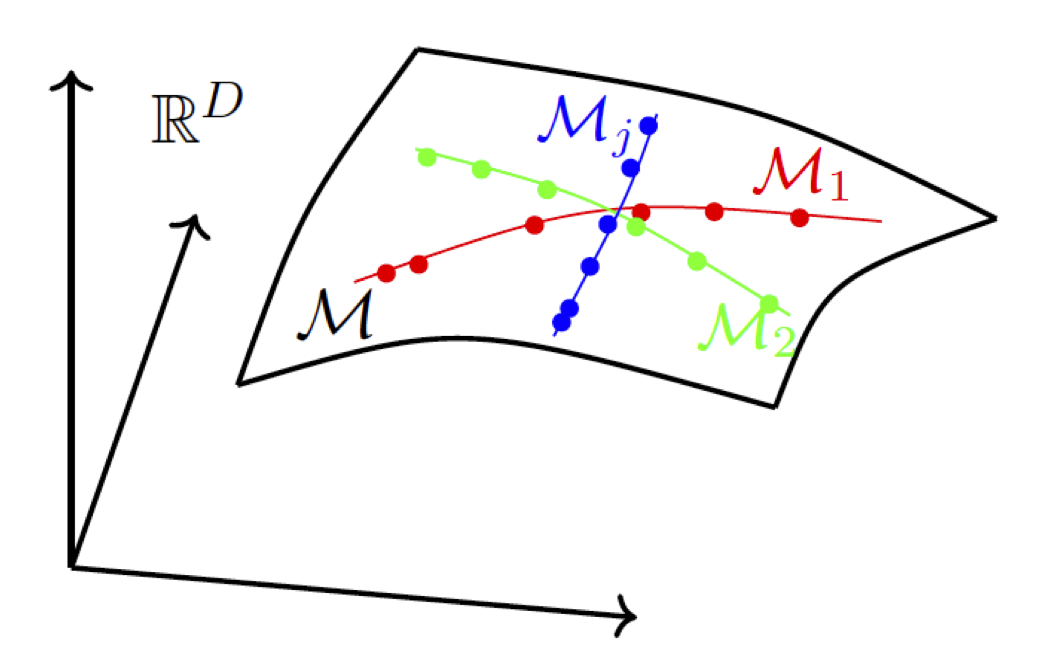
\includegraphics[width=0.5\linewidth]{\toplevelprefix/chapters/chapter3/figs/mixed-manifolds.png}
    \caption{Date distribuite pe un amestec de subvarietăți cu dimensiuni reduse $\cup_j \mathcal{M}_j$ într-un spațiu ambiental cu dimensiuni foarte mari, să zicem $\mathbb{R}^D$.}
    \label{fig:mixture-manifolds}
\end{figure}


\section{Minimizarea Entropiei și Compresie}

\subsection{Entropie și Rata de Codificare}
În \Cref{ch:intro}, am menționat că scopul învățării este de a găsi cel mai simplu mod de a genera un set dat de date. Conceptual, complexitatea Kolmogorov a fost destinată să ofere o astfel de măsură a complexității, dar nu este calculabilă și nu este asociată cu nicio schemă implementabilă care să poată reproduce efectiv datele. Prin urmare, avem nevoie de o măsură alternativă, calculabilă și realizabilă a complexității. Aceasta ne conduce la noțiunea de {\em entropie}, introdusă de Shannon în 1948 \cite{Shannon-1948}.

Pentru a ilustra natura constructivă a entropiei, să începem cu cel mai simplu caz. Să presupunem că avem o variabilă aleatoare discretă care ia $N$ valori distincte, sau \textit{jetoane}, $\{\x_1, \ldots, \x_N\}$ cu probabilitate egală $1/N$. Atunci am putea codifica fiecare jeton \(\vx_{i}\) folosind reprezentarea binară pe \(\log_2 N\)-biți a lui \(i\). Această schemă de codificare ar putea fi generalizată la codificarea distribuțiilor discrete arbitrare \cite{Cover-Thomas}: Dată o distribuție \(p\) astfel încât $\sum_{i=1}^N p(\x_i) = 1$, am putea atribui fiecărui jeton $\x_i$ cu probabilitate $p(\x_i)$ un cod binar de dimensiune $\log_2 [1/p(\x_i)] = - \log_2 p(\x_i)$ biți. Prin urmare, numărul mediu de biți, sau {\em rata de codificare}, necesară pentru a codifica orice eșantion din distribuția $p(\cdot)$ este dată de expresia:\footnote{Prin convenția Teoriei Informației \cite{Cover-Thomas}, $\log$ aici este în baza $2$. Prin urmare, entropia este măsurată în biți (binari).}
\begin{equation}
	H(\x) \doteq \mathbb{E}[\log 1/p(\x)]  = - \sum_{i=1}^N p(\x_i) \log  p(\x_i).
	\label{eqn:entropy-discrete}
\end{equation}
Aceasta este cunoscută ca {\em entropia} distribuției (discrete) $p(\cdot)$. Observați că această entropie este întotdeauna nenegativă și este zero dacă și numai dacă $p(\x_i) = 1$ pentru un anumit $\x_i$ cu $i \in [N]$.\footnote{Aici observăm că folosim faptul $\lim_{p\rightarrow 0} p \log p = 0$.}


\subsection{Entropie Diferențială}

Când variabila aleatoare $\x \in \R^{D}$ este continuă și are o densitate de probabilitate $p$, se poate considera că limita sumei de mai sus \eqref{eqn:entropy-discrete} este legată de o integrală:
\begin{equation}
	h(\vx) \doteq \Ex[\log 1/p(\vx)] = - \int_{\R^{D}} p(\vxi) \log p(\vxi) \odif{\vxi}.
	\label{eqn:entropy-differential}
\end{equation}
{Mai precis, dată o variabilă continuă $\x$, o putem cuantiza cu o dimensiune de cuantizare $\epsilon > 0$. Notând variabila discretă rezultată ca $\x^\epsilon$. Atunci se poate arăta că $H(\vx^\epsilon) + \log(\epsilon) \approx h(\vx)$. Prin urmare, când $\epsilon$ este mic, entropia diferențială $h(\x)$ poate fi negativă. Cititorii interesați pot consulta \cite{Cover-Thomas} pentru o explicație mai detaliată.}

\begin{example}[Entropia Distribuțiilor Gaussiene]
	Prin calcul direct, este posibil să arătăm că entropia unei distribuții Gaussiene $x \sim \mathcal{N}(\mu, \sigma^2)$ este dată de:
	\begin{equation}
		h(x) = \frac{1}{2}\log (2\pi \sigma^2) + \frac{1}{2}.
		\label{eqn:entropy-Gaussian}
	\end{equation}
	Se știe, de asemenea, că distribuția Gaussiană atinge entropia maximă
	pentru toate distribuțiile cu aceeași varianță $\sigma^2$. Entropia unei distribuții Gaussiene multivariate $\x \sim \mathcal{N}(\boldsymbol{\mu}, \boldsymbol{\Sigma})$ în $\mathbb{R}^D$ este dată de:
	\begin{equation}
		h(\x) = \frac{D}{2}(1 + \log(2\pi)) + \frac{1}{2}\log\det(\boldsymbol{\Sigma}).
		\label{eqn:entropy-Gaussian-multi}
	\end{equation}
\end{example}

Similar cu entropia pentru o distribuție discretă, am dori ca entropia
diferențială să fie asociată cu rata de codificare a unei scheme de codificare realizabile. De exemplu, ca mai sus, putem discretiza domeniul distribuției cu o grilă de dimensiune $\epsilon >0$. Rata de codificare a distribuției discrete rezultate poate fi văzută ca o aproximare a entropiei diferențiale \cite{Cover-Thomas}.

Fiți conștienți că există unele avertismente asociate cu definiția entropiei
diferențiale. Pentru o distribuție într-un spațiu cu dimensiuni mari, când suportul său devine degenerat (cu dimensiuni reduse), entropia sa diferențială diverge la \(-\infty\). Acest fapt este demonstrat în
\Cref{thm:max_entropy} (reamintim și caracterizarea entropiei maxime a distribuției Gaussiene menționată mai sus în \Cref{thm:max_entropy}) dar chiar și în cazul explicit simplu al distribuțiilor Gaussiene \eqref{eqn:entropy-Gaussian-multi}, când covarianța \(\vSigma\) este singulară, putem vedea că \(\log\det(\vSigma) = -\infty\) deci avem $h(\x) = -\infty$. Într-o astfel de situație, nu este evident cum să cuantizăm sau să codificăm în mod adecvat o astfel de distribuție. Cu toate acestea, distribuțiile degenerate (Gaussiene) sunt tocmai cele mai simple posibile, și fără îndoială cele mai importante, instanțe ale distribuțiilor cu dimensiuni reduse într-un spațiu cu dimensiuni mari. În acest capitol, vom discuta o rezolvare completă a acestei dificultăți aparente cu degenerarea.

\subsection{Minimizarea Ratei de Codificare}\label{sub:min_entropy}
Amintiți-vă că problema învățării implică recuperarea unei distribuții (potențial continue) $p(\x)$ dintr-un set de eșantioane $\{\x_1, \ldots, \x_N\}$ extrase din distribuție. Pentru ușurința expunerii, scriem $\X = [\x_1, \ldots, \x_N] \in \mathbb{R}^{D\times N}$. Având în vedere că distribuțiile de interes aici sunt (aproape) cu dimensiuni reduse, ar trebui să ne așteptăm ca entropia lor (diferențială) să fie foarte mică. Dar, spre deosebire de situațiile pe care le-am studiat în capitolul anterior, în general nu cunoaștem familia de modele (analitice) cu dimensiuni reduse căreia îi aparține distribuția $p(\x)$. Deci verificarea dacă entropia este mică pare să fie singura orientare pe care ne putem baza pentru a identifica și modela distribuția.

Acum, având doar eșantioanele fără a ști ce este $p(\x)$, în teorie ele ar putea fi interpretate ca eșantioane din orice distribuție generică. În special, ele ar putea fi interpretate ca oricare dintre următoarele cazuri:
\begin{enumerate}
	\item ca eșantioane din distribuția empirică $p^{\vX}$ însăși, care atribuie probabilitate $1/N$ fiecăruia dintre cele $N$ eșantioane $\x_i, i=1, \ldots, N$.
	\item ca eșantioane dintr-o distribuție normală standard $\x^n \sim p^{n} \doteq \mathcal{N}(\boldsymbol{0}, \sigma^2 \boldsymbol{I})$ cu o varianță $\sigma^2$ suficient de mare (să zicem mai mare decât normele eșantionului);
	\item ca eșantioane dintr-o distribuție normală $\x^e \sim p^{e} \doteq \mathcal{N}(\boldsymbol{0}, \hat{\vSigma})$ cu o covarianță $\hat{\vSigma} = \frac{1}{N} \X \X^T$ fiind covarianța empirică a eșantioanelor;
	\item ca eșantioane dintr-o distribuție $\hat \x \sim \hat{q}(\vx)$ care aproximează îndeaproape distribuția adevărată $p$.
\end{enumerate}
Acum întrebarea este: care este mai bună și în ce sens? Să presupunem că credeți că aceste date $\X$ sunt extrase dintr-o distribuție particulară $q(\x)$, care poate fi una dintre distribuțiile considerate mai sus. Atunci am putea codifica punctele de date cu cartea de coduri optimă pentru distribuția $q(\x)$. Lungimea medie de codificare necesară (sau rata de codificare) este dată de:
\begin{equation}
	\frac{1}{N}\sum_{i=1}^N -\log q(\x_i) \quad \approx \quad - \int_{\R^{D}} p(\vxi) \log q(\vxi)\odif{\vxi}
\end{equation}
pe măsură ce numărul de eșantioane $N$ devine mare. Dacă am identificat distribuția corectă $p(\x)$, rata de codificare este dată de entropia $- \int p(\vxi) \log p(\vxi) \odif{\vxi}$. Se dovedește că lungimea de codificare de mai sus $- \int p(\vxi) \log q(\vxi) \odif{\vxi}$ este întotdeauna mai mare sau egală cu entropia, cu excepția cazului în care $q(\x) = p(\x)$. Diferența lor, notată ca
\begin{eqnarray}
	\KL(p \mmid q) &\doteq& - \int_{\R^{D}} p(\vxi) \log q(\vxi) \odif{\vxi}  - \Big(- \int_{\R^{D}} p(\vxi) \log p(\vxi) \odif{\vxi} \Big)\\
	&=& \int_{\R^{D}} p(\vxi) \log \frac{p(\vxi)}{q(\vxi)} \odif{\vxi}
\end{eqnarray}
este cunoscută ca divergența {\em Kullback-Leibler} (KL), sau entropie relativă. Această cantitate este întotdeauna nenegativă.
\begin{theorem}[Inegalitatea Informației]\label{thm:information-inequality}
	Fie $p(\x), q(\x)$ două funcții de densitate de probabilitate (care au același
	suport). Atunci $\KL(p\mmid q) \ge 0$, unde inegalitatea devine egalitate dacă și numai dacă $p = q$.\footnote{Tehnic, această egalitate ar trebui să fie interpretată ca „aproape peste tot", i.e., cu excepția posibilă a unui set de măsură zero (volum), deoarece acest set nu ar afecta valoarea oricărei integrale.}
\end{theorem}
\begin{proof}
	\begin{eqnarray*}
		- \KL(p\mmid q)
		&=& - \int_{\R^{D}} p(\vxi) \log \frac{p(\vxi)}{q(\vxi)} \odif{\vxi}
		=  \int_{\R^{D}} p(\vxi) \log \frac{q(\vxi)}{p(\vxi)} \odif{\vxi} \\
		&\le& \log \int_{\R^{D}} p(\vxi)  \frac{q(\vxi)}{p(\vxi)} \odif{\vxi} \label{eqn:jensen-KL}
		= \log \int_{\R^{D}} q(\vxi) \odif{\vxi} = \log 1 = 0,
	\end{eqnarray*}
	unde prima inegalitate urmează din {\em inegalitatea lui Jensen} și
	faptul că funcția $\log(\cdot)$ este strict concavă. Egalitatea este valabilă
	dacă și numai dacă $p = q$ .
\end{proof}

Prin urmare, dat un set de date eșantionate $\X$, pentru a determina care caz este mai bun dintre $p^{n}$, $p^{e}$ și $\hat{q}$, putem compara ratele lor de codificare pentru $\X$ și putem vedea care oferă cea mai mică rată. Știm din cele de mai sus că rata de codificare (teoretic realizabilă) pentru o distribuție este strâns legată de entropia sa. În general, avem:
\begin{equation}
	h(\x^n) > h(\x^e) > h(\hat \x).
\end{equation}
Prin urmare, dacă datele $\X$ ar fi codificate de cartea de coduri asociată cu fiecare dintre aceste distribuții, rata de codificare pentru $\X$ ar scădea în general în aceeași ordine:
\begin{equation}
	p(\x^n) \rightarrow p(\x^e) \rightarrow p(\hat \x).
\end{equation}

Această observație ne oferă o orientare generală despre cum am putea fi capabili să urmărim o distribuție $p(\x)$ care are o structură cu dimensiuni reduse. Ea sugerează două abordări posibile:
\begin{enumerate}
	\item Pornind de la o distribuție generală (să zicem o distribuție normală) cu entropie mare, transformând treptat distribuția către distribuția (empirică) a datelor prin reducerea entropiei.
	\item Dintre o familie mare de distribuții (parametrice sau neparametrice) cu scheme de codificare explicite care codifică datele date, căutând progresiv scheme de codificare mai bune care dau rate de codificare mai mici.
\end{enumerate}
Conceptual, ambele abordări încearcă în esență să facă același lucru. Pentru prima abordare, trebuie să ne asigurăm că o astfel de cale de transformare există și este calculabilă. Pentru a doua abordare, este necesar ca familia aleasă să fie suficient de bogată și să poată aproxima îndeaproape (sau să conțină) distribuția adevărată. Pentru oricare dintre abordări, trebuie să ne asigurăm că soluțiile cu entropie mai mică sau rate de codificare mai bune pot fi calculate eficient și converg rapid către distribuția dorită.\footnote{Să zicem distribuția datelor din lumea reală, cum ar fi imagini și texte.} Vom explora ambele abordări în cele două secțiuni rămase ale acestui capitol.  %

\section{Compresie prin Îndepărtarea Zgomotului}\label{sub:compression_denoising}

În această secțiune, vom descrie o modalitate \textit{naturală} și \textit{tractabilă computațional} de a învăța o distribuție \(p(\vx)\) prin învățarea unei codificări parametrice a distribuției noastre astfel încât reprezentarea să aibă entropia sau rata de codificare minimă, apoi folosind această codificare pentru a transforma eșantioane cu entropie mare dintr-o distribuție Gaussiană standard în eșantioane cu entropie mică din distribuția țintă, așa cum este ilustrat în \Cref{fig:diffusion-chapter3}. Aceasta prezintă o metodologie care utilizează ambele abordări de mai sus pentru a învăța și eșantiona din distribuție.

\begin{figure}[t]
	\centering
	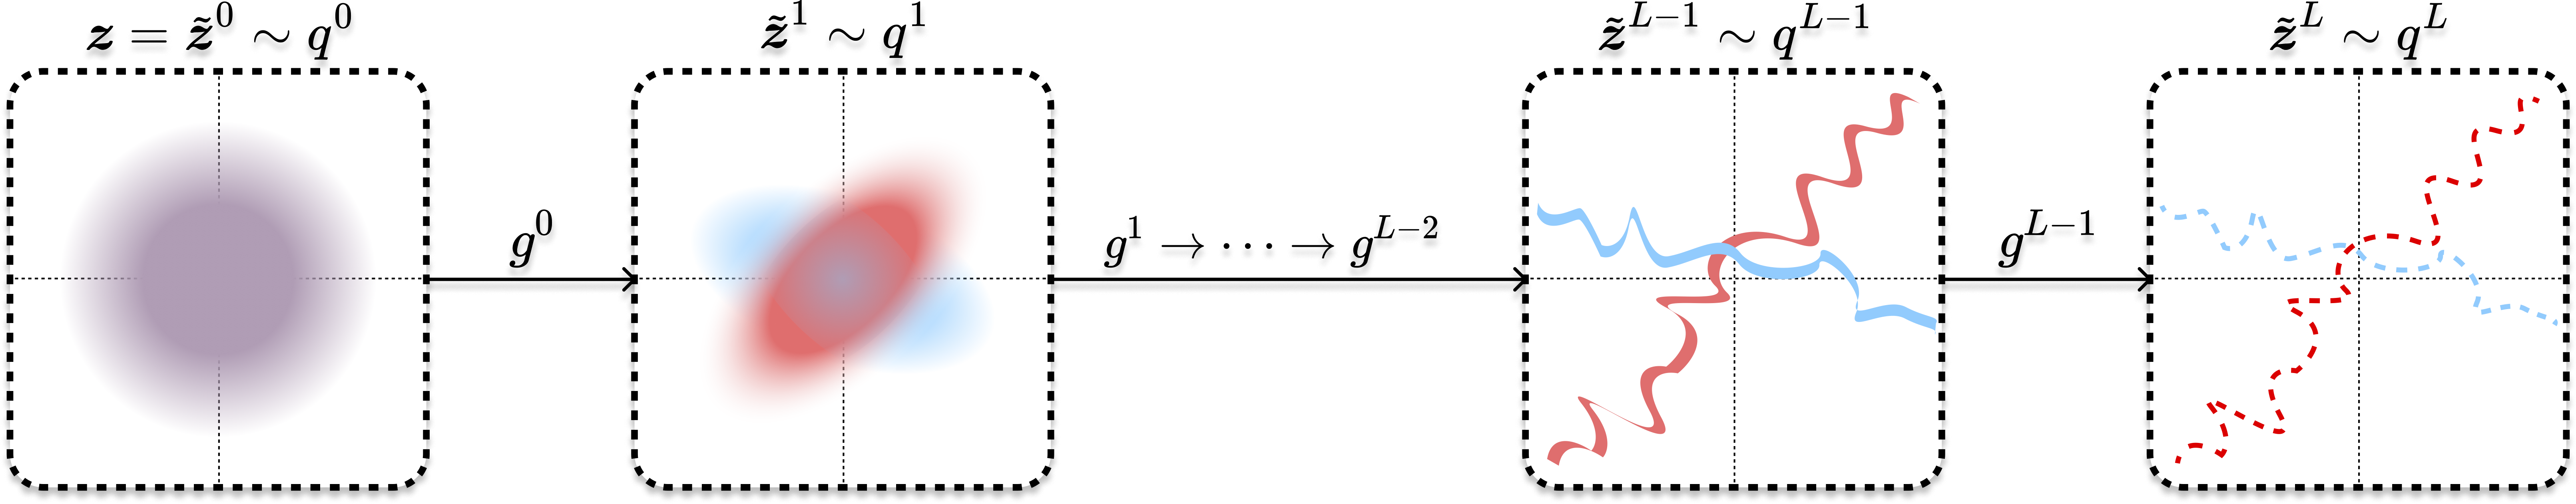
\includegraphics[width=\linewidth]{\toplevelprefix/chapters/chapter3/figs/diffusion_pipeline.png}
	\caption{Ilustrarea unui proces iterativ de îndepărtare a zgomotului care, pornind de la o distribuție Gaussiană izotropă, converge către o distribuție arbitrară de date.}
	\label{fig:diffusion-chapter3}
\end{figure}

\subsection{Procese de Difuzie și Îndepărtarea Zgomotului} \label{sub:intro_diffusion_denoising}

Mai întâi vrem să găsim o procedură pentru a scădea entropia unui eșantion foarte zgomotos dat într-un eșantion cu entropie mai mică din distribuția datelor. Aici, descriem o abordare potențială—una dintre multe, dar poate cel mai natural mod de a ataca această problemă. Mai întâi, găsim o modalitate de a \textit{crește treptat} entropia eșantioanelor existente din distribuția datelor. Apoi, găsim un \textit{invers aproximativ} al acestui proces. Dar în general, operația de creștere a entropiei nu are invers, deoarece informațiile din distribuția originală pot fi distruse. Vom aborda astfel un caz special în care (1) operația de adăugare a entropiei ia o formă simplă, calculabilă și reversibilă; (2) putem obține o codificare (parametrică) a distribuției datelor, așa cum am aluzionat în perechea de abordări de mai sus. După cum vom vedea, cei doi factori de mai sus vor asigura că abordarea noastră este posibilă.

Vom crește entropia în modul probabil cel mai simplu posibil, i.e., \textit{adăugând zgomot Gaussian izotrop}. Mai precis, dată variabila aleatoare \(\vx\), putem considera \textit{procesul stocastic} \((\vx_{t})_{t \in [0, T]}\) care adaugă zgomot treptat la aceasta, i.e.,
\begin{equation}\label{eq:additive_gaussian_noise_model}
	\vx_{t} \doteq \vx + t\vg, \qquad \forall t \in [0, T],
\end{equation}
unde \(T \in [0, \infty)\) este un orizont de timp și \(\vg \sim \dNorm(\vzero, \vI)\) este extras independent de \(\vx\). Acest proces este un exemplu de \textit{proces de difuzie}, numit astfel deoarece împrăștie masa de probabilitate pe tot \(\R^{D}\) pe măsură ce timpul trece, crescând entropia în timp. Această intuiție este confirmată grafic de \Cref{fig:ve_forward_density} și riguros prin următoarea teoremă.
\begin{theorem}[Versiune Simplificată a \Cref{thm:diffusion_entropy_increases}]
	Să presupunem că \((\vx_{t})_{t \in [0, T]}\) urmează modelul \eqref{eq:additive_gaussian_noise_model}. Pentru orice \(t \in (0, T]\), variabila aleatoare \(\vx_{t}\) are entropie diferențială \(h(\vx_{t}) > -\infty\). Mai mult, în anumite condiții tehnice pe \(\vx\), 
	\begin{equation}
		\odv*{h(\vx_{t})}{t} > 0, \qquad \forall t \in (0, T],
	\end{equation}
	arătând că entropia lui \(\vx\) cu zgomot crește în timp \(t\).
\end{theorem}
Demonstrația este elementară, dar este destul de lungă, așa că o amânăm pentru \Cref{sub:diffusion_entropy_increases}. Principala implicație încă nenunțată a acestui rezultat este că \(h(\vx_{t}) > h(\vx)\) pentru fiecare \(t > 0\). Pentru a vedea aceasta, observați că dacă \(h(\vx) = -\infty\) atunci \(h(\vx_{t}) > -\infty\) pentru toți \(t > 0\), și dacă \(h(\vx) > -\infty\) atunci \(h(\vx_{t}) = h(\vx) + \int_{0}^{t}[\odv*{h(\vx_{s})}{s}]\odif{s} > h(\vx)\) prin teorema fundamentală a calculului, deci în ambele cazuri \(h(\vx_{t}) > h(\vx)\) pentru fiecare \(t > 0\).

\begin{figure}
	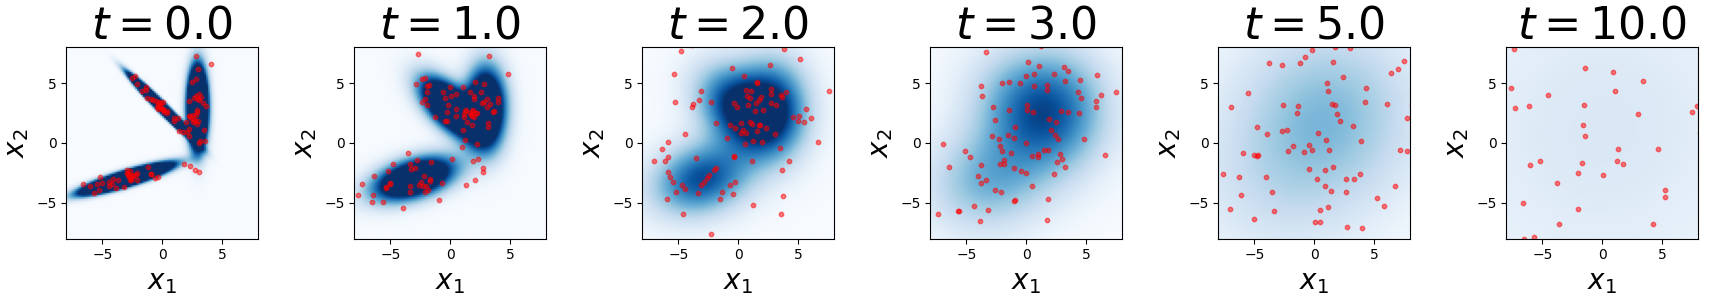
\includegraphics[width=\textwidth]{\toplevelprefix/chapters/chapter3/figs/ve_forward_diffusion_density.png}
	\caption{\small\textbf{Difuzarea unui amestec de Gaussiene.} De la stânga la dreapta, observăm evoluția densității pe măsură ce \(t\) crește de la \(0\) la \(10\), împreună cu câteva eșantioane reprezentative. Fiecare regiune este colorată în funcție de densitatea sa (\(0.0\) este complet alb, \(> 0.01\) este albastru foarte închis, orice altă valoare se mapează la o nuanță de albastru între acestea.) Observăm că masa de probabilitate devine mai puțin concentrată pe măsură ce \(t\) crește, semnalând că entropia crește.}
	\label{fig:ve_forward_density}
\end{figure}

Operația inversă adăugării de zgomot este cunoscută ca \textit{îndepărtarea zgomotului}. Este un subiect clasic și bine studiat în procesarea semnalului și teoria sistemelor, cum ar fi filtrul Wiener și filtrul Kalman. Câteva probleme discutate în \Cref{ch:classic}, cum ar fi PCA, ICA și Învățarea Dicționarului, sunt instanțe specifice ale problemei de îndepărtare a zgomotului. Pentru un \(t\) fix și modelul de zgomot Gaussian aditiv \eqref{eq:additive_gaussian_noise_model}, problema de îndepărtare a zgomotului poate fi formulată ca încercarea de a învăța o funcție \(\bar{\vx}^{\ast}(t, \cdot)\) care formează cea mai bună aproximare posibilă (în așteptare) a variabilei aleatoare adevărate \(\vx\), date fiind atât \(t\) cât și \(\vx_{t}\):
\begin{equation}\label{eq:denoising_loss}
	\bar{\vx}^{\ast}(t, \cdot) \in \argmin_{\bar{\vx}(t, \cdot)}\Ex_{\vx, \vx_{t}}\norm{\vx - \bar{\vx}(t, \vx_{t})}_{2}^{2}.
\end{equation}
Soluția acestei probleme, când optimizăm \(\bar{\vx}(t, \cdot)\) peste toate funcțiile posibile (integrabile pătratic), este așa-numitul \textit{denoiser optim Bayes}: 
\begin{equation}\label{eq:optimal_denoiser}
	\bar{\vx}^{\ast}(t, \vxi) \doteq \Ex[\vx \mid \vx_{t} = \vxi].
\end{equation}

Această expresie justifică notația \(\bar{\vx}\), care este menită să calculeze o așteptare condiționată (i.e., medie condiționată sau medie condiționată). Pe scurt, încearcă să elimine zgomotul din intrarea zgomotoasă, producând cea mai bună estimare posibilă (în așteptare și în raport cu distanța \(\ell^{2}\)) a variabilei aleatoare originale (fără zgomot).

\begin{example}[Îndepărtarea Zgomotului Gaussian dintr-un Amestec de Gaussiene]\label{example:denoising_gaussian_mixture}
	În acest exemplu calculăm denoiser-ul optim Bayes pentru o clasă incredibil de importantă de distribuții, modelul de amestec Gaussian. Pentru a începe, să fixăm parametrii pentru distribuție: ponderile amestecului \(\vpi \in \R^{K}\), mediile componentelor \(\{\vmu_{k}\}_{k = 1}^{K} \subseteq \R^{D}\), și covarianțele componentelor \(\{\vSigma_{k}\}_{k = 1}^{K} \subseteq \PSD(D)\), unde \(\PSD(D)\) este mulțimea matricelor simetrice pozitiv semidefinite de \(D \times D\). Acum, să presupunem că \(\vx\) este generat prin următoarea procedură în doi pași:
	\begin{itemize}
		\item Mai întâi, un index (sau \textit{etichetă}) \(y \in [K]\) este eșantionat astfel încât \(y = k\) cu probabilitate \(\pi_{k}\).
		\item În al doilea rând, \(\vx\) este eșantionat din distribuția normală \(\dNorm(\vmu_{y}, \vSigma_{y})\).
	\end{itemize}
	Atunci \(\vx\) are distribuția
	\begin{equation}
		\vx \sim \sum_{k = 1}^{K}\pi_{k}\dNorm(\vmu_{k}, \vSigma_{k}),
	\end{equation}
	și astfel
	\begin{equation}
		\vx_{t} = \vx + t\vg \sim \sum_{k = 1}^{K}\pi_{k}\dNorm(\vmu_{k}, \vSigma_{k} + t^{2}\vI).
	\end{equation}
	Să definim \(\phi(\vx ; \vmu, \vSigma)\) ca densitatea de probabilitate a \(\dNorm(\vmu, \vSigma)\) evaluată la \(\vx\). În această notație, densitatea lui \(\vx_{t}\) este
	\begin{equation}
		p_{t}(\vx_{t}) = \sum_{k = 1}^{K}\pi_{k}\phi(\vx_{t} ; \vmu_{k}, \vSigma_{k} + t^{2}\vI).
	\end{equation}

	Condiționat pe \(y\), variabilele sunt în comun Gaussiene: dacă spunem că \(\vx = \vmu_{y} + \vSigma_{y}^{1/2}\vu\) unde \((\cdot)^{1/2}\) este rădăcina pătrată a matricei și \(\vu \sim \dNorm(\vzero, \vI)\) independent de \(y\) (și \(\vg\)), atunci avem
	\begin{equation}
		\mat{\vx \\ \vx_{t}} = \mat{\vmu_{y} \\ \vmu_{y}} + \mat{\vSigma_{y}^{1/2} & \vzero \\ \vSigma_{y}^{1/2} & t\vI}\mat{\vu \\ \vg}.
	\end{equation}
	Aceasta arată că \(\vx\) și \(\vx_{t}\) sunt în comun Gaussiene (condiționate pe \(y\)) așa cum am afirmat. Astfel putem scrie
	\begin{equation}
		\mat{\vx \\ \vx_{t}} \sim \dNorm\rp{\mat{\vmu_{y} \\ \vmu_{y}}, \mat{\vSigma_{y} & \vSigma_{y} \\ \vSigma_{y} & \vSigma_{y} + t^{2}\vI}}.
	\end{equation}
	Astfel așteptarea condiționată a lui \(\vx\) dată \(\vx_{t}\) (i.e., denoiser-ul
	optim Bayes condiționat pe \(y\)) este faimos
	(\Cref{exercise:conditional_gaussian})
	\begin{equation}
		\Ex[\vx \mid \vx_{t}, y] = \vmu_{y} + \vSigma_{y}(\vSigma_{y} + t^{2}\vI)^{-1}(\vx_{t} - \vmu_{y}).
	\end{equation}
	Pentru a găsi denoiser-ul optim Bayes general, folosim legea așteptării iterate, obținând
	\begin{align}
		\bar{\vx}^{\ast}(t, \vx_{t})
		&= \Ex[\vx \mid \vx_{t}] \\ 
		&= \Ex[\Ex[\vx \mid \vx_{t}, y] \mid \vx_{t}] \\ 
		&= \sum_{k = 1}^{K}\Pr[y = k \mid \vx_{t}]\Ex[\vx \mid \vx_{t}, y = k].
	\end{align}
	Probabilitatea poate fi tratată după cum urmează. Fie \(p_{t \mid y}\) densitatea de probabilitate a lui \(\vx_{t}\) condiționată pe valoarea lui \(y\). Atunci
	\begin{align}
		\Pr[y = k \mid \vx_{t}]
		&= \frac{p_{t \mid y}(\vx_{t} \mid k)\pi_{k}}{p_{t}(\vx_{t})} \\ 
		&= \frac{\pi_{k}\phi(\vx_{t} ; \vmu_{k}, \vSigma_{k}
		+ t^{2}\vI)}{\sum_{i = 1}^{K}\pi_{i}\phi(\vx_{t} ; \vmu_{i}, \vSigma_{i} + t^{2}\vI)}.
	\end{align}
	Pe de altă parte, așteptarea condiționată este așa cum am descris înainte:
	\begin{equation}
		\Ex[\vx \mid \vx_{t}, y = k] = \vmu_{k} + \vSigma_{k}(\vSigma_{k} + t^{2}\vI)^{-1}(\vx_{t} - \vmu_{k}).
	\end{equation}
	Deci punând toate acestea împreună, adevăratul denoiser optim Bayes este
	\begin{equation}\label{eq:gmm_bayes_optimal_denoiser}
		\bar{\vx}^{\ast}(t, \vx_{t}) = \sum_{k = 1}^{K}\frac{\pi_{k}\phi(\vx_{t}
		;\vmu_{k}, \vSigma_{k} + t^{2}\vI)}{\sum_{i = 1}^{K}\pi_{i}\phi(\vx_{t}
		;\vmu_{i}, \vSigma_{i} + t^{2}\vI)}\cdot\bp{\vmu_{k} + \vSigma_{k}(\vSigma_{k} + t^{2}\vI)^{-1}(\vx_{t} - \vmu_{k})}.
	\end{equation}
	Acest exemplu este deosebit de important, și câteva cazuri speciale ne vor oferi o mare intuiție conceptuală mai târziu. Pentru moment, să încercăm să extragem o anumită intuiție geometrică din forma funcțională a denoiser-ului optim \eqref{eq:gmm_bayes_optimal_denoiser}.

	Pentru a încerca să înțelegem \eqref{eq:gmm_bayes_optimal_denoiser} intuitiv, să setăm mai întâi \(K = 1\) (i.e., o Gaussiană) astfel încât \(\vx \sim \dNorm(\vmu, \vSigma)\). Să diagonalizăm apoi \(\vSigma = \vV\vLambda \vV^{\top}\). Atunci denoiser-ul optim Bayes este
	\begin{equation}
		\bar{\vx}^{\ast}(t, \vx_{t}) = \vmu + \vSigma(\vSigma + t^{2}\vI)^{-1}(\vx_{t} - \vmu) = \vmu + \vV\mat{\lambda_{1}/(\lambda_{1} + t^{2}) & & \\ & \ddots & \\ & & \lambda_{D}/(\lambda_{D} + t^{2})}\vV^{\top}(\vx_{t} - \vmu),
	\end{equation}
	unde \(\lambda_{1}, \dots, \lambda_{D}\) sunt valorile proprii ale lui \(\vSigma\). Putem observa că acest denoiser are trei pași:
	\begin{itemize}
		\item Translatează intrarea \(\vx_{t}\) cu \(\vmu\).
		\item Contractă intrarea (translată) \(\vx_{t} - \vmu\) în fiecare direcție a vectorului propriu cu o cantitate \(\lambda_{i}/(\lambda_{i} + t^{2})\). Dacă intrarea translată este de rang redus și unele valori proprii ale lui \(\vSigma\) sunt zero, aceste direcții sunt imediat contractate la \(0\) de către denoiser, asigurând că ieșirea contracției este similar de rang redus.
		\item Translatează ieșirea înapoi cu \(\vmu\).
	\end{itemize}
	Este ușor de arătat că contractă actualul \(\vx_{t}\) către media \(\vmu\):
	\begin{equation}\label{eq:contraction}
		\norm{\bar{\vx}^{\ast}(t, \vx_{t}) - \vmu}_{2} \leq \norm{\vx_{t} - \vmu}_{2}.
	\end{equation}

	Aceasta este interpretarea geometrică a denoiser-ului unei \textit{singure} Gaussiene. Denoiser-ul general al modelului de amestec Gaussian \eqref{eq:gmm_bayes_optimal_denoiser} folosește \(K\) astfel de denoisere, ponderând ieșirea lor cu probabilitățile posterioare \(\Pr[y = k \mid \vx_{t}]\). Dacă mediile Gaussienelor sunt bine separate, aceste probabilități posterioare sunt foarte aproape de \(0\) sau \(1\) în apropierea fiecărei medii sau cluster. În acest regim, denoiser-ul general \eqref{eq:gmm_bayes_optimal_denoiser} are aceeași interpretare geometrică ca denoiser-ul cu o singură Gaussiană de mai sus.

	La prima vedere, o astfel de mapare de contracție \eqref{eq:contraction} poate părea similară cu iterațiile puterii (vezi \Cref{subsec:power iterations}). Cu toate acestea, cele două sunt fundamental diferite. Iterația puterii implementează o mapare de contracție către un subspațiu---și anume subspațiul întins de prima componentă principală. În contrast, iterațiile din \eqref{eq:contraction} converg către media \(\vmu\) a distribuției subiacente, care este un singur punct.
\end{example}

\begin{figure}
	\centering 
	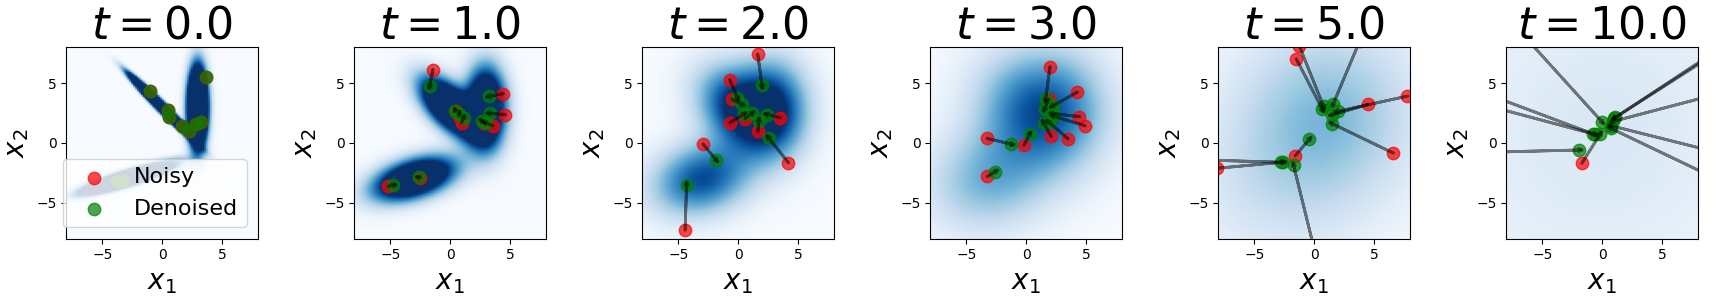
\includegraphics[width=\textwidth]{\toplevelprefix/chapters/chapter3/figs/ve_forward_diffusion_denoising.png}\vspace{-0.15in}
	\caption{\small \textbf{Denoiser-ul optim Bayes și scorul unui model de amestec Gaussian.} În aceeași setare ca \Cref{fig:ve_forward_density}, demonstrăm efectul denoiser-ului optim Bayes \(\bar{\vx}^{\ast}\) prin trasarea \(\vx_{t}\) (roșu) și \(\bar{\vx}^{\ast}(t, \vx_{t})\) (verde) pentru o anumită alegere \(t\) și \(\vx_{t}\). Prin formula lui Tweedie \Cref{thm:tweedie}, reziduul dintre ele este proporțional cu așa-numitul scor (Hyv\"arinen) \(\nabla_{\vx_{t}}\log p_{t}(\vx_{t})\). Putem vedea că scorul indică către modurile distribuției lui \(\vx_{t}\).}
	\label{fig:ve_forward_denoising}
\end{figure}

Intuitiv, și așa cum putem vedea din \Cref{example:denoising_gaussian_mixture}, denoiser-ul optim Bayes \(\bar{\vx}^{\ast}(t, \cdot)\) ar trebui să-și mute intrarea \(\vx_{t}\) către modurile distribuției lui \(\vx\). Se dovedește că, de fapt, putem cuantifica aceasta arătând că denoiser-ul optim Bayes \textit{face un pas de urcare a gradientului} pe densitatea (log-)densității lui \(\vx_{t}\), pe care (reamintim) am notat-o \(p_{t}\). Adică, urmând denoiser-ul înseamnă a te deplasa de la iterația de intrare într-o regiune cu probabilitate mai mare în cadrul acestei distribuții (perturbate). Pentru \(t\) mic, perturbarea este mică, deci intuiția noastră inițială este (aproape) exact corectă. Imaginea este vizualizată în \Cref{fig:ve_forward_denoising} și formulată riguros ca formula lui Tweedie \cite{Robbins1956AnEB}.
\begin{theorem}[Formula lui Tweedie]\label{thm:tweedie}
	Să presupunem că \((\vx_{t})_{t \in [0, T]}\) respectă \eqref{eq:additive_gaussian_noise_model}. Fie \(p_{t}\) densitatea lui \(\vx_{t}\) (așa cum a fost declarată anterior). Atunci
	\begin{equation}\label{eq:tweedie}
		\Ex[\vx \mid \vx_{t}] = \vx_{t} + t^{2}\nabla_{\vx_{t}} \log p_{t}(\vx_{t}).
	\end{equation}
\end{theorem}
\begin{proof}
	Pentru demonstrație să presupunem că \(\vx\) are o densitate (deși teorema
	este adevărată fără această presupunere), și să numim această densitate \(p\). Fie
	\(p_{0 \mid t}\) și \(p_{t \mid 0}\) densitățile condiționate ale lui \(\vx
	= \vx_{0}\) date \(\vx_{t}\) și \(\vx_{t}\) date \(\vx\) respectiv.
	Fie \(\phi(\vx ; \vmu, \vSigma)\) densitatea lui \(\dNorm(\vmu,
	\vSigma)\) evaluată la \(\vx\), astfel încât \(p_{t \mid 0}(\vx_{t} \mid \vx)
	= \phi(\vx_{t} ; \vx, t^{2}\vI)\). Atunci un calcul simplu dă
	\begin{align}
		\nabla_{\vx_{t}} \log p_{t}(\vx_{t})
		&= \frac{\nabla_{\vx_{t}}p_{t}(\vx_{t})}{p_{t}(\vx_{t})} \\
		&= \frac{1}{p_{t}(\vx_{t})}\nabla_{\vx_{t}}\int_{\R^{D}}p(\vx)p_{t \mid 0}(\vx_{t} \mid \vx)\odif{\vx} \\
		&=
		\frac{1}{p_{t}(\vx_{t})}\nabla_{\vx_{t}}\int_{\R^{D}}p(\vx)\phi(\vx_{t}
		;\vx, t^{2}\vI)\odif{\vx} \\
		&=
		\frac{1}{p_{t}(\vx_{t})}\int_{\R^{D}}p(\vx)[\nabla_{\vx_{t}}\phi(\vx_{t}
		;\vx, t^{2}\vI)]\odif{\vx} \\
		&= \frac{1}{p_{t}(\vx_{t})}\int_{\R^{D}}p(\vx)\phi(\vx_{t} ; \vx, t^{2}\vI)\bs{-\frac{\vx_{t} - \vx}{t^{2}}}\odif{\vx} \\
		&= \frac{1}{t^{2}p_{t}(\vx_{t})}\int_{\R^{D}}p(\vx)\phi(\vx_{t} ; \vx, t^{2}\vI)[\vx - \vx_{t}]\odif{\vx} \\
		&= \frac{1}{t^{2}p_{t}(\vx_{t})}\int_{\R^{D}}p(\vx)\phi(\vx_{t} ; \vx,
		t^{2}\vI)\vx \odif{\vx}
		- \frac{\vx_{t}}{t^{2}p_{t}(\vx_{t})}\int_{\R^{D}}p(\vx)\phi(\vx_{t} ; \vx, t^{2}\vI)\odif{\vx} \\
		&= \frac{1}{t^{2}p_{t}(\vx_{t})}\int_{\R^{D}}p(\vx)p_{t \mid 0}(\vx_{t} \mid \vx)\vx \odif{\vx} - \frac{\vx_{t}}{t^{2}p_{t}(\vx_{t})}p_{t}(\vx_{t}) \\
		&= \frac{1}{t^{2}p_{t}(\vx_{t})}\int_{\R^{D}}p_{t}(\vx_{t})p_{0 \mid t}(\vx \mid \vx_{t})\vx \odif{\vx} - \frac{\vx_{t}}{t^{2}p_{t}(\vx_{t})}p_{t}(\vx_{t}) \\
		&= \frac{1}{t^{2}}\int_{\R^{D}}p_{0 \mid t}(\vx \mid \vx_{t})\vx \odif{\vx} - \frac{\vx_{t}}{t^{2}} \\
		&= \frac{1}{t^{2}}\Ex[\vx \mid \vx_{t}] - \frac{\vx_{t}}{t^{2}} \\
		&= \frac{\Ex[\vx \mid \vx_{t}] - \vx_{t}}{t^{2}}.
	\end{align}
	Rearanjarea simplă a egalității de mai sus demonstrează teorema.
\end{proof}
Acest rezultat dezvoltă o conexiune între îndepărtarea zgomotului și optimizare: denoiser-ul optim Bayes face un singur pas de urcare a gradientului pe densitatea datelor perturbate \(p_{t}\), iar dimensiunea pasului devine adaptiv mai mică (i.e., făcând pași mai preciși) pe măsură ce perturbarea distribuției datelor devine mai mică. Cantitatea \(\nabla_{\vx_{t}}\log p_{t}(\vx_{t})\) este numită \textit{scorul (Hyv\"arinen)} și apare frecvent în discuții despre îndepărtarea zgomotului etc.; a apărut pentru prima dată într-o lucrare a lui Aapo Hyv\"arinen în contextul ICA \cite{hyvarinen05a}.

Similar cu modul în care un pas de coborâre a gradientului nu este aproape niciodată suficient pentru a minimiza un obiectiv în practică atunci când se inițializează departe de optim, ieșirea denoiser-ului optim Bayes \(\bar{\vx}^{\ast}(t, \cdot)\) nu este aproape niciodată conținută într-o regiune cu probabilitate mare a distribuției datelor când \(t\) este mare, \textit{în special} când datele au structuri cu dimensiuni reduse. Ilustrăm acest punct explicit în următorul exemplu.
\begin{example}[Îndepărtarea zgomotului dintr-un Amestec cu Două Puncte]\label{example:denoising_twopoints}
	Fie \(x\) uniformă pe mulțimea cu două puncte \(\{-1, +1\}\) și fie \((\vx_{t})_{t \in [0, T]}\) să urmeze \eqref{eq:additive_gaussian_noise_model}. Aceasta este tocmai un model de amestec Gaussian degenerat cu prioruri egale cu \(\frac{1}{2}\), medii \(\{-1, +1\}\) și covarianțe ambele egale cu \(0\). Pentru un \(t > 0\) fix putem folosi calculul denoiser-ului optim Bayes din \eqref{eq:gmm_bayes_optimal_denoiser} pentru a obține (demonstrație ca exercițiu)
	\begin{equation}
		\bar{x}^{\ast}(t, x_{t}) = \frac{\phi(x_{t} ; +1, t^{2}) - \phi(x_{t}
		; -1, t^{2})}{\phi(x_{t} ; 1, t^{2}) + \phi(x_{t} ; -1, t^{2})} = \tanh\rp{-\frac{x_{t}}{t^{2}}}.
	\end{equation}
	Pentru \(t\) aproape de \(0\), această cantitate este aproape de \(\{-1, +1\}\) pentru aproape toate intrările \(\bar{x}^{\ast}(t, x_{t})\). Cu toate acestea, pentru \(t\) mare, această cantitate nu este neapărat nici măcar aproximativ în suportul original al lui \(x\), care, amintim, este \(\{-1, +1\}\). În special, pentru \(x_{t} \approx 0\) avem \(\bar{x}^{\ast}(t, x_{t}) \approx 0\) care se află complet între cele două puncte posibile. Astfel \(\bar{x}^{\ast}\) \textit{nu va produce ``realist'' \(x\)}. Sau mai matematic, distribuția lui \(\bar{x}(t, x_{t})\) este foarte diferită de distribuția lui \(x\).
\end{example}

Prin urmare, dacă vrem să îndepărtăm zgomotul din eșantionul foarte zgomotos \(\vx_{T}\) (unde—reamintim—\(T\) este timpul maxim), nu putem folosi doar denoiser-ul \textit{o dată}. În schimb, trebuie să folosim denoiser-ul de multe ori, analog cu coborârea gradientului cu \textit{dimensiuni descrescătoare ale pasului}, pentru a converge la un punct staționar \(\hat{\vx}\). Și anume, vom folosi denoiser-ul pentru a merge de la \(\vx_{T}\) la \(\hat{\vx}_{T - \delta}\) care aproximează \(\vx_{T - \delta}\), apoi de la \(\hat{\vx}_{T - \delta}\) la \(\hat{\vx}_{T - 2\delta}\), etc., până de la \(\hat{\vx}_{\delta}\) la \(\hat{\vx} = \hat{\vx}_{0}\). De fiecare dată când facem un pas de îndepărtare a zgomotului, acțiunea denoiser-ului devine mai mult ca un pas de gradient pe (log-)densitatea originală.

Mai formal, discretizăm uniform \([0, T]\) în \(L + 1\) pași de timp \(0 = t_{0} < t_{1} < \cdots < t_{L} = T\), i.e.,
\begin{equation}
	t_{\ell} = \frac{\ell}{L}T, \qquad \ell \in \{0, 1, \dots, L\}.
\end{equation}
Apoi pentru fiecare \(\ell \in [L] = \{1, 2, \dots, L\}\), mergând de la \(\ell = L\) la \(\ell = 1\), putem rula iterația
\begin{align}
	\hat{\vx}_{t_{\ell - 1}}
	&= \Ex[\vx_{t_{\ell - 1}} \mid \vx_{t_{\ell}} = \hat{\vx}_{t_{\ell}}] \\
	&= \Ex[\vx + t_{\ell - 1}\vg \mid \vx_{t_{\ell}} = \hat{\vx}_{t_{\ell}}] \\
	&= \Ex\rs{\vx + t_{\ell - 1}\cdot\frac{\vx_{t_{\ell}} - \vx}{t_{\ell}} \given \vx_{t_{\ell}} = \hat{\vx}_{t_{\ell}}} \\
	&= \frac{t_{\ell - 1}}{t_{\ell}}\hat{\vx}_{t_{\ell}} + \bp{1 - \frac{t_{\ell - 1}}{t_{\ell}}}\Ex[\vx \mid \vx_{t_{\ell}} = \hat{\vx}_{t_{\ell}}] \\
	&= \bp{1 - \frac{1}{\ell}}\cdot\hat{\vx}_{t_{\ell}} + \frac{1}{\ell}\cdot\bar{\vx}^{\ast}(t_{\ell}, \hat{\vx}_{t_{\ell}}).
\end{align}
Efectul acestei iterații este următorul. La începutul iterației, unde \(\ell\) este mare, abia avem încredere în ieșirea denoiser-ului și păstrăm în mare parte iterația curentă. Aceasta are sens, deoarece denoiser-ul poate avea varianță uriașă (cf \Cref{example:denoising_twopoints}). Când \(\ell\) este mic, denoiser-ul va ``se fixa'' pe modurile distribuției datelor, deoarece un pas de îndepărtare a zgomotului face practic un pas de gradient pe log-densitatea distribuției adevărate, și putem avea încredere că nu va produce eșantioane nerezonabile, astfel încât pasul de îndepărtare a zgomotului implică în mare parte ieșirea denoiser-ului. La \(\ell = 1\) chiar aruncăm iterația curentă și păstrăm doar ieșirea denoiser-ului.

\begin{figure}[t]
	\centering
	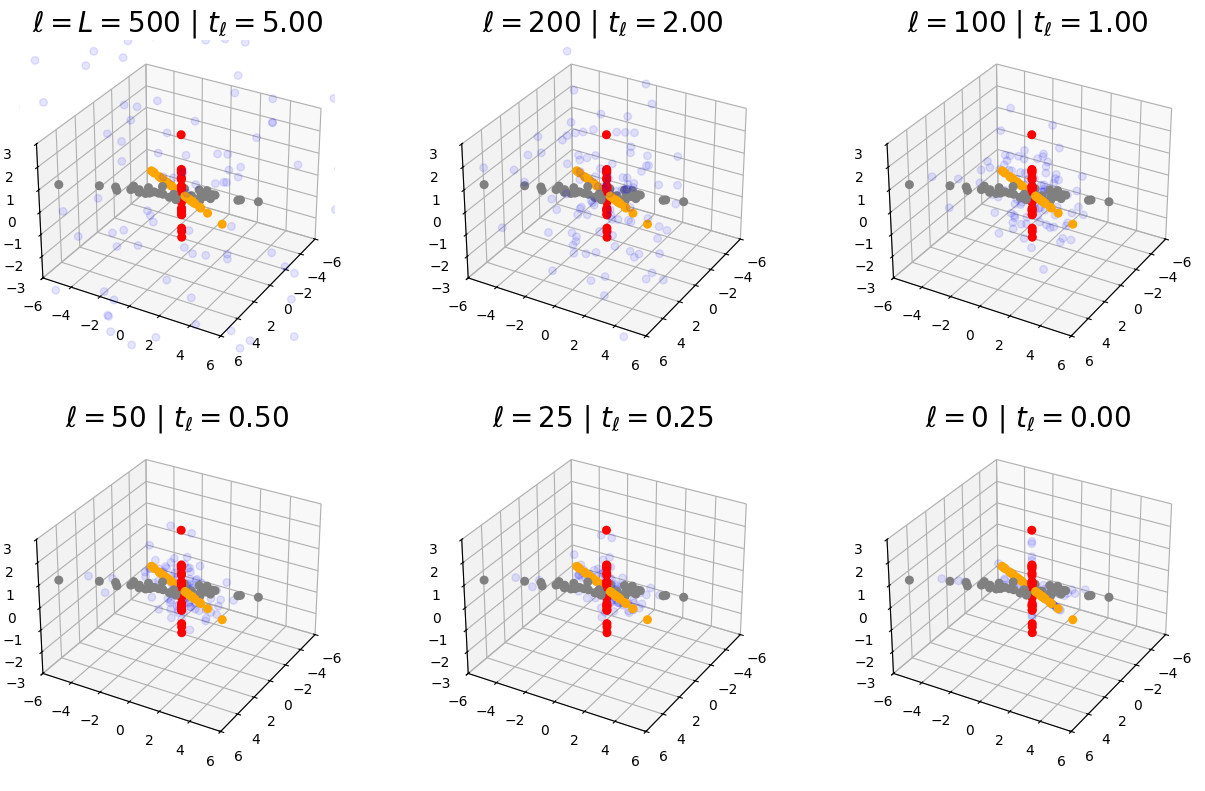
\includegraphics[width=\textwidth]{\toplevelprefix/chapters/chapter3/figs/ve_gmm_denoising.png}
	\caption{\small\textbf{Îndepărtarea zgomotului dintr-un amestec de Gaussiene de rang redus.} Fiecare figură reprezintă eșantioane din distribuția adevărată a datelor (gri, portocaliu, roșu) și eșantioane care trec prin procesul de îndepărtare a zgomotului \eqref{eq:denoising-iteration-basic} (albastru deschis). În stânga sus, procesul tocmai a început și zgomotul este foarte mare. Pe măsură ce procesul continuă, zgomotul este împins mai departe către suportul distribuției datelor de rang redus. În final, în dreapta jos, eșantioanele generate sunt perfect aliniate cu suportul datelor și arată foarte mult ca eșantioane extrase din modelul de amestec Gaussian de rang redus.}
	\label{fig:ve_gmm_denoising}
\end{figure}

Cele de mai sus sunt intuiția pentru care ne așteptăm ca procesul de îndepărtare a zgomotului să convergă. Vizualizăm procesul de convergență în \(\R^{3}\) în \Cref{fig:ve_gmm_denoising}. Vom dezvolta mai târziu câteva rezultate riguroase despre convergență. Pentru moment, amintiți-vă că am vrut să construim un proces pentru a reduce entropia. Deși am făcut acest lucru într-un mod indirect inversând un proces care adaugă entropie, acum este timpul să confirmăm că procesul nostru iterativ de îndepărtare a zgomotului reduce entropia.

\begin{theorem}[Versiune Simplificată a \Cref{thm:conditioning_reduces_entropy}]
	Să presupunem că \((\vx_{t})_{t \in [0, T]}\) respectă \eqref{eq:additive_gaussian_noise_model}. Atunci, în anumite condiții tehnice pe \(\vx\), pentru fiecare \(s < t\) cu \(s, t \in (0, T]\),
	\begin{equation}
		h(\Ex[\vx_{s} \mid \vx_{t}]) < h(\vx_{t}).
	\end{equation}
\end{theorem}
Enunțul complet al teoremei și demonstrația în sine necesită unele tehnicități, așa că este amânată pentru \Cref{sub:denoising_entropy_decreases}.

Ultimul lucru pe care îl discutăm aici este că de multe ori \textit{nu vom putea calcula} \(\bar{\vx}^{\ast}(t, \cdot)\) pentru niciun \(t\), deoarece nu avem distribuția \(p_{t}\). Dar putem încerca să \textit{învățăm una din date}. Amintiți-vă că denoiser-ul \(\bar{\vx}^{\ast}\) este definit în \eqref{eq:denoising_loss} ca minimizând eroarea pătratică medie \(\Ex\norm{\bar{\vx}(t, \vx_{t}) - \vx}_{2}^{2}\). Putem folosi această eroare pătratică medie ca o pierdere sau funcție obiectiv pentru a învăța denoiser-ul. De exemplu, putem parametriza \(\bar{\vx}(t, \cdot)\) printr-o rețea neurală, scriind-o ca \(\bar{\vx}_{\theta}(t, \cdot)\), și optimizăm pierderea peste spațiul parametrilor \(\Theta\):
\begin{equation}
	\min_{\theta \in \Theta}\Ex_{\vx, \vx_{t}}\norm{\bar{\vx}_{\theta}(t, \vx_{t}) - \vx}_{2}^{2}.
\end{equation}
Soluția acestei probleme de optimizare, implementată prin coborârea gradientului sau un algoritm similar, ne va da un \(\bar{\vx}_{\theta^{\ast}}(t, \cdot)\) care este o bună aproximare a lui \(\bar{\vx}^{\ast}(t, \cdot)\) (cel puțin dacă antrenamentul funcționează) și pe care îl vom folosi ca denoiser.

Ce este o arhitectură bună pentru această rețea neurală \(\bar{\vx}_{\theta^{\ast}}(t, \cdot)\)? Pentru a răspunde la această întrebare, vom examina cazul omniprezent al unui \textit{model de amestec Gaussian}, al cărui denoiser l-am calculat în \Cref{example:denoising_gaussian_mixture}. Acest model este relevant deoarece poate aproxima multe tipuri de distribuții: în particular, dată o distribuție pentru \(\vx\), există un model de amestec Gaussian care o poate aproxima arbitrar de bine. Deci optimizarea în clasa de denoisere pentru modele de amestec Gaussian ne poate da ceva apropiat de denoiser-ul optim pentru distribuția reală a datelor.

În cazul nostru, presupunem că \(\vx\) este cu dimensiuni reduse, ceea ce se traduce vag în cerința că \(\vx\) este \textit{aproximativ} distribuit conform unui \textit{amestec de Gaussiene de rang redus}. Formal, scriem
\begin{equation}\label{eq:MoG1}
	\vx \sim \frac{1}{K}\sum_{k = 1}^{K}\dNorm(\vzero, \vU_{k}\vU_{k}^{\top})
\end{equation}
unde \(\vU_{k} \in \O(D, P) \subseteq \R^{D \times P}\) este o matrice ortogonală. Atunci denoiser-ul optim sub \eqref{eq:additive_gaussian_noise_model} este (din \Cref{example:denoising_gaussian_mixture})
\begin{equation}
	\bar{\vx}^{\ast}(t, \vx_{t}) = \sum_{k = 1}^{K}\frac{\phi(\vx_{t} ; \vzero,
	\vU_{k}\vU_{k}^{\top} + t^{2}\vI)}{\sum_{i = 1}^{K}\phi(\vx_{t} ; \vzero, \vU_{i}\vU_{i}^{\top} + t^{2}\vI)}\cdot\bp{\vU_{k}\vU_{k}^{\top}(\vU_{k}\vU_{k}^{\top} + t^{2}\vI)^{-1}\vx_{t}}.
\end{equation}

[Continuarea traducerii calculelor matematice complexe cu identitatea Sherman-Morrison-Woodbury și forma finală a denoiser-ului...]

\begin{equation}\label{eq:gmm_lowrank_denoiser}
	\bar{\vx}^{\ast}(t, \vx_{t}) = \frac{1}{1 + t^{2}}\sum_{k = 1}^{K}\frac{\exp\rp{\frac{1}{2t^{2}(1 + t^{2})}\norm{\vU_{k}^{\top}\vx_{t}}_{2}^{2}}}{\sum_{i = 1}^{K}\exp\rp{\frac{1}{2t^{2}(1 + t^{2})}\norm{\vU_{i}^{\top}\vx_{t}}_{2}^{2}}}\vU_{k}\vU_{k}^{\top}\vx_{t},
\end{equation}
i.e., o proiecție a lui \(\vx_{t}\) pe fiecare din cele \(K\) subspații, ponderată printr-o operație soft-max a unei funcții pătratice de \(\vx_{t}\). Această formă funcțională este similară cu un \textit{mecanism de atenție} într-o arhitectură transformer! După cum vom vedea în \Cref{ch:representation}, aceasta nu este deloc o coincidență; legătura profundă între îndepărtarea zgomotului și compresia cu pierderi (care va fi acoperită în \Cref{sec:lossy_compression}) face ca denoiserii transformer să fie atât de eficienți în practică. Și astfel, în ansamblu, teoria noastră a modelului de amestec Gaussian motivează utilizarea rețelelor neurale de tip transformer pentru îndepărtarea zgomotului.

\subsection{Învățarea și Eșantionarea unei Distribuții prin Îndepărtarea Iterativă a Zgomotului}\label{sub:sampling_denoising}

Amintiți-vă că la sfârșitul \Cref{sub:min_entropy}, am discutat o pereche de deziderate pentru urmărirea unei distribuții cu structură cu dimensiuni reduse. Primul astfel de deziderat este să pornim cu o distribuție normală, să zicem cu entropie mare, și să-i reducem treptat entropia până când ajunge la distribuția datelor. Vom numi această procedură \textit{eșantionare} deoarece generăm noi eșantioane. Acum este timpul să discutăm cum să facem acest lucru cu setul de instrumente pe care l-am construit.

Știm cum să îndepărtăm zgomotul din eșantioane foarte zgomotoase \(\vx_{T}\) pentru a obține aproximări \(\hat{\vx}\) care au distribuții similare cu variabila aleatoare țintă \(\vx\). Dar dezideratul spune că, pentru a eșantiona, vrem să pornim cu o distribuție șablon \textit{fără} influență din distribuția lui \(\vx\) și să folosim denoiser-ul pentru a ghida iterațiile către distribuția lui \(\vx\). Cum putem face acest lucru? O modalitate este motivată după cum urmează:
\begin{equation}\label{eq:ve_converge_to_large_gaussian}
	\frac{\vx_{T}}{T} = \frac{\vx + T\vg}{T} = \frac{\vx}{T} + \vg \to \vg \sim \dNorm(\vzero, \vI).
\end{equation}
Astfel, \(\vx_{T} \approx \dNorm(\vzero, T^{2}\vI)\). Această aproximare este destul de bună pentru aproape toate distribuțiile practice și este vizualizată în \Cref{fig:xT_vs_noise}.

\begin{figure}[!htbp]
	\centering 
	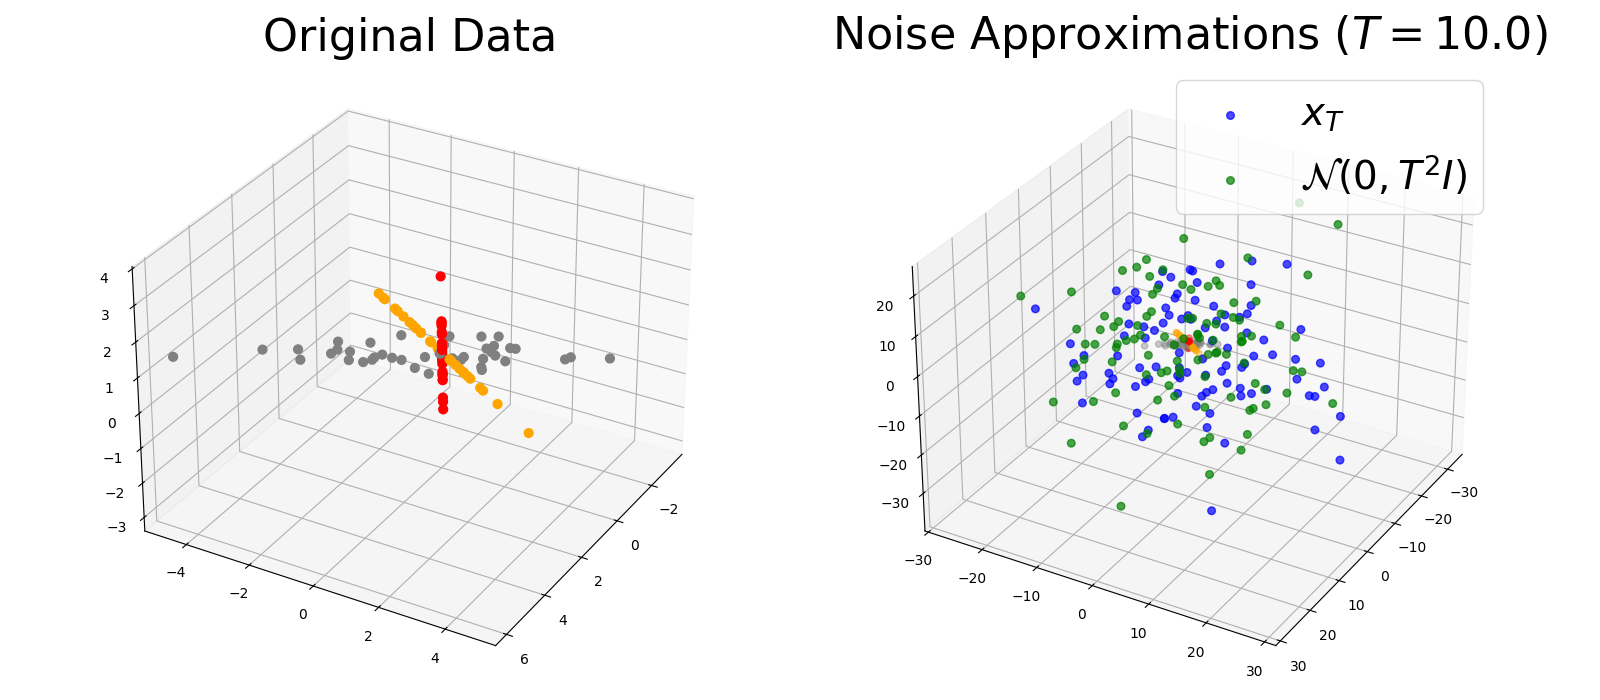
\includegraphics[width=0.75\textwidth]{\toplevelprefix/chapters/chapter3/figs/xT_vs_noise.png}
	\caption{\small\textbf{Vizualizarea \(\vx_{T}\) versus \(\dNorm(\vzero, T^{2}\vI)\).} \textit{Stânga:} O reprezentare grafică a datelor modelului de amestec Gaussian \(\vx\). \textit{Dreapta:} O reprezentare grafică a lui \(\vx\) precum și \(\vx_{T}\) și un eșantion independent de \(\dNorm(\vzero, T^{2}\vI)\), pentru \(T = 10\). Pe graficul din dreapta, \(\vx\) este reprezentat în aceleași culori ca în stânga: cu toate acestea, eșantioanele din \(\vx_{T}\) și \(\dNorm(\vzero, T^{2}\vI)\) sunt ambele mult mai mari, în medie, decât eșantioanele din \(\vx\), și astfel apare mult mai mic din cauza scalării. În ciuda acestei măriri mari, observăm clar similaritățile în distribuțiile lui \(\vx_{T}\) și \(\dNorm(\vzero, T^{2}\vI)\).}
	\label{fig:xT_vs_noise}
\end{figure}

Deci, discretizând \([0, T]\) în \(0 = t_{0} < t_{1} < \cdots < t_{L} = T\) uniform folosind \(t_{\ell} = T\ell / L\) (ca în secțiunea anterioară), o modalitate posibilă de a eșantiona din zgomot pur este:
\begin{itemize}
	\item Eșantionează \(\hat{\vx}_{T} \sim \dNorm(\vzero, T^{2}\vI)\) (i.i.d.~de orice altceva) 
	\item Rulează iterația de îndepărtare a zgomotului ca în \Cref{sub:intro_diffusion_denoising}, adică,
		\begin{equation}\label{eq:denoising-iteration-basic}
		\hat{\vx}_{t_{\ell - 1}} = \bp{1 - \frac{1}{\ell}}\cdot\hat{\vx}_{t_{\ell}} + \frac{1}{\ell}\cdot\bar{\vx}^{\ast}(t_{\ell}, \hat{\vx}_{t_{\ell}}).
	\end{equation}
	\item Returnează \(\hat{\vx} = \hat{\vx}_{0}\).
\end{itemize}
Aceasta este conceptual tot ce stă în spatele \textit{modelelor de difuzie}, care transformă zgomotul în eșantioane de date în conformitate cu primul deziderat. Cu toate acestea, mai sunt câțiva pași de făcut înainte de a obține modele care pot efectiv eșantiona din distribuții de date reale precum imagini, date constrângerile practice de resurse. În continuare, vom introduce și motiva câțiva astfel de pași.

\paragraph{Pasul 1: discretizări diferite.} Primul pas pe care îl facem este motivat de următorul punct: \textit{nu trebuie să cheltuim atât de multe iterații de îndepărtare a zgomotului} la \(t\) mare. Dacă ne uităm la \Cref{fig:ve_gmm_denoising}, observăm că primele \(200\) sau \(300\) de iterații din cele \(500\) de iterații ale procesului de eșantionare sunt cheltuite doar contractând zgomotul către distribuția datelor ca întreg, înainte ca iterațiile rămase să împingă eșantioanele către un subspațiu. Dat un număr fix de iterații \(L\), aceasta semnalează că ar trebui să cheltuim mai mulți pași de timp \(t_{\ell}\) aproape de \(t = 0\) comparativ cu \(t = T\). În timpul eșantionării (și antrenării), putem folosi prin urmare o altă discretizare a \([0, T]\) în \(0 \leq t_{0} < t_{1} < \cdots < t_{L} \leq T\), cum ar fi o \textit{discretizare exponențială}:
\begin{equation}\label{eq:denoising_exponential_discretization}
	t_{\ell} = C_{1}(e^{C_{2}\ell} - 1), \qquad \forall \ell \in \{0, 1, \dots, L\}
\end{equation}
unde \(C_{1}, C_{2} > 0\) sunt constante care pot fi ajustate pentru performanță optimă în practică; analiza teoretică va specifica adesea astfel de constante optime de asemenea. Atunci iterația de îndepărtare a zgomotului/eșantionare devine 
\begin{equation}\label{eq:denoising_iteration}
	\hat{\vx}_{t_{\ell - 1}} \doteq \frac{t_{\ell - 1}}{t_{\ell}}\hat{\vx}_{t_{\ell}} + \bp{1 - \frac{t_{\ell - 1}}{t_{\ell}}}\bar{\vx}^{\ast}(t_{\ell}, \hat{\vx}_{t_{\ell}}),
\end{equation}
cu, din nou, \(\hat{\vx}_{t_{L}} \sim \dNorm(\vzero, t_{L}^{2}\vI)\).

\paragraph{Pasul 2: modele de zgomot diferite.} Al doilea pas este să considerăm modele ușor diferite comparativ cu \eqref{eq:additive_gaussian_noise_model}. Motivația de bază pentru aceasta este următoarea. În practică, distribuția zgomotului \(\dNorm(\vzero, t_{L}^{2}\vI)\) devine o estimare din ce în ce mai slabă a covarianței adevărate în dimensiuni înalte, adică, \eqref{eq:ve_converge_to_large_gaussian} devine o aproximare din ce în ce mai proastă, în special cu date anizotrope cu dimensiuni înalte. Distanța crescută dintre \(\dNorm(\vzero, t_{L}^{2}\vI)\) și distribuția adevărată a lui \(\vx_{t_{L}}\) poate face ca denoiser-ul să funcționeze mai prost în astfel de circumstanțe. Teoretic, \(\vx_{t_{L}}\) nu converge niciodată la nicio distribuție pe măsură ce \(t_{L}\) crește, deci această configurare este dificil de analizat de la cap la coadă. În acest caz, remediul nostru este să \textit{adăugăm simultan zgomot și să micșorăm contribuția lui \(\vx\), astfel încât \(\vx_{T}\) să convergă pe măsură ce \(T \to \infty\)}. Rata de zgomot adăugat este notată \(\sigma \colon [0, T] \to \R_{\geq 0}\), iar rata de micșorare este notată \(\alpha \colon [0, T] \to \R_{\geq 0}\), astfel încât \(\sigma\) este \textit{crescătoare} și \(\alpha\) este (nu strict) \textit{descrescătoare}, și 
\begin{equation}\label{eq:gen_additive_gaussian_noise_model}
	\vx_{t} \doteq \alpha_{t}\vx + \sigma_{t}\vg, \qquad \forall t \in [0, T].
\end{equation}
Configurarea anterioară are \(\alpha_{t} = 1\) și \(\sigma_{t} = t\), și aceasta se numește \textit{procesul cu varianță explozivă (VE)}. O alegere populară care scade contribuția lui \(\vx\), așa cum am descris inițial, are \(T = 1\) (astfel încât \(t \in [0, 1]\)), \(\alpha_{t} = \sqrt{1 - t^{2}}\) și \(\sigma_{t} = t\); acesta este \textit{procesul cu păstrarea varianței (VP)}. Notați că sub procesul VP, \(\vx_{1} \sim \dNorm(\vzero, \vI)\) exact, astfel încât putem eșantiona pur și simplu din această distribuție standard și să îndepărtăm zgomotul iterativ. Ca rezultat, procesul VP este mult mai ușor de analizat teoretic și mai stabil empiric.\footnote{De ce să folosim întreaga configurare \(\alpha, \sigma\)? După cum vom vedea în \Cref{exercise:implement_denoising_processes}, aceasta încapsulează și unifică multe procese propuse, inclusiv procesul recent popular așa-numit \textit{potrivire de flux}. În ciuda acestui fapt, procesele VE și VP sunt încă cele mai populare empiric și teoretic (până acum), și astfel le vom considera în această secțiune.} 

Cu această configurare mai generală, formula lui Tweedie \eqref{eq:tweedie} devine 
\begin{equation}\label{eq:gen_tweedie}
	\Ex[\vx \mid \vx_{t}] = \frac{1}{\alpha_{t}}\bp{\vx_{t} + \sigma_{t}^{2}\nabla \log p_{t}(\vx)}.
\end{equation}
Iterația de îndepărtare a zgomotului \eqref{eq:denoising_iteration} devine
\begin{equation}\label{eq:gen_denoising_iteration}
	\hat{\vx}_{t_{\ell - 1}} = \frac{\sigma_{t_{\ell - 1}}}{\sigma_{t_{\ell}}}\hat{\vx}_{t_{\ell}} + \bp{\alpha_{t_{\ell - 1}} - \frac{\sigma_{t_{\ell - 1}}}{\sigma_{t_{\ell}}}\alpha_{t_{\ell}}}\bar{\vx}^{\ast}(t_{\ell}, \hat{\vx}_{t_{\ell}}).
\end{equation}
În final, denoiser-ul modelului de amestec Gaussian \eqref{eq:gmm_bayes_optimal_denoiser} devine 
\begin{equation}\label{eq:gen_gmm_bayes_optimal_denoiser}
	\bar{\vx}^{\ast}(t, \vx_{t}) = \sum_{k = 1}^{K}\frac{\pi_{k}\phi(\vx_{t} ; \alpha_{t}\boldsymbol{\mu}_{k}, \alpha_{t}^{2}\boldsymbol{\Sigma}_{k} + \sigma_{t}^{2}\vI)}{\sum_{j = 1}^{K}\pi_{j}\phi(\vx_{t} ; \alpha_{t}\boldsymbol{\mu}_{j}, \alpha_{t}^{2}\boldsymbol{\Sigma}_{j} + \sigma_{t}^{2}\vI)}\bp{\boldsymbol{\mu}_{k} + \boldsymbol{\Sigma}_{k}(\alpha_{t}^{2}\boldsymbol{\Sigma}_{k} + \sigma_{t}^{2}\vI)^{-1}(\vx_{t} - \alpha_{t}\boldsymbol{\mu}_{k})}.
\end{equation}

\begin{figure}[!htbp]
	\centering 
	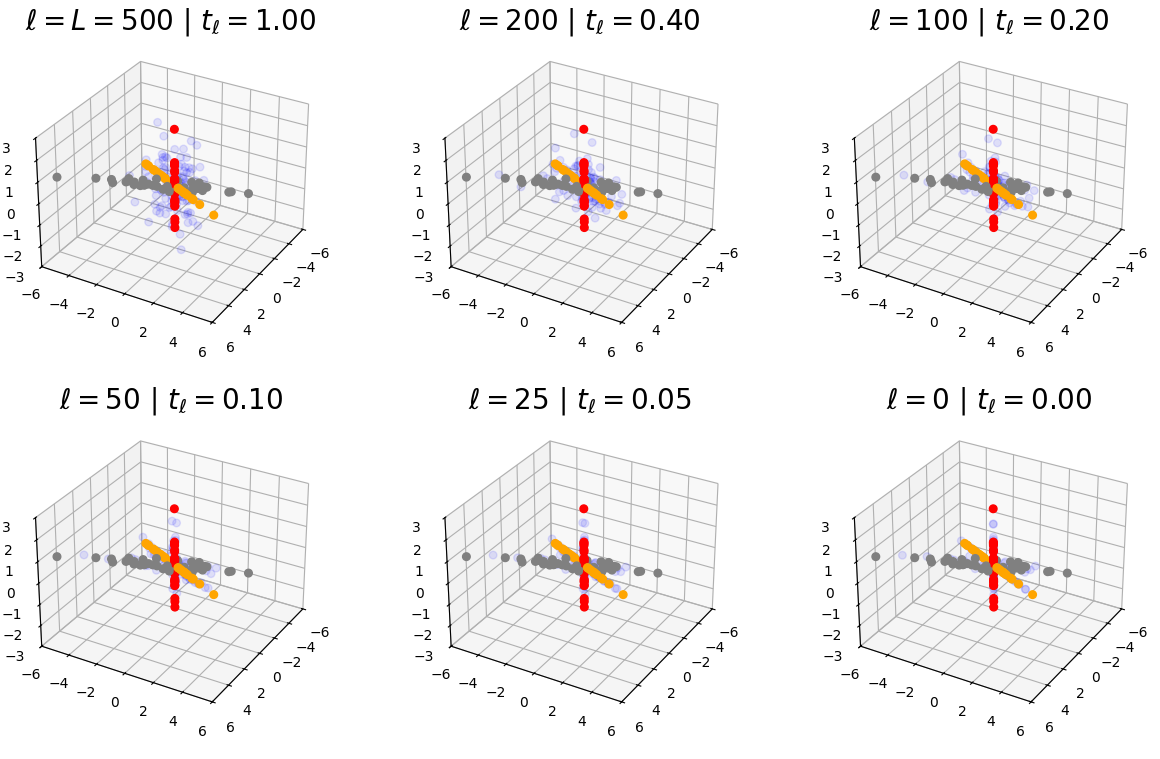
\includegraphics[width=\textwidth]{\toplevelprefix/chapters/chapter3/figs/vp_gmm_denoising.png}
	\caption{\small\textbf{Îndepărtarea zgomotului dintr-un amestec de Gaussiene folosind procesul de difuzie VP.} Folosim aceeași configurare grafică și distribuție de date ca în \Cref{fig:ve_gmm_denoising}. Notați că, comparativ cu \Cref{fig:ve_gmm_denoising}, distribuția zgomotului este mult mai concentrată în jurul originii.}
	\label{fig:vp_gmm_denoising}
\end{figure}

\paragraph{Pasul 3: învățarea unui singur denoiser parametric.} Până acum am presupus că avem denoiser-ul Bayes-optim \(\bar{\vx}^{\ast}(t, \cdot)\) pentru toți \(t\). Dar în practică nu cunoaștem distribuția \(p(\vx)\), deci nu putem calcula \(\bar{\vx}^{\ast}(t, \cdot)\). În schimb, va trebui să \textit{învățăm} denoiser-ul din date. Acest lucru duce la două probleme: (1) cum să învățăm un denoiser și (2) cum să învățăm un denoiser pentru fiecare \(t\). În general, există două abordări. Prima este să antrenăm \(L\) denoisere, unul pentru fiecare pas de timp discret, dar aceasta necesită o cantitate substanțială de memorie și nu generalizează la pași de timp nevăzuți anterior. A doua este să antrenăm un singur denoiser \textit{parametric} (rețea neurală) \(\bar{\vx}_{\theta}(t, \cdot)\) prin optimizare pe spațiul de parametri \(\Theta\) pentru a minimiza eroarea pătratică medie pe toți pașii de timp:
\begin{equation}
	\min_{\theta}\Ex_{t, \vx, \vx_{t}}\norm{\bar{\vx}_{\theta}(t, \vx_{t}) - \vx}_{2}^{2}.
\end{equation}
Similar cu Pasul 1, unde am folosit mai mulți pași de timp aproape de \(t = 0\) pentru a asigura un proces de eșantionare mai bun, am putea dori să ne asigurăm că denoiser-ul este de calitate mai înaltă aproape de \(t = 0\), și astfel să \textit{ponderăm pierderea} astfel încât \(t\) aproape de \(0\) să aibă o pondere mai mare. Fie \(w_{t}\) ponderea la timpul \(t\), pierderea ponderată ar arăta astfel:
\begin{equation}\label{eq:parametric_denoising_loss}
	\min_{\theta}\Ex_{t}w_{t}\Ex_{\vx, \vx_{t}}\norm{\bar{\vx}_{\theta}(t, \vx_{t}) - \vx}_{2}^{2}.
\end{equation}
O alegere rezonabilă de pondere în practică este \(w_{t} = \alpha_{t}/\sigma_{t}\). Motivul precis va fi acoperit în paragraful următor, dar în general servește la creșterea ponderilor pierderilor corespunzătoare lui \(t\) aproape de \(0\), rămânând în același timp rezonabil stabil numeric. De asemenea, desigur, nu putem calcula așteptarea în practică, așa că folosim cea mai simplă medie Monte-Carlo pentru a o estima. Seria de schimbări făcute aici au mai multe beneficii conceptuale și computaționale: nu trebuie să antrenăm mai mulți denoisere, putem antrena pe un set de pași de timp și eșantiona folosind un subset (sau altele complet diferite), etc. Pipeline-ul complet este discutat în \Cref{alg:learning_denoiser}.

\begin{algorithm}
	\begin{algorithmic}[1]
		\Require{Set de date \(\cD \subseteq \R^{D}\).}
		\Require{O listă ordonată de pași de timp \(0 \leq t_{0} < \cdots < t_{L} \leq T\) de folosit pentru eșantionare.}
		\Require{O funcție de ponderare \(w \colon \{t_{\ell}\}_{\ell = 1}^{L} \to \R_{\geq 0}\).}
		\Require{Funcții de scală și nivel de zgomot \(\alpha, \sigma \colon \{t_{\ell}\}_{\ell = 0}^{L} \to \R_{\geq 0}\).}
		\Require{Un spațiu de parametri \(\Theta\) și o arhitectură de denoiser \(\bar{\vx}_{\theta}\).}
		\Require{Un algoritm de optimizare pentru parametri.}
		\Require{Numărul de iterații de optimizare \(M\).}
		\Require{Numărul de extrageri Monte-Carlo \(N\) pe iterație (pentru a aproxima așteptarea în \eqref{eq:parametric_denoising_loss}).}
		\Ensure{Un denoiser antrenat \(\bar{\vx}_{\theta^{\ast}}\).}

		\Function{AntreneazăDenoiser}{$\cD, \Theta$}
		\State{Inițializează \(\theta^{(1)} \in \Theta\)}
		\For{\(i \in [M]\)}
		\For{\(n \in [N]\)}
		\State{\(\vx_{n}^{(i)} \sim \cD\)} \Comment{Extrage un eșantion din setul de date.}
		\State{\(t_{n}^{(i)} \simiid \dUnif(\{t_{\ell}\}_{\ell = 1}^{L})\)} \Comment{Eșantionează un pas de timp.}
		\State{\(\vg_{n}^{(i)} \simiid \dNorm(\vzero, \vI)\)} \Comment{Eșantionează un vector de zgomot.}
		\State{\(\vx_{t, n}^{(i)} \doteq \alpha_{t_{n}^{(i)}}\vx_{n}^{(i)} + \sigma_{t_{n}^{(i)}}\vg_{n}^{(i)}\)} \Comment{Calculează eșantionul cu zgomot.}
		\State{\(w_{n}^{(i)} \doteq w_{t_{n}^{(i)}}\)} \Comment{Calculează ponderea pierderii.}
		\EndFor
		\State{\(\hat{\cL}^{(i)} \doteq \displaystyle \frac{1}{N}\sum_{n = 1}^{N}w_{n}^{(i)}\norm{\vx_{n}^{(i)} - \bar{\vx}_{\theta^{(i)}}(t_{n}^{(i)}, \vx_{t, n}^{(i)})}_{2}^{2}\)} \Comment{Calculează estimarea pierderii.}
		\State{\(\theta^{(i + 1)} \doteq \texttt{ActualizareOptimizare}^{(i)}(\theta^{(i)}, \nabla_{\theta^{(i)}}\hat{\cL}^{(i)})\)} \Comment{Actualizează parametrii.}
		\EndFor
		\State{\Return{\(\bar{\vx}_{\theta^{(K + 1)}}\)}}
		\EndFunction
	\end{algorithmic}
	\caption{Învățarea unui denoiser din date.}
	\label{alg:learning_denoiser}
\end{algorithm}

\begin{algorithm}
	\caption{Eșantionare folosind un denoiser.}
	\label{alg:iterative_denoising}
	\begin{algorithmic}[1]
		\Require{O listă ordonată de pași de timp \(0 \leq t_{0} < \cdots < t_{L} \leq T\) de utilizat pentru eșantionare.}
		\Require{Un denoiser \(\bar{\vx} \colon \{t_{\ell}\}_{\ell = 1}^{L} \times \R^{D} \to \R^{D}\).}
		\Require{Funcții de scală și nivel de zgomot \(\alpha, \sigma \colon \{t_{\ell}\}_{\ell = 0}^{L} \to \R_{\geq 0}\).}
		\Ensure{Un eșantion \(\hat{\vx}\), aproximativ din distribuția lui \(\vx\).}
		\Function{DDIMSampler}{$\bar{\vx}, (t_{\ell})_{\ell = 0}^{L}$}
		\State{Inițializează \(\tilde{\vx}_{t_{L}} \sim\) distribuția aproximativă a lui \(\vx_{t_{L}}\)} \Comment{VP \(\implies \dNorm(\vzero, \vI)\), VE \(\implies \dNorm(\vzero, t_{L}^{2}\vI)\).}
		\For{\(\ell = L, L - 1, \dots, 1\)}
		\State{Calculează
			\begin{equation*}
				\hat{\vx}_{t_{\ell - 1}} \doteq \frac{\sigma_{t_{\ell - 1}}}{\sigma_{t_{\ell}}}\hat{\vx}_{t_{\ell}} + \bp{\alpha_{t_{\ell - 1}} - \frac{\sigma_{t_{\ell - 1}}}{\sigma_{t_{\ell}}}\alpha_{t_{\ell}}}\bar{\vx}(t_{\ell}, \hat{\vx}_{t_{\ell}})
			\end{equation*}
		}
		\EndFor
		\State{\Return{\(\hat{\vx}_{t_{0}}\)}}
		\EndFunction
	\end{algorithmic}
\end{algorithm}

\paragraph{(Opțional) Pasul 4: schimbarea țintei de estimare.} Notați că este comun să reorientăm întreaga conductă de îndepărtare a zgomotului în jurul \textit{predictorilor de zgomot}, adică, estimări ale \(\Ex[\vg \mid \vx_{t}]\). În practică, predictorii de zgomot sunt ușor mai ușor de antrenat deoarece ieșirea lor este (aproape) întotdeauna de dimensiune comparabilă cu o variabilă aleatoare Gaussiană, astfel încât antrenarea este mai stabilă numeric. Notați că prin \eqref{eq:gen_additive_gaussian_noise_model} avem 
\begin{equation}
	\vx_{t} = \alpha_{t}\Ex[\vx \mid \vx_{t}] + \sigma_{t}\Ex[\vg \mid \vx_{t}] \implies \Ex[\vg \mid \vx_{t}] = \frac{1}{\sigma_{t}}\bp{\vx_{t} - \alpha_{t}\Ex[\vx \mid \vx_{t}]},
\end{equation}
Prin urmare, orice predictor pentru \(\vx\) poate fi transformat într-un predictor pentru \(\vg\) folosind relația de mai sus, adică,
\begin{equation}
	\bar{\vg}(t, \vx_{t}) = \frac{1}{\sigma_{t}}\vx_{t} - \frac{\alpha_{t}}{\sigma_{t}}\bar{\vx}(t, \vx_{t}),
\end{equation}
și vice-versa. Astfel, o rețea bună pentru estimarea \(\bar{\vg}\) este aceeași cu o rețea bună pentru estimarea \(\bar{\vx}\) \textit{plus o conexiune reziduală} (așa cum se vede în, de exemplu, transformatoare). Pierderile lor sunt de asemenea aceleași ca denoiser-ul, până la factorul de \(\alpha_{t}/\sigma_{t}\).

\paragraph{Convergența procesului de eșantionare.} Acum că am dezvoltat procesul de eșantionare prin difuzie, este natural să ne întrebăm cât de bine funcționează. Pentru a măsura acuratețea eșantionării, folosim \textit{distanța de variație totală} (TV) între distribuția adevărată \(\vx\) și distribuția eșantionată \(\hat{\vx}\):
\begin{equation}
	\TV(\vx, \vy) \doteq \sup_{A \subseteq \R^{d}}\abs*{\Pr[\vx \in A] - \Pr[\vy \in A]}.
\end{equation}
Dacă \(\vx\) și \(\vy\) sunt foarte aproape (uniform), atunci supremumul va fi mic. Deci distanța TV măsoară apropierea variabilelor aleatoare. (Este într-adevăr o metrică, după cum sugerează numele; demonstrația este un exercițiu.)

\begin{theorem}[\citep{li2024d} Teorema 1, Simplificată]\label{thm:diffusion_sampler_convergence}
	Să presupunem că \(\Ex\norm{\vx}_{2} < \infty\). Dacă \(\vx\) este denoised conform procesului VP cu o discretizare exponențială\footnote{Definiția precisă este destul de lungă în notația noastră și definită doar până la diverse constante absolute, așa că o omitem aici pentru concizie. Desigur, este în lucrarea originală \citep{li2024d}.} ca în \eqref{eq:denoising_exponential_discretization}, ieșirea \(\hat{\vx}\) a \Cref{alg:iterative_denoising} satisface limita de variație totală
	\begin{equation}\label{eq:diffusion_sampling_error}
		\TV(\vx, \hat{\vx}) = \tilde{\cO}\rp{\underbrace{\frac{D}{L}}_{\text{eroare de discretizare}} + \underbrace{\sqrt{\frac{1}{L}\sum_{\ell = 1}^{L}\frac{\alpha_{t_{\ell}}}{\sigma_{t_{\ell}}^{2}}\Ex_{\vx, \vx_{t_{\ell}}}\norm{\bar{\vx}^{\ast}(t_{\ell}, \vx_{t_{\ell}}) - \bar{\vx}(t_{\ell}, \vx_{t_{\ell}})}_{2}^{2}}}_{\text{eroare medie în exces a denoiser-ului}}}
	\end{equation}
	unde \(\bar{\vx}^{\ast}\) este denoiser-ul Bayes optimal pentru \(\vx\), și \(\tilde{\cO}\) este o versiune a notației big-\(\cO\) care ignoră factorii logaritmici în \(L\).
\end{theorem}
Tehnica de demonstrație la nivel foarte înalt este, așa cum s-a discutat mai devreme, să limităm eroarea la fiecare pas, să distingem sursele de eroare (între discretizare și eroarea denoiser-ului) și să ne asigurăm cu grijă că erorile nu se acumulează prea mult (sau chiar se anulează).

Notați că dacă \(L \to \infty\) și învățăm corect denoiser-ul Bayes optimal \(\bar{\vx} = \bar{\vx}^{\ast}\) (astfel încât eroarea în exces să fie \(0\)), atunci procesul de eșantionare din \Cref{alg:iterative_denoising} produce o \textit{inversă perfectă (în distribuție)} a procesului de adăugare a zgomotului, deoarece rata de eroare din \Cref{thm:diffusion_sampler_convergence} merge la \(0\),\footnote{Există rezultate similare pentru procesele VE, deși niciunul nu este la fel de precis ca acesta după cunoștințele noastre.} așa cum s-a argumentat euristic anterior.

\begin{remark}
	Ce se întâmplă dacă datele sunt cu dimensiuni reduse, să zicem susținute pe un \textit{subspațiu de rang redus} al spațiului cu dimensiuni înalte \(\R^{D}\)? Dacă distribuția datelor are suport compact---să zicem dacă datele sunt normalizate la hipercubul unitar, ceea ce este adesea asigurat ca un pas de pre-procesare pentru date reale precum imagini---este posibil să obținem rezultate mai bune. Mai exact, autorii \cite{li2024d} definesc de asemenea o măsură de \textit{dimensiune intrinsecă aproximativă} folosind asimptoticele așa-numitului număr de acoperire, care este extrem de similar în intuiție (dacă nu în implementare) cu funcția ratei distorsiunii prezentată în următoarea Secțiune. Apoi ei arată că folosind o modificare mică particulară a eșantionatorului DDIM din \Cref{alg:iterative_denoising} (i.e., perturbând ușor coeficienții de actualizare), eroarea de discretizare devine
	\begin{equation}
		\tilde{\cO}\rp{\frac{\text{dimensiune intrinsecă aproximativă}}{L}}
	\end{equation}
	în loc de \(\frac{D}{L}\) cum era în \Cref{thm:diffusion_sampler_convergence}. Prin urmare, folosind acest algoritm modificat, \(L\) nu trebuie să fie prea mare chiar și când \(D\) ajunge la mii sau milioane, deoarece datele reale au structură cu dimensiuni reduse. Cu toate acestea, în practică folosim eșantionatorul DDIM în schimb, așa că \(L\) ar trebui să aibă o dependență ușoară de \(D\) pentru a obține rate de eroare consistente. Alegerea exactă a lui \(L\) face un compromis între complexitatea computațională (de exemplu, timpul de execuție sau consumul de memorie) al eșantionării și complexitatea statistică a învățării unui denoiser pentru structuri cu dimensiuni reduse. Valoarea lui \(L\) este adesea diferită la timpul de antrenare (unde un \(L\) mai mare permite o acoperire mai bună a intervalului \([0, T]\), ceea ce ajută rețeaua să învețe o relație care generalizează peste \(t\)) și timpul de eșantionare (unde \(L\) fiind mai mic înseamnă eșantionare mai eficientă). Se pot chiar alege pașii de timp adaptiv la timpul de eșantionare pentru a optimiza aceste compromisuri \cite{bao2022analytic}.
\end{remark}

\begin{remark}
	Diverse alte lucrări definesc procesul invers ca mișcându-se înapoi în indexul de timp \(t\) folosind o ecuație cu diferențe explicită, sau ecuație diferențială în limita \(L \to \infty\), sau înainte în timp folosind transformarea \(\vy_{t} = \vx_{T - t}\), astfel încât dacă \(t\) crește atunci \(\vy_{t}\) devine mai aproape de \(\vx_{0}\). În această lucrare ne străduim să păstrăm consistența: ne mișcăm înainte în timp pentru a adăuga zgomot și înapoi în timp pentru a îndepărta zgomotul. Dacă citiți o altă lucrare care nu este clară cu privire la indexul de timp, sau încercați să implementați un algoritm care este similar neclar, există o modalitate de a face acest lucru corect de fiecare dată: procesul de eșantionare ar trebui să aibă întotdeauna un coeficient \textit{pozitiv} atât pe termenul denoiser-ului, cât și pe iterația curentă când se trece de la pas la pas. Dar în general multe lucrări își definesc propria notație și nu este prietenoasă cu utilizatorul.
\end{remark}

\begin{remark}
	Teoria prezentată la sfârșitul ultimei \Cref{sub:intro_diffusion_denoising} pare să sugereze (vorbind liber) că în practică, folosirea unei rețele de tip transformer este o alegere bună pentru învățarea sau aproximarea unui denoiser. Acest lucru este rezonabil, dar care este problema cu utilizarea oricărei rețele neuronale vechi (cum ar fi un perceptron multistrat (MLP)) și doar încercarea de a o scala la infinit? Pentru a observa problema cu aceasta, să ne uităm la un alt caz special al modelului de amestec gaussian studiat în \Cref{example:denoising_gaussian_mixture}. Mai exact, \textit{distribuția empirică} este o instanță a unui model de amestec gaussian degenerat, cu \(K = N\) componente \(\dNorm(\vx_{i}, \vzero)\) eșantionate cu probabilitate egală \(\pi_{i} = \frac{1}{N}\). În acest caz, denoiser-ul Bayes optimal este
	\begin{equation}\label{eq:memorizing_denoiser}
		\bar{\vx}^{\star}(t, \vx_{t}) = \sum_{i = 1}^{N}\frac{e^{-\|\vx_{t} - \alpha_{t}\vx_{i}\|_{2}^{2}/(2\sigma_{t}^{2})}}{\sum_{j = 1}^{N}e^{-\|\vx_{t} - \alpha_{t}\vx_{j}\|_{2}^{2}/(2\sigma_{t}^{2})}}\vx_{i}.
	\end{equation}
	Aceasta este o combinație convexă a datelor \(\vx_{i}\), și coeficienții devin „mai ascuțiți" (i.e., mai aproape de \(0\) sau \(1\)) pe măsură ce \(t \to 0\). Observați că acest denoiser \textit{rezolvă optimal} problema de optimizare a îndepărtării zgomotului \eqref{eq:parametric_denoising_loss} când calculăm pierderea pe baza extragerii lui \(\vx\) uniform aleator dintr-un set de date finit fix \(\vX = \{\vx_{i}\}_{i = 1}^{N}\), care este o setare foarte realistă. Astfel, dacă arhitectura noastră de rețea \(\bar{\vx}_{\theta}\) este suficient de expresivă astfel încât denoiserii optimi de forma de mai sus \eqref{eq:memorizing_denoiser} pot fi bine aproximați, atunci denoiser-ul învățat poate face exact asta. Apoi, îndepărtarea noastră iterativă a zgomotului \Cref{alg:iterative_denoising} va eșantiona exact din distribuția empirică, re-generând eșantioane din datele de antrenare, așa cum este certificat de \Cref{thm:diffusion_sampler_convergence}. Acesta este un eșantionator prost, nu cu adevărat mai interesant decât o bază de date cu toate eșantioanele, și astfel este important să înțelegem cum să evităm acest lucru în practică. Cheia este să venim cu o arhitectură de rețea care poate aproxima bine denoiser-ul adevărat (să zicem corespunzător unei distribuții de rang redus ca în \eqref{eq:gmm_lowrank_denoiser}) dar nu denoiser-ul bayesian empiric ca în \eqref{eq:memorizing_denoiser}. Unele lucrări au explorat această linie fină și de ce modelele de difuzie moderne, care folosesc arhitecturi de rețea bazate pe transformatoare și convoluționale, pot memoriza și generaliza în regimuri diferite \citep{kamb2024analytic,niedoba2024towards}.

	La un nivel înalt, un denoiser care memorează toate punctele de antrenare, ca în \eqref{eq:memorizing_denoiser}, corespunde unui model parametric al distribuției care are rata de codificare minimă și obține aceasta prin codificarea fiecărui eșantion separat. Vom discuta această problemă (și paradoxul aparent cu dezideratele noastre inițiale la sfârșitul \Cref{sub:min_entropy}) din perspectiva teoriei informației în următoarea secțiune.
\end{remark}

Am făcut multe modificări procesului nostru platonic original de adăugare/îndepărtare a zgomotului. Pentru a ne asigura că noul proces funcționează încă în practică, putem calcula exemple numerice (cum ar fi \Cref{fig:vp_gmm_denoising}). Pentru a ne asigura că este solid din punct de vedere teoretic, putem demonstra o \textit{limită a ratei de eroare} pentru algoritmul de eșantionare, care arată că rata de eroare este mică. Vom furniza acum o astfel de rată din literatură, care arată că distribuția de ieșire a eșantionatorului converge în așa-numita \textit{distanță de variație totală (TV)} către distribuția adevărată. Distanța TV este definită între două variabile aleatoare \(\vx\) și \(\vy\) ca:
\begin{equation}
	\TV(\vx, \vy) \doteq \sup_{A \subseteq \R^{d}}\abs*{\Pr[\vx \in A] - \Pr[\vy \in A]}.
\end{equation}
Dacă \(\vx\) și \(\vy\) sunt foarte aproape (uniform), atunci supremumul va fi mic. Deci distanța TV măsoară apropierea variabilelor aleatoare. (Este într-adevăr o metrică, după cum sugerează numele; demonstrația este un exercițiu.)

\section{Compresie prin Codificare cu Pierderi} \label{sec:lossy_compression}

Să recapitulăm ce am acoperit până acum. Am discutat cum să potrivim un \textit{denoiser} \(\bar{\vx}_{\theta}\) folosind eșantioane finite. Am arătat că acest denoiser codifică o distribuție prin faptul că este direct conectat la log-densitatea sa prin formula lui Tweedie \eqref{eq:tweedie}. Apoi, l-am folosit pentru a transforma treptat o distribuție de zgomot pur (entropie mare) către distribuția învățată prin \textit{îndepărtarea iterativă a zgomotului}. Astfel, am dezvoltat primul mod de a învăța sau urmări o distribuție prezentat la sfârșitul \Cref{sub:min_entropy}.

Cu toate acestea, în această metodologie, codificarea distribuției este implicită în forma funcțională a denoiser-ului și parametrii săi, dacă există. De fapt, cititorii atenți ar fi observat că pentru o distribuție generală, nu am specificat niciodată explicit care este forma funcțională pentru denoiser. În practică, oamenii îl modelează de obicei printr-o rețea neurală profundă cu o arhitectură proiectată empiric. În plus, deși știm că procesul de îndepărtare a zgomotului de mai sus reduce entropia, nu știm cu cât, nici nu știm entropia distribuțiilor intermediare și rezultate.

Amintiți-vă că scopul nostru general este să modelăm date dintr-o distribuție (continuă) cu un suport cu dimensiuni reduse. Dacă scopul nostru este să identificăm cel mai „simplu" model care generează datele, s-ar putea considera trei măsuri tipice de parcimonitate: dimensiunea, volumul sau entropia (diferențială). Ei bine, dacă cineva folosește dimensiunea, atunci în mod evident cel mai bun model pentru un set de date dat este distribuția empirică însăși, care este zero-dimensională. Pentru toate distribuțiile cu suporturi cu dimensiuni reduse, entropia diferențială este întotdeauna minus infinit; volumul suporturilor lor este întotdeauna zero. Deci, printre toate distribuțiile cu suporturi cu dimensiuni reduse care ar fi putut genera aceleași eșantioane de date, cum putem decide care este mai bună pe baza acestor măsuri de parcimonitate care nu pot distinge deloc între modelele cu dimensiuni reduse? Această secțiune își propune să abordeze această situație aparent derutantă.

În restul acestui capitol, discutăm un cadru care ne permite să atenuăm dificultatea tehnică de mai sus asociind distribuția învățată cu o schemă explicită calculabilă de codificare și decodificare, urmând a doua abordare sugerată la sfârșitul \Cref{sub:min_entropy}. După cum vom vedea, o astfel de abordare ne permite în esență să aproximăm cu precizie entropia distribuțiilor învățate în termeni de lungime (cu pierderi) de codificare sau rata de codificare asociată cu schema de codificare. Cu o astfel de măsură, nu numai că putem măsura cu precizie cu cât este redusă entropia, prin urmare informația câștigată, prin orice procesare (inclusiv îndepărtarea zgomotului) a distribuției, dar putem deriva și o formă explicită a operatorului optim care poate conduce astfel de operații în modul cel mai eficient. După cum vom vedea în următorul \Cref{ch:representation}, aceasta va duce la o explicație principială pentru arhitectura rețelelor profunde, precum și la proiectări mai eficiente de arhitecturi profunde.

\subsection{Necesitatea Codificării cu Pierderi}

Am discutat anterior, de mai multe ori, o dificultate: dacă învățăm distribuția din eșantioane finite în final, și clasa noastră de funcții de denoisere conține suficiente funcții, cum ne asigurăm că eșantionăm din distribuția \textit{adevărată} (cu suporturi cu dimensiuni reduse), în loc de orice altă distribuție care ar putea produce acele eșantioane finite cu probabilitate mare? Să dezvăluim câteva dintre dificultățile conceptuale și tehnice cu câteva exemple concrete.

\begin{example}[Volum, Dimensiune și Entropie]\label{eg:measures-of-complexity}
Pentru exemplul prezentat în partea de sus a \Cref{fig:1d-line}, să presupunem că am luat câteva eșantioane dintr-o distribuție uniformă pe o linie (să zicem într-un plan 2D). Volumul liniei sau al seturilor de eșantioane este zero.
Geometric, distribuția empirică pe setul finit de eșantioane produs este {\em cea cu dimensiune minimă} care poate produce setul finit de eșantioane.\footnote{Un set de eșantioane discrete sunt toate de dimensiune zero, în timp ce linia de suport este de dimensiune unu.} Dar aceasta pare în contrast cu încă o altă măsură a complexității: entropia. Entropia (diferențială) a liniei este minus infinit, dar entropia (discretă) a acestui set de eșantioane este finită și pozitivă. Deci pare să avem o situație paradoxală conform acestor măsuri comune de parcimonitate sau complexitate: ele nu pot diferenția corect între (modele pentru) distribuții cu suporturi cu dimensiuni reduse deloc, iar unele par să le diferențieze chiar în moduri exact opuse.\footnote{Desigur, strict vorbind, entropia diferențială și entropia discretă nu sunt direct comparabile.}
\end{example}

\begin{example}[Densitate]\label{eg:density} Considerați cele două seturi de puncte de date eșantionate prezentate în \Cref{fig:1d-line}. Geometric, ele sunt în esență aceleași: fiecare set constă din opt puncte și fiecare punct a apărut cu frecvență egală $1/8$. Singura diferență este că pentru al doilea set de date, unele puncte sunt suficient de „apropiate" pentru a fi văzute ca având o densitate mai mare în jurul „clusterului" lor respectiv. Care este mai relevant pentru distribuția adevărată care ar fi putut genera eșantioanele? Cum putem reconcilia o astfel de ambiguitate în interpretarea acestui tip de distribuții (empirice)?
\begin{figure}[t]
	\centering
	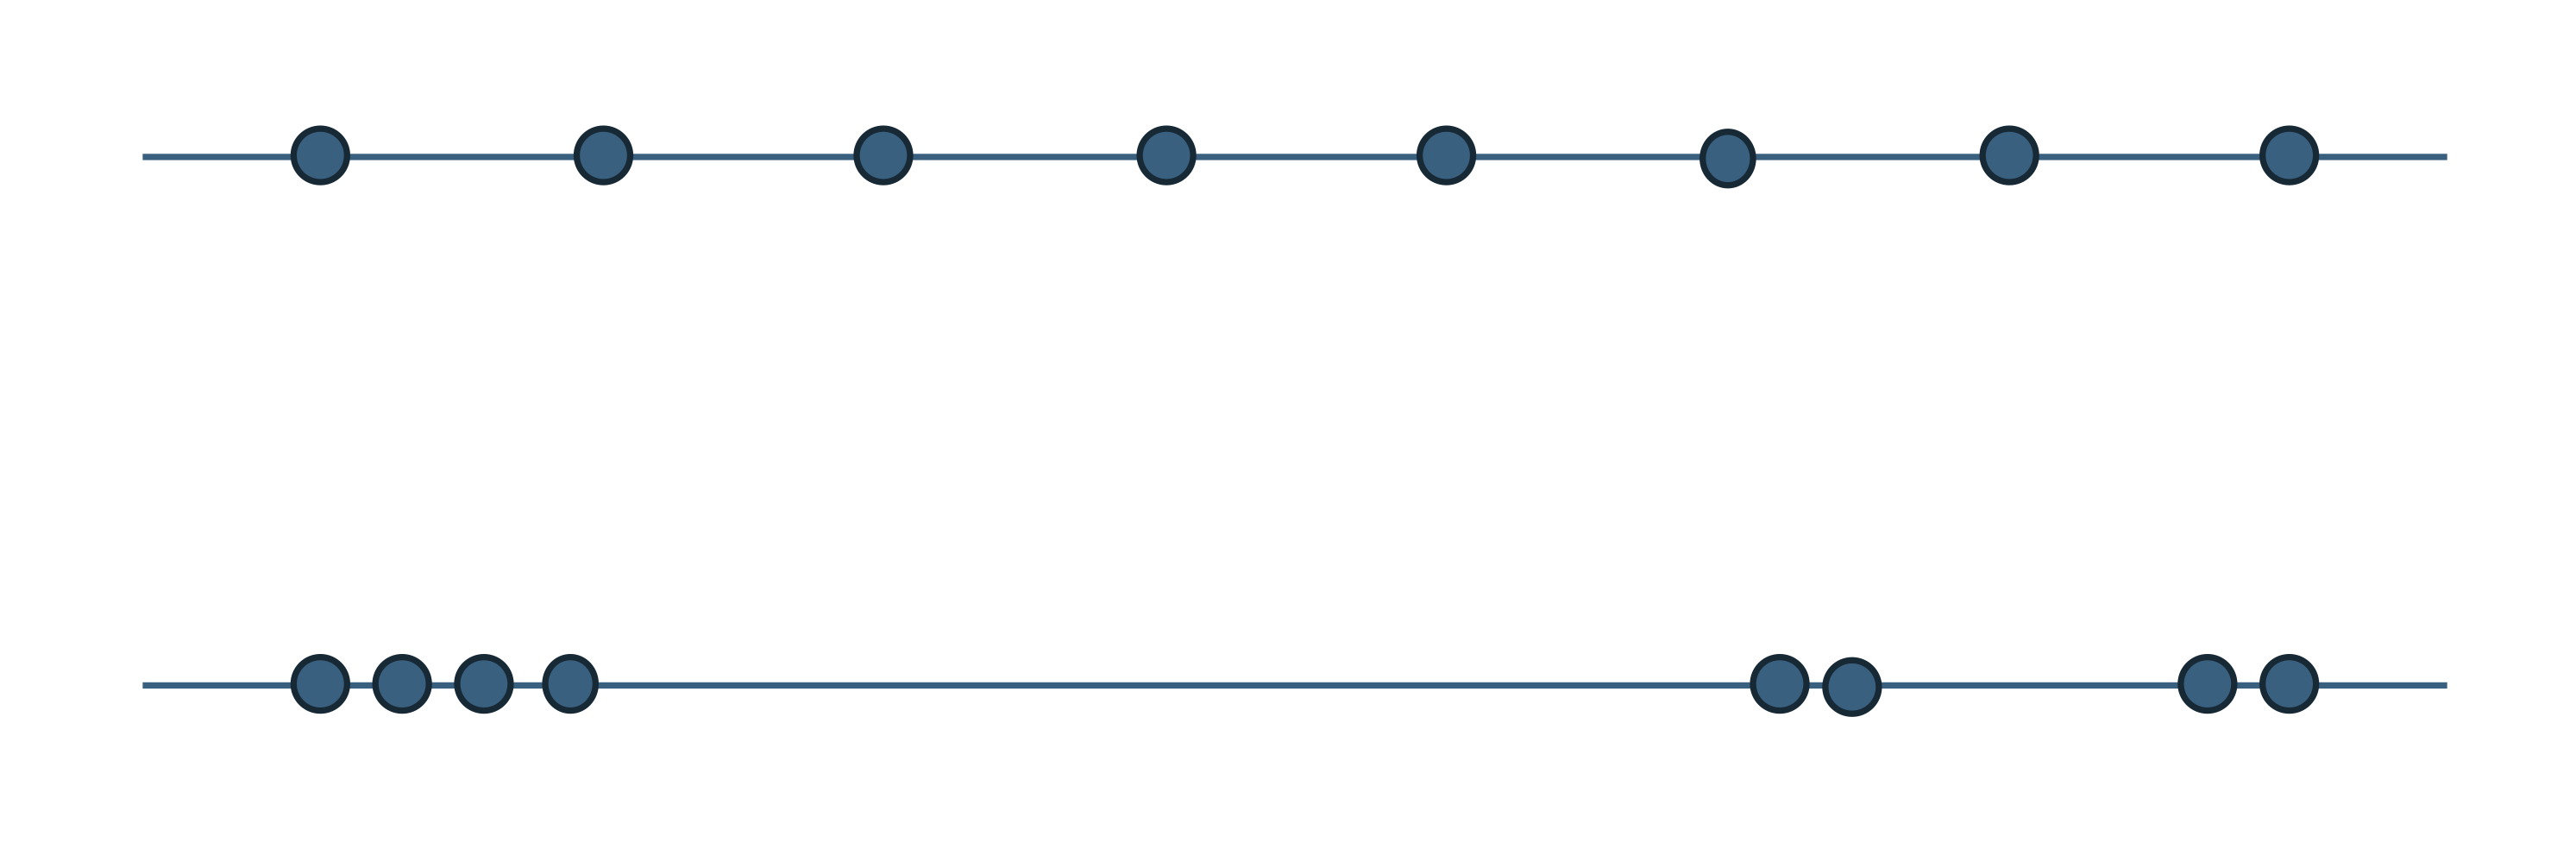
\includegraphics[width=0.7\linewidth]{\toplevelprefix/chapters/chapter3/figs/one-dim-distribution.png}
	\caption{Opt puncte observate pe o linie.}
	\label{fig:1d-line}
\end{figure}
\end{example}

Există încă o altă dificultate tehnică asociată cu construirea unei scheme explicite de codificare și decodificare pentru un set de date. Dat un set de date eșantionate în $\X = [\vx_1, \ldots, \vx_N]$, cum să proiectăm o schemă de codificare care este implementabilă pe mașini cu memorie și resurse de calcul finite? Observați că până și reprezentarea unui număr real general necesită un număr infinit de cifre sau biți. Prin urmare, cineva s-ar putea întreba dacă entropia unei distribuții este o măsură directă pentru complexitatea schemei sale (optime) de codificare. Examinăm această chestiune cu un alt exemplu simplu.

\begin{example}[Precizie] \label{eg:two-inrational}
	Considerați o distribuție discretă $\X = [e, \pi]$ cu probabilitate egală $1/2$ luând valorile numărului lui Euler $e \approx 2.71828$ sau numărul $\pi \approx 3.14159$. Entropia acestei distribuții este $H =1$, ceea ce sugerează că cineva ar putea codifica cele două numere printr-o cifră de un bit $0$ sau $1$, respectiv. Dar puteți realiza o schemă de decodificare pentru acest cod pe o mașină cu stări finite? Răspunsul este de fapt nu, deoarece sunt necesari infinit de mulți biți pentru a descrie oricare dintre numere cu precizie.
\end{example}

Prin urmare, este în general imposibil să avem o schemă de codificare și decodificare care poate reproduce cu precizie eșantioane dintr-o distribuție cu valori reale arbitrare.\footnote{Adică, dacă cineva vrea să codifice astfel de eșantioane cu precizie, singura modalitate este să memoreze fiecare eșantion individual.} Dar ar fi de puțină valoare practică să codificăm o distribuție fără a putea decodifica pentru eșantioane extrase din aceeași distribuție.

Deci pentru a ne asigura că orice schemă de codificare/decodificare este calculabilă și implementabilă cu memorie și resurse computaționale finite, trebuie să cuantificăm eșantionul $\x$ și să-l codificăm doar până la o anumită precizie, să zicem $\epsilon > 0$. {\em Făcând acest lucru, în esență, tratăm orice două puncte de date ca echivalente dacă distanța lor este mai mică de $\epsilon$.} Mai precis, am dori să considerăm scheme de codificare
\begin{equation}
	\x \mapsto \hat \x
\end{equation}
astfel încât eroarea așteptată cauzată de cuantizare să fie mărginită de $\epsilon$. Este matematic mai convenabil și conceptual aproape identic să mărginim eroarea \textit{pătrată} așteptată cu \(\epsilon^{2}\), i.e.,
\begin{equation}
	\Ex[d(\vx, \hat \vx)^{2}] \le \epsilon^{2}.
\end{equation}
De obicei, distanța \(d\) este aleasă să fie distanța euclidiană, sau norma 2.\footnote{Mai general, putem înlocui \(d^{2}\) cu orice așa-numită \textit{divergență}.} Vom adopta această alegere în continuare.

\subsection{Rata Distorsiunii și Geometria Datelor}
Desigur, dintre toate schemele de codificare care satisfac constrângerea de mai sus, am dori să alegem pe cea care minimizează rata de codificare rezultată. Pentru o variabilă aleatoare dată $\x$ și o precizie $\epsilon$, această rată este cunoscută ca {\em rata distorsiunii}, notată ca $\cR_{\epsilon}(\x)$.
O teoremă profundă în teoria informației, demonstrată inițial de \textcite{shannon1959coding}, stabilește că această rată poate fi exprimată echivalent în termeni pur probabilistici ca
\begin{equation}
	\cR_{\epsilon}(\x) 
	= \min_{p(\hat \x \mid \x): \Ex[\norm{\x -\hat \x}_2^{2}] \le \epsilon^{2}} 
	I(\vx; \hat{\vx}),
    \label{eqn:rate-distortion-general}
\end{equation}
unde cantitatea $I(\vx; \hat{\vx})$ este cunoscută ca \textit{informația mutuală}, definită de
\begin{equation}\label{eq:mutual-information}
	I(\vx; \hat{\vx})
	= \KL(p(\vx, \hat{\vx}) \mmid p(\vx) p(\hat{\vx})).
\end{equation}
Observați că minimizarea în \eqref{eqn:rate-distortion-general} este peste toate distribuțiile condiționate $p(\hat \x \mid \x)$ care satisfac constrângerea de distorsiune $\Ex_{\x, \hat \x}[\norm{\x- \hat \x}_2^{2}] \le \epsilon^{2}$.
Fiecare astfel de distribuție condiționată induce o distribuție comună $p(\vx, \hat{\vx}) = p(\hat\x \mid \x) p(\x)$, care determină informația mutuală \eqref{eq:mutual-information}.
Multe proprietăți convenabile ale informației mutuale (și prin urmare rata distorsiunii) sunt implicate de proprietățile corespunzătoare ale divergenței KL (amintiți-vă \Cref{thm:information-inequality}).
Din definiție, știm că $\cR_{\epsilon}(\x)$ este o funcție {\em nedescrescătoare} în $\epsilon$.

\begin{remark}
	În timp ce este posibil să ne așteptăm că rata distorsiunii să fie o aproximare implementabilă a entropiei lui $\x$ în următorul sens. Presupunem că $\vx$ și $\hat{\vx}$ sunt vectori aleatori continui. Atunci informația mutuală poate fi scrisă ca
	\begin{equation}\label{eq:information-entropy}
		I(\x; \hat\x) = h(\x) - h(\x \mid \hat \x),
	\end{equation}
	unde $h(\x \mid \hat \x) = \bE[\log_2 p(\x \mid \hat\x)]$ este \textit{entropia condiționată} a lui $\x$ dată $\hat \x$.
	Prin urmare, rata minimă de codificare este atinsă când diferența dintre entropia lui $\x$ și entropia condiționată a lui $\x$ dată $\hat \x$ este minimizată printre toate distribuțiile care satisfac constrângerea: $\mathbb{E} [\norm{\x- \hat \x}_2^2] \le \epsilon^2$.

	De fapt, nu este necesar să presupunem că $\x$ și $\hat \x$ sunt continue pentru a obține tipul de mai sus de concluzie. De exemplu, dacă ambii vectori aleatori sunt în schimb discreți, avem după o interpretare adecvată a divergenței KL pentru vectori aleatori cu valori discrete că
	\begin{equation}
		I(\x; \hat\x) = H(\x) - H(\x \mid \hat \x).
	\end{equation}
	Mai general, noțiuni matematice avansate din teoria măsurii pot fi folosite pentru a defini informația mutuală (și prin urmare rata distorsiunii) pentru variabile aleatoare arbitrare $\x$ și $\hat \x$, inclusiv cele cu distribuții cu dimensiuni reduse destul de exotice; vezi \textcite[\S 8.5]{Cover-Thomas}.
\end{remark}

\begin{remark}
    Dat un set de puncte de date în $\X = [\x_1,\ldots, \x_N]$, se poate întotdeauna interpreta ca eșantioane dintr-o distribuție discretă uniformă cu probabilitate egală $1/N$ pe acești $N$ vectori. Entropia pentru o astfel de distribuție este $H(\X) = \frac{1}{N}\log_2 N$.\footnote{Observați din nou, chiar dacă putem codifica acești vectori cu această rată de codificare, nu îi putem decodifica cu o precizie arbitrară.} Cu toate acestea, chiar dacă $\X$ este o distribuție uniformă pe eșantioanele sale, rata de codificare $\cR_{\epsilon}(\X)$ realizabilă cu o schemă de codificare cu pierderi ar putea fi semnificativ mai mică decât $H(\X)$ dacă aceste eșantioane nu sunt atât de uniform distribuite și multe sunt grupate strâns împreună. Prin urmare, pentru a doua distribuție prezentată în Figura \ref{fig:1d-line}, pentru o eroare de cuantizare aleasă corespunzător $\epsilon$, rata de codificare cu pierderi realizabilă poate fi semnificativ mai mică decât codificarea ca o distribuție uniformă.\footnote{Cu toate acestea, pentru această distribuție uniformă discretă, când $\epsilon$ este suficient de mic, avem întotdeauna $H(\X) \approx \cR_{\epsilon}(\X)$.} De asemenea, observați că, cu noțiunea de rată a distorsiunii, dificultatea discutată în Exemplul \ref{eg:two-inrational} dispare și ea: Putem alege două numere raționale care sunt suficient de apropiate de fiecare dintre cele două numere iraționale. Schema de codificare rezultată va avea o complexitate finită.
\end{remark}

\begin{example}\label{example:sphere-covering-rate-distortion}
	Uneori, se poate întâmpina o situație opusă când vrem să fixăm mai întâi rata de codificare și încercăm să găsim o schemă de codificare care minimizează distorsiunea. De exemplu, să presupunem că vrem să folosim doar un număr fix de coduri pentru puncte eșantionate dintr-o distribuție și vrem să știm cum să proiectăm codurile astfel încât distorsiunea medie sau maximă să fie minimizată în timpul schemei de codificare/decodificare. De exemplu, dată o distribuție uniformă pe un pătrat unitar, ne întrebăm cât de precis putem codifica puncte extrase din această distribuție, cu să zicem $n$ biți. Această problemă este echivalentă cu a întreba care este raza minimă (i.e., distorsiunea) astfel încât să putem acoperi pătratul unitar cu $2^n$ discuri de această rază. Figura \ref{fig:seven-circles-packing} arată acoperiri aproximativ optime ale unui pătrat cu \(n = 4, 6, 8\), astfel încât \(2^{n} = 16, 64, 256\) discuri, respectiv. Observați că razele optime ale discurilor scad pe măsură ce numărul de discuri \(2^{n}\) crește.
	\begin{figure}
		\centering
		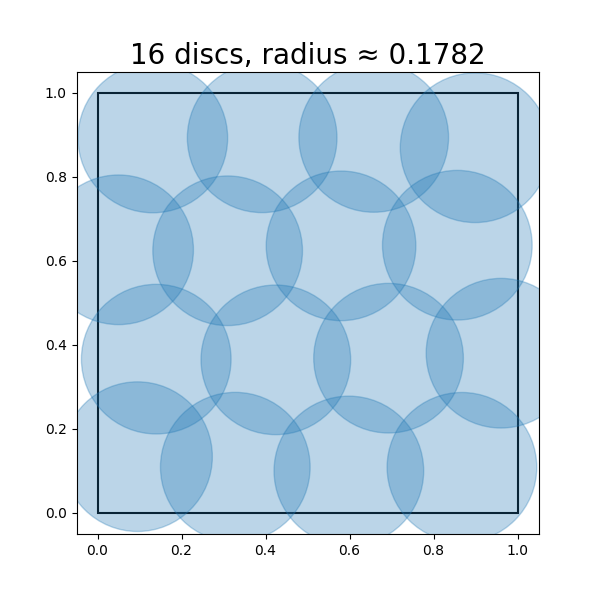
\includegraphics[width=0.3\textwidth]{\toplevelprefix/chapters/chapter3/figs/16.png}
		\hfill
		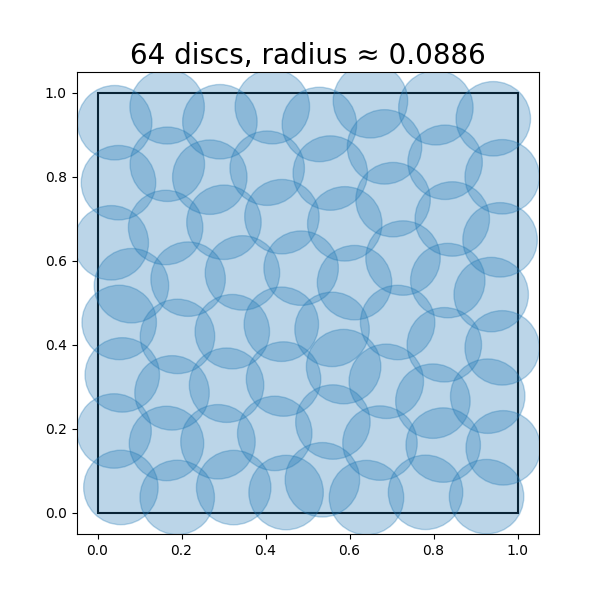
\includegraphics[width=0.3\textwidth]{\toplevelprefix/chapters/chapter3/figs/64.png}
		\hfill
		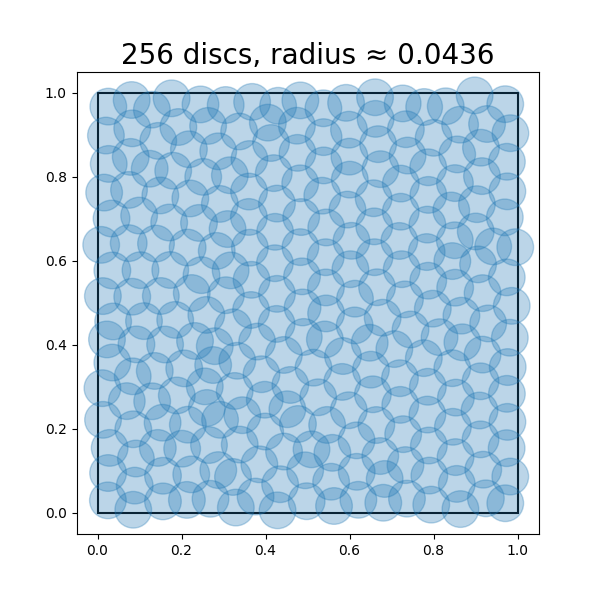
\includegraphics[width=0.3\textwidth]{\toplevelprefix/chapters/chapter3/figs/256.png}

		\caption{Aproximări ale soluțiilor optime pentru \(2^{4}\), \(2^{6}\) și \(2^{8}\) discuri care acoperă un pătrat, împreună cu razele corespunzătoare, calculate folosind un algoritm de optimizare euristică.}
		\label{fig:seven-circles-packing}
	\end{figure}
\end{example}

\begin{figure}[t]
	\centering 
	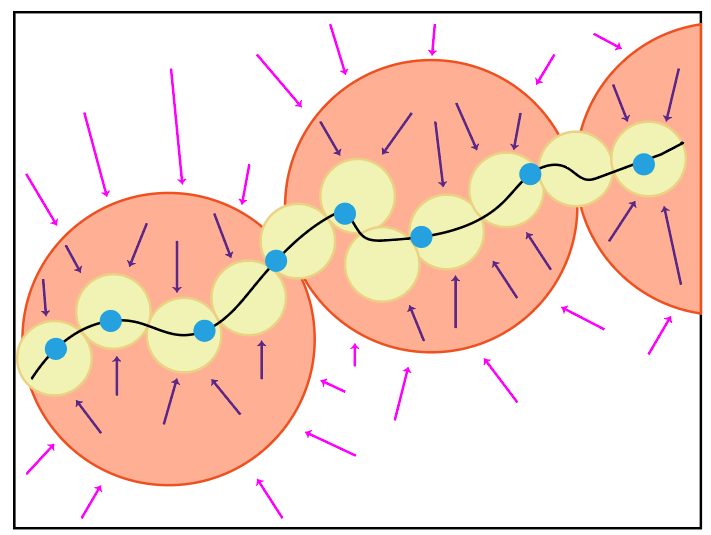
\includegraphics[width=0.6\textwidth]{\toplevelprefix/chapters/chapter3/figs/continuation.png}
	\caption{\small\textbf{Aproximarea unei distribuții cu dimensiuni reduse prin \(\epsilon\)-bile.} Putem vedea că pe măsură ce parametrul \(\epsilon\) se micșorează, uniunea \(\epsilon\)-bilelor aproximează suportul distribuției adevărate (negru) din ce în ce mai bine. Mai mult, denoiser-ii asociați (a căror mapare intrare-ieșire este dată de săgețile furnizate) obținuți prin aproximarea distribuției adevărate printr-un amestec de Gaussiene, fiecare cu covarianță \((\epsilon^{2}/D)\vI\), aproximează din ce în ce mai bine denoiser-ii adevărați. La \(\epsilon\) mare, astfel de denoiseri nu indică deloc spre distribuția adevărată, în timp ce la \(\epsilon\) mic ei aproximează îndeaproape denoiser-ii adevărați. \Cref{thm:covering-number-rate-distortion} stabilește că această aproximare caracterizează funcția ratei distorsiunii la distorsiuni mici $\epsilon$, unificând abordările paralele ale minimizării ratei de codificare și îndepărtării zgomotului pentru învățarea distribuțiilor cu dimensiuni reduse fără patologii.}
	\label{fig:continuation}
\end{figure}

Se dovedește a fi o problemă notoriu de dificilă să obținem expresii în formă închisă pentru funcția ratei distorsiunii \eqref{eqn:rate-distortion-general} pentru distribuții generale $p(\vx)$. Cu toate acestea, așa cum sugerează \Cref{example:sphere-covering-rate-distortion}, există cazuri speciale importante în care \textit{geometria} suportului distribuției $p(\vx)$ poate fi legată de funcția ratei distorsiunii și prin urmare de rata optimă de codificare la nivelul de distorsiune $\epsilon$.
De fapt, acest exemplu poate fi generalizat la orice setare în care suportul lui $p(\x)$ este un set compact suficient de regulat—inclusiv distribuții cu dimensiuni reduse—și $p(\x)$ este distribuit uniform pe suportul său.
Aceasta acoperă un număr vast de cazuri de interes practic.
Formalizăm această noțiune în următorul rezultat, care stabilește această proprietate pentru un caz special.

\begin{theorem}\label{thm:covering-number-rate-distortion}
	Să presupunem că \(\vx\) este o variabilă aleatoare astfel încât suportul său \(K \doteq \Supp(\vx)\) este un set compact. Definim \textit{numărul de acoperire} \(\cN_{\epsilon}(K)\) ca numărul minim de bile de rază \(\epsilon\) care pot acoperi \(K\), i.e.,
	\begin{equation}
		\cN_{\epsilon}(K) \doteq \min\left\{n \in \bN \colon \exists \vp_{1}, \dots, \vp_{n} \in K\ \text{s.t.}\ K \subseteq \bigcup_{i = 1}^{n}B_{\epsilon}(\vp_{i})\right\},
	\end{equation}
	unde \(B_{\epsilon}(\vp) = \set{\vxi\in \R^D \given \norm{\vxi - \vp}_2 \leq \epsilon}\) este bila euclidiană de rază \(\epsilon\) centrată la \(\vp\).
	Atunci avem
	\begin{equation}
		\cR_{\epsilon}(\vx) 
		\leq \log_{2} \cN_{\epsilon}(K).
	\end{equation}
	Dacă, în plus, $\vx$ este distribuit uniform pe $K$ și $K$ este un amestec de subspații ortogonale mutuale de rang redus,\footnote{De fapt, este posibil să tratăm $K$ foarte neregulat, cum ar fi fractalii, cu un rezultat paralel, dar enunțul său devine mult mai tehnic: c.f.\ Riegler et al.\ \cite{Riegler2018-jh,Riegler2023-rr}. Oferim o demonstrație simplă în \Cref{app:rate-distortion-covering} care arată rezultatul pentru amestecuri de subspații.}
	atunci o limită inferioară corespunzătoare este valabilă:
	\begin{equation}
		\cR_{\epsilon}(\vx)
		\geq
		\log_{2} \cN_{\epsilon}(K) - O(D).
	\end{equation}
\end{theorem}
\begin{proof}
O demonstrație a acestei teoreme este dincolo de scopul acestei cărți și o amânăm pentru \Cref{app:rate-distortion-covering}.
\end{proof}

\begin{remark}\label{rem:slb}
	Ingredientul cheie în demonstrația limitei inferioare din
	\Cref{thm:covering-number-rate-distortion} este un rezultat important din
	teoria informației cunoscut sub numele de \textit{limita inferioară Shannon} pentru rata
	distorsiunii, numită după Claude Shannon, care a derivat-o prima dată într-un caz special
	\cite{shannon1959coding}. Aceasta
	afirmă următoarea estimare pentru funcția ratei distorsiunii, pentru orice variabilă
	aleatoare $\x$ cu
	o densitate $p(\x)$ și normă pătrată așteptată finită \cite{Linder1994-ej}:
	\begin{equation}\label{eq:slb}
		\cR_{\epsilon}(\x)
		\geq
		h(\x)
		- \log_2 \volume(B_{\epsilon})
		-
		C_D,
	\end{equation}
	unde $C_D > 0$ este o constantă care depinde doar de $D$. Mai mult, această limită inferioară
	este atinsă cu egalitate pentru distribuții \textit{gaussiene}. Această teoremă nu numai
	că oferă o estimare optimă a cât de mulți biți sunt necesari pentru a codifica o
	distribuție gaussiană, dar oferă și un schema explicită de codificare.
	O schiță a demonstrației este oferită în \Cref{app:rate-distortion-covering}.
\end{remark}

Implicația \Cref{thm:covering-number-rate-distortion} poate fi rezumată după cum urmează: pentru codificarea suficient de precisă a distribuției lui $\x$, cadrul de codificare cu rata minimă a distorsiunii este complet caracterizat de problema împachetării sferelor pe suportul lui $\x$.
Esența demonstrației \Cref{thm:covering-number-rate-distortion} poate fi într-adevăr generalizată la distribuții mai complexe, cum ar fi amestecuri suficient de incoerente de varietăți, dar lăsăm aceasta pentru un studiu viitor.
Deci rata distorsiunii poate fi gândită ca o modalitate „conștientă de probabilitate" de a aproxima suportul distribuției lui \(\vx\) printr-un amestec de multe bile mici.

Acum discutăm o altă conexiune între aceasta și ierarhia de complexitate îndepărtare a zgomotului-difuzie-entropie pe care am discutat-o mai devreme în acest capitol.

\subsection{Rata de Codificare cu Pierderi pentru o Gaussiană cu Dimensiuni Reduse}\label{subsec:lossy DR}
Acum să presupunem că ni se dă un set de eșantioane de date în $\X = [\x_1, \ldots, \x_N]$ din orice distribuție.\footnote{Sau aceste puncte de date ar putea fi văzute ca o distribuție (empirică) ele însele.} Am dori să venim cu o schemă constructivă care poate codifica datele până la o anumită precizie, să zicem
\begin{equation}
	\x_i \mapsto \hat \x_i, \quad \mbox{cu constrângerea} \quad \|\x_i - \hat \x_i\|_2 \le \epsilon.
\end{equation}
Observați că aceasta este o condiție suficientă, explicită și interpretabilă care asigură că datele sunt codificate astfel încât \(\frac{1}{N}\sum_{i = 1}^{N} \norm{\x_i- \hat \x_i}_2^{2} \le \epsilon^{2}\). Această ultimă inegalitate este exact constrângerea ratei distorsiunii pentru distribuția empirică furnizată și codificarea sa. De exemplu, în \Cref{example:sphere-covering-rate-distortion}, am folosit acest criteriu simplificat pentru a găsi explicit distorsiunea minimă și schema de codificare explicită pentru o rată de codificare dată.

Fără pierderea generalității, să presupunem că media lui $\X$ este zero, i.e., $\frac{1}{N} \sum_{i = 1}^{N} \x_i = \boldsymbol{0}$. Fără nicio cunoaștere prealabilă despre natura distribuției din spatele lui $\X$, putem vedea $\X$ ca eșantionat dintr-o distribuție Gaussiană $\mathcal{N}(\boldsymbol{0}, {\boldsymbol{\Sigma}})$ cu covarianța\footnote{Se știe că dată o varianță fixă, Gaussiana atinge entropia maximă. Adică, oferă o limită superioară pentru ce ar putea fi cel mai rău caz în termeni de rată de codificare posibilă.}
\begin{equation}
	{\boldsymbol{\Sigma}} = \frac{1}{N} \X\X^\top.
\end{equation}
Observați că geometric ${\boldsymbol{\Sigma}}$ caracterizează o regiune elipsoidală unde rezidă majoritatea eșantioanelor $\x_i$.

Putem vedea $\hat \X = [\hat \x_1,\ldots, \hat \x_N]$ ca o versiune zgomotoasă a lui $\X = [\x_1, \ldots, \x_N]$:
\begin{equation}
	\hat \x_i = \x_i + \vw_i,
\end{equation}
unde $\vw_i$ este un zgomot Gaussian $\vw_i  \sim \mathcal{N}(\boldsymbol{0} , {\epsilon^2}  \boldsymbol{I}/{D})$ independent de $\vx_i$. Atunci covarianța lui $\hat \x_i$ este dată de
\begin{equation}
	\hat{\boldsymbol{\Sigma}} = \mathbb{E}\left[\hat \x_i \hat \x_i^\top\right] = \frac{\epsilon^2}{D} \boldsymbol{I} + \frac{1}{N} \X\X^\top.
\end{equation}

Observați că volumul regiunii întinse de vectorii $\x_i$ este proporțional cu rădăcina pătrată a determinantului matricei de covarianță
\begin{equation}
	\mbox{volum}(\hat \x_i) \propto \sqrt{\det \big(\hat{\boldsymbol{\Sigma}}\big)} = \sqrt{\det\left(\frac{\epsilon^2}{D} \boldsymbol{I} + \frac{1}{N} \X\X^\top \right)}.
\end{equation}
Volumul întins de fiecare vector aleator $\boldsymbol{w}_i$ este proporțional cu
\begin{equation}
	\mbox{volum}(\boldsymbol{w}_i) \propto   \sqrt{\det\left(\frac{\epsilon^2}{D} \boldsymbol{I} \right)}.
\end{equation}

\begin{figure}
	\centering
	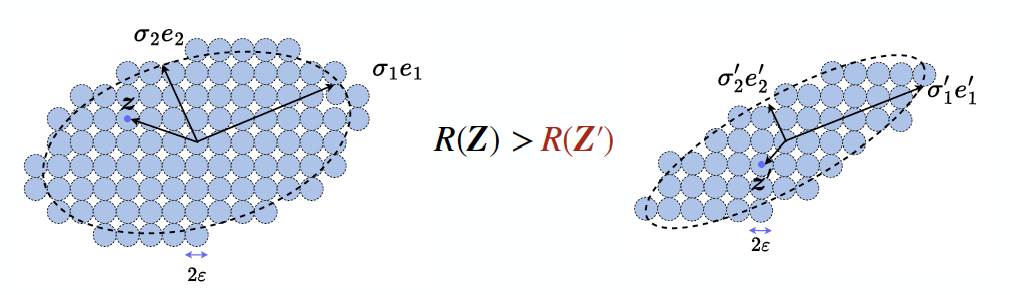
\includegraphics[width=\linewidth]{\toplevelprefix/chapters/chapter3/figs/Gaussian-compression.png}
	\caption{Acoperirea regiunii întinse de vectorii de date folosind $\epsilon$-bile. Cu cât volumul spațiului este mai mare, cu atât sunt necesare mai multe bile, prin urmare sunt necesari mai mulți biți pentru a codifica și enumera bilele. Fiecare vector cu valori reale $\vx$ poate fi codificat ca numărul bilei în care cade.}
	\label{fig:ball-packing}
\end{figure}

Pentru a codifica vectori care cad în regiunea întinsă de $\hat \x_i$, putem acoperi regiunea cu bile ne-suprapuse de rază $\epsilon$, așa cum este ilustrat în \Cref{fig:ball-packing}. Când volumul regiunii întinse de $\hat \x_i$ este semnificativ mai mare decât volumul $\epsilon$-bilei, numărul total de bile de care avem nevoie pentru a acoperi regiunea este aproximativ egal cu raportul celor două volume:
\begin{equation}
	\# \,\epsilon\mbox{-bile} \approx \frac{\mbox{volum}(\hat \vx_i)}{\mbox{volum}(\vw_i)} = \sqrt{\det\left(\boldsymbol{I} + \frac{D}{N\epsilon^2} \X\X^\top  \right)}.
\end{equation}
Dacă folosim numere binare pentru a eticheta toate $\epsilon$-bilele din regiunea de interes, numărul total de biți binari necesari este astfel
\begin{equation} 
	\cR_{\epsilon}(\X) \approx \log_2 (\# \,\epsilon\mbox{-bile}) \approx R_{\epsilon}(\X) \doteq \frac{1}{2} \log \det \left(\boldsymbol{I} + \frac{D}{N\epsilon^2} \X\X^\top \right).
	\label{eqn:rate-Gaussian}
\end{equation}

\begin{example}
	Figura \ref{fig:ball-packing} arată un exemplu al unei distribuții 2D cu un suport elipsoidal -- aproximând suportul unei distribuții Gaussiene 2D. Regiunea este acoperită de bile mici de dimensiune $\epsilon$. Toate bilele sunt numerotate de la $1$ la să zicem $n$. Atunci dat orice vector $\x$ în această regiune, trebuie doar să determinăm cărei $\epsilon$-bile îi este cel mai apropiat, notat ca $\operatorname{ball}_{\epsilon}(\x)$. Pentru a reține $\x$, trebuie doar să reținem numărul acestei bile, care necesită $\log(n)$ biți pentru a stoca. Dacă trebuie să decodificăm $\x$ din acest număr, pur și simplu luăm $\hat \x$ ca centrul bilei. Aceasta duce la o schemă explicită de codificare și decodificare:
	\begin{equation}
		\x \longrightarrow \operatorname{ball}_{\epsilon}(\x) \longrightarrow \hat \x = \mbox{centrul lui} \operatorname{ball}_{\epsilon}(\x).
	\end{equation}
	Se pot referi la aceste centre de bile ca ``coduri'' ale unei cărți de coduri sau dicționar pentru schema de codificare. Este ușor de văzut că precizia acestei scheme de codificare-decodificare (cu pierderi) este aproximativ raza bilei $\epsilon$.
	În mod clar $\cR_{\epsilon}(\Z)$ este numărul mediu de biți necesari pentru a codifica numărul bilei fiecărui vector $\z$ cu această schemă de codificare și prin urmare poate fi numit {\em rata de codificare} asociată cu această schemă.
\end{example}

Din derivarea de mai sus, știm că rata de codificare $\cR_{\epsilon}(\X)$ este (aproximativ) realizabilă cu o schemă explicită de codificare (și decodificare). Are două proprietăți interesante:
\begin{itemize}
	\item În primul rând, se poate observa că $R_{\epsilon}(\X)$ seamănă îndeaproape cu funcția ratei distorsiunii unei surse Gaussiene \cite{Cover-Thomas}. Într-adevăr, când $\epsilon$ este mic, expresia de mai sus este o aproximare apropiată a ratei distorsiunii unei surse Gaussiene, așa cum a fost indicat de \cite{MaY2007-PAMI}.
	\item În al doilea rând, aceeași rată de codificare în formă închisă $R_{\epsilon}(\X)$ poate fi derivată ca o aproximare a \(\cR_{\epsilon}(\vX)\) dacă datele $\X$ sunt presupuse a fi dintr-un subspațiu liniar. Aceasta poate fi arătată prin cuantificarea corectă a descompunerii în valori singulare (SVD) a lui $\X = \boldsymbol{U} \boldsymbol{\Sigma}\boldsymbol{V}^\top$ și construirea unei scheme de codificare cu pierderi pentru vectori în subspațiul întins de $\boldsymbol{U}$ \cite{MaY2007-PAMI}.
\end{itemize}
În contextul nostru, expresia în formă închisă $R_{\epsilon}(\X)$ este destul de fundamentală: este rata de codificare asociată cu o schemă explicită și naturală de codificare cu pierderi pentru date extrase fie dintr-o distribuție Gaussiană sau un subspațiu liniar. După cum vom vedea în următorul capitol, această formulă joacă un rol important în înțelegerea arhitecturii rețelelor neurale profunde.

\subsection{Gruparea unui Amestec de Gaussiene cu Dimensiuni Reduse}
\label{sec:clustering-Gaussians}
După cum am discutat înainte, setul de date dat $\X$ are adesea structuri intrinseci cu dimensiuni reduse. Prin urmare, codificarea sa ca o Gaussiană generală ar fi foarte redundantă. Dacă putem identifica acele structuri intrinseci în $\X$, am putea proiecta scheme de codificare mult mai bune care dau rate de codificare mult mai mici. Sau echivalent, codurile folosite pentru a codifica astfel de $\X$ pot fi comprimate. Vom vedea că compresia oferă o modalitate unificatoare calculabilă de a identifica astfel de structuri. În această secțiune, demonstrăm această idee importantă cu cea mai de bază familie de structuri cu dimensiuni reduse: un amestec de Gaussiene (cu dimensiuni reduse) sau subspații.

\begin{example}
	\Cref{fig:two-subspaces} arată un exemplu în care datele $\X$ sunt distribuite în jurul a două subspații (sau Gaussiene cu dimensiuni reduse). Dacă sunt văzute și codificate împreună ca o singură Gaussiană, cartea de coduri discretă (cu pierderi) asociată, reprezentată de toate bilele albastre, este evident foarte redundantă. Putem încerca să identificăm locațiile celor două subspații, notate cu $S_1$ și $S_2$, și să proiectăm o carte de coduri care acoperă doar cele două subspații, i.e., bilele verzi. Dacă putem partiția corect eșantioanele din datele $\X$ în cele două subspații: $\X = [\X_1, \X_2]\bm \Pi$ cu $\X_1 \in S_1$ și $\X_2 \in S_2$, unde $\bm \Pi$ denotă o matrice de permutare, atunci rata de codificare rezultată pentru date va fi mult mai mică. Aceasta dă o reprezentare mai parcimonioasă, prin urmare mai dezirabilă, a datelor.
\end{example}

\begin{figure}
	\centering
	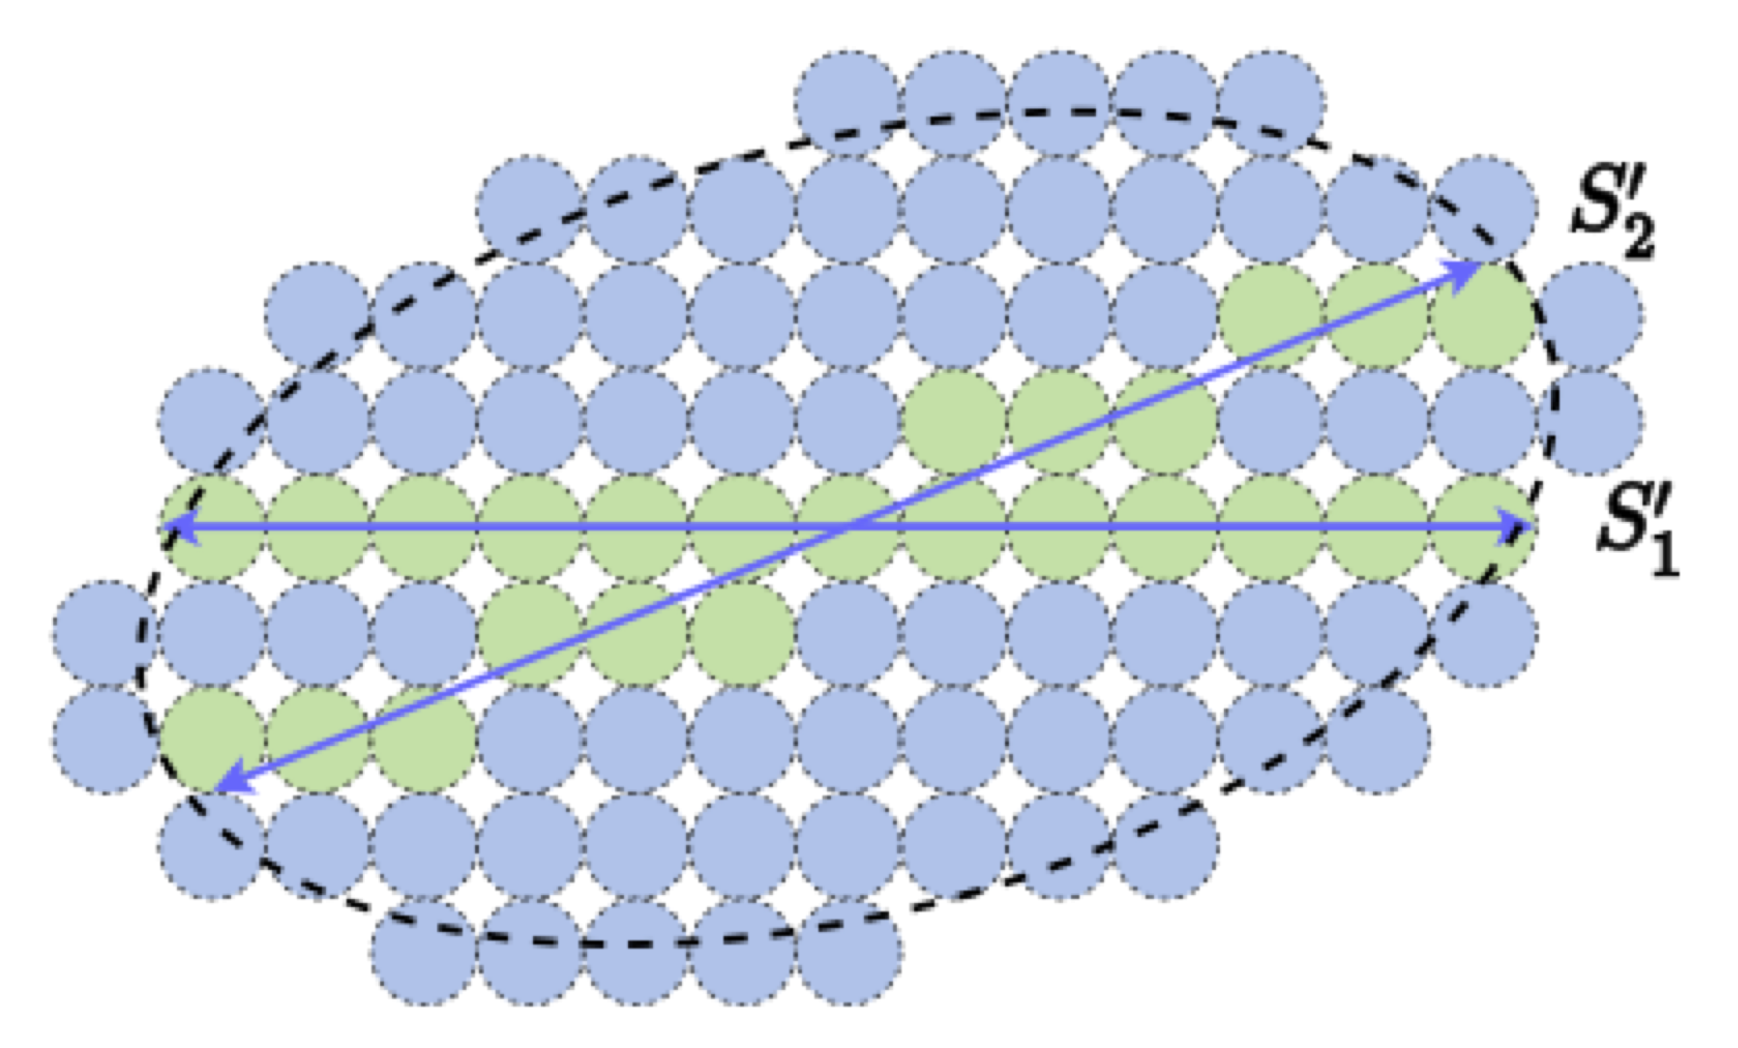
\includegraphics[width=0.5\linewidth]{\toplevelprefix/chapters/chapter3/figs/Two-subspaces.png}
	\caption{Comparație a două scheme de codificare cu pierderi pentru date care sunt distribuite în jurul a două subspații. Una este să împachetăm $\epsilon$-bile (albastre) pentru întregul spațiu întins de cele două subspații; cealaltă este să împachetăm bile doar într-o vecinătate tabulară în jurul celor două subspații. Ultima are în mod evident o carte de coduri mult mai mică și rezultă într-o rată de codificare mult mai mică pentru eșantioane pe subspații.}
	\label{fig:two-subspaces}
\end{figure}

Deci, mai general vorbind, dacă datele sunt extrase din orice amestec de subspații sau Gaussiene cu dimensiuni reduse, ar fi de dorit să identificăm acele componente și să codificăm datele pe baza dimensiunilor intrinseci ale acelor componente. Se dovedește că nu pierdem multă generalitate presupunând că datele sunt extrase dintr-un amestec de Gaussiene cu dimensiuni reduse. Aceasta deoarece un amestec de Gaussiene poate aproxima îndeaproape majoritatea distribuțiilor generale \cite{borkar2016gaussian}.

\paragraph{Problema grupării.}
Acum pentru această familie specifică de distribuții, cum putem identifica efectiv și eficient acele componente cu dimensiuni reduse dintr-un set de eșantioane
\begin{equation}
	\X = \left[\x_1, \x_2, \ldots, \x_N\right],
\end{equation}
extrase din ele? Cu alte cuvinte, dat întregul set de date $\X$, vrem să-l partițăm, sau grupăm, în multiple, să zicem $K$, subseturi:
\begin{equation}
	\X\bm \Pi = [\X_1, \X_2, \dots, \X_K],
\end{equation}
unde fiecare subset constă din eșantioane extrase doar dintr-o Gaussiană cu dimensiuni reduse sau subspațiu și $\bm \Pi$ este o matrice de permutare pentru a indica apartenența partiției. Observați că, în funcție de situație, partiția ar putea fi fie deterministă sau probabilistică. Așa cum s-a arătat în \cite{ma2007segmentation}, pentru amestecul de Gaussiene, partiția probabilistică nu duce la o rată de codificare mai mică. Deci pentru simplitate, considerăm aici doar o partiție deterministă.

\paragraph{Grupare prin compresie cu pierderi.}
Principala dificultate în rezolvarea problemei de grupare de mai sus este că în mod normal nu cunoaștem numărul de clustere $K$, nici nu cunoaștem dimensiunea fiecărei componente. Există o lungă istorie pentru studiul acestei probleme de grupare. Manualul \cite{GPCA} oferă o acoperire sistematică și cuprinzătoare a diferitelor abordări ale acestei probleme. Pentru a găsi o abordare eficientă la această problemă, trebuie mai întâi să înțelegem și să clarificăm de ce vrem să grupăm. Cu alte cuvinte, ce câștigăm exact din gruparea datelor, comparativ cu a nu grupa? Cum măsurăm câștigul? Din perspectiva compresiei datelor, o grupare corectă ar trebui să ducă la o schemă de codificare (și decodificare) mai eficientă.

Pentru orice set de date dat $\X$, există deja două scheme de codificare evidente ca bază de referință. Ele reprezintă două moduri extreme de a codifica datele:
\begin{itemize}
	\item Pur și simplu vedem toate eșantioanele împreună ca extrase dintr-o singură Gaussiană. Rata de codificare asociată este, așa cum a fost derivată înainte, dată de:
	      \begin{equation}
		      \cR_{\epsilon}(\vX) \approx R_{\epsilon}(\X) = \frac{1}{2} \log \det \left(\boldsymbol{I} + \frac{D}{N\epsilon^2} \X\X^\top \right).
	      \end{equation}
	\item Pur și simplu memorăm toate eșantioanele separat prin atribuirea unui număr diferit fiecărui eșantion. Rata de codificare ar fi:
	      \begin{equation}
		      \cR_0(\X) = \log(N).
	      \end{equation}
\end{itemize}

Observați că oricare schemă de codificare poate deveni soluția ``optimă'' pentru o anumită alegere (extremă) a erorii de cuantizare $\epsilon$:
\begin{enumerate}
	\item {\em Regimul Leneș}: Dacă alegem $\epsilon$ să fie extrem de mare, toate eșantioanele din $\X$ pot fi acoperite de o singură bilă. Rata este  $\lim_{\epsilon \rightarrow \infty} \cR_\epsilon \rightarrow \frac{1}{2}\log\det (\boldsymbol{I}) = 0$.
	\item {\em Regimul de Memorare}: Dacă $\epsilon$ este extrem de mic, fiecare eșantion din $\X$  este acoperit de o $\epsilon$-bilă diferită, prin urmare totalul este $N$. Rata este $\lim_{\epsilon \rightarrow 0} \cR_\epsilon \rightarrow \log(N)$.
\end{enumerate}
Observați că prima schemă corespunde scenariului când cineva nu se preocupă deloc de nimic interesant despre distribuție. Nu vrei să economisești niciun bit pentru nimic informativ. Numim aceasta ``regimul leneș''. A doua schemă corespunde scenariului când cineva vrea să decodifice fiecare eșantion cu o precizie extrem de mare. Deci ar fi mai bine să ``memoreze'' fiecare eșantion. Numim aceasta ``regimul de memorare''.
\begin{figure}
	\centering
	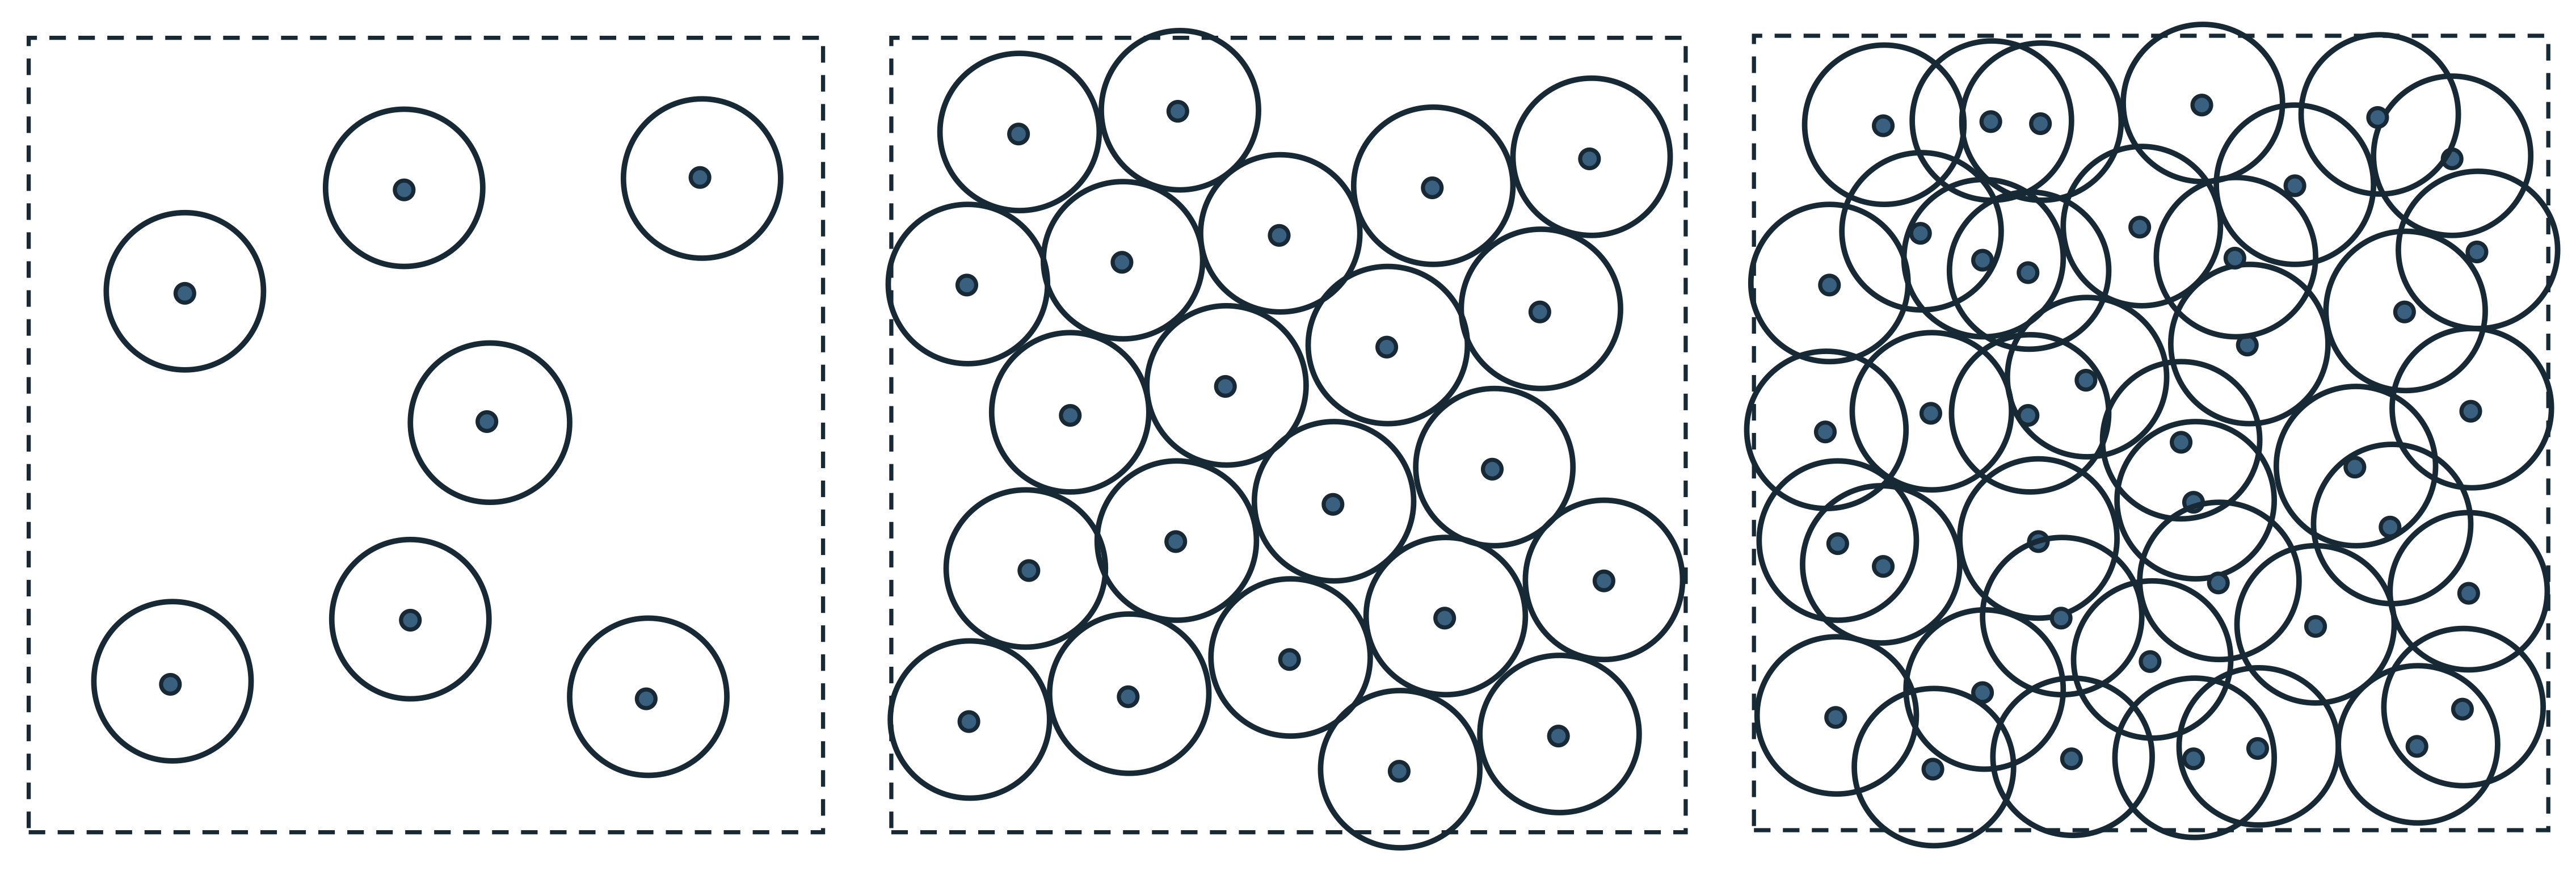
\includegraphics[width=0.9\linewidth]{\toplevelprefix/chapters/chapter3/figs/circle-packing.png}
	\caption{Un număr de eșantioane aleatorii pe un plan 2D. Considerați un $\epsilon$-disc atribuit fiecărui eșantion cu eșantionul ca centru. Densitatea eșantioanelor crește de la stânga la dreapta.}
	\label{fig:circle-packing}
\end{figure}
\begin{example}
	Pentru a vedea când regimul de memorare este preferat sau nu, să considerăm un număr, să zicem $N$, de eșantioane distribuite aleatoriu într-o arie unitară pe un plan 2D.\footnote{Să zicem că punctele sunt extrase printr-un proces Poisson cu densitate $N$ puncte pe unitate de arie.} Imaginați-vă că încercăm să proiectăm o schemă de codificare cu pierderi cu o eroare de cuantizare fixă $\epsilon$. Aceasta este echivalentă cu punerea unui $\epsilon$-disc în jurul fiecărui eșantion, așa cum este arătat în \Cref{fig:circle-packing}. Când $N$ este mic, șansa ca toate discurile să se suprapună între ele este zero. O carte de coduri de dimensiune $N$ este necesară și optimă în acest caz. Când $N$ sau densitatea atinge o anumită valoare critică $N_c$, cu probabilitate mare toate discurile încep să se suprapună și să se conecteze într-un cluster care acoperă întregul plan---acest fenomen este cunoscut ca ``percolație'' continuă \cite{Gilbert-1961,Mertens-Moore-2012}. Când $N$ devine mai mare decât această valoare, discurile se suprapun puternic. Numărul $N$ de discuri devine foarte redundant deoarece vrem doar să codificăm puncte pe plan până la precizia dată $\epsilon$. Numărul de discuri necesare pentru a acoperi toate eșantioanele este mult mai mic decât $N$.\footnote{De fapt, există algoritmi eficienți pentru a găsi o astfel de acoperire \cite{Booth-2001}.}
\end{example}

Atât regimul leneș cât și cel de memorare sunt oarecum triviale și poate sunt de puțin interes teoretic sau practic. Oricare schemă ar fi departe de a fi optimă când este folosită pentru a codifica un număr mare de eșantioane extrase dintr-o distribuție care are un {\em suport compact și cu dimensiuni reduse}. Regimul interesant există între aceste două.
\begin{example}
	\begin{figure}[t]
		\centering
		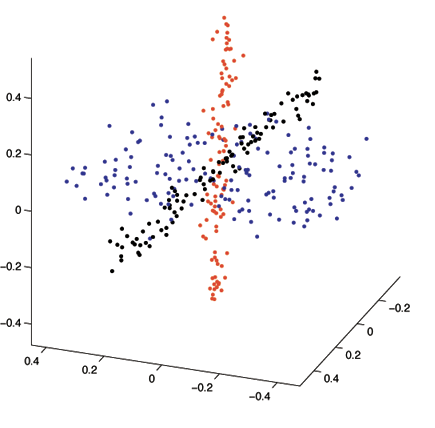
\includegraphics[width=0.4\linewidth]{\toplevelprefix/chapters/chapter3/figs/Two-lines-and-plane.png}
		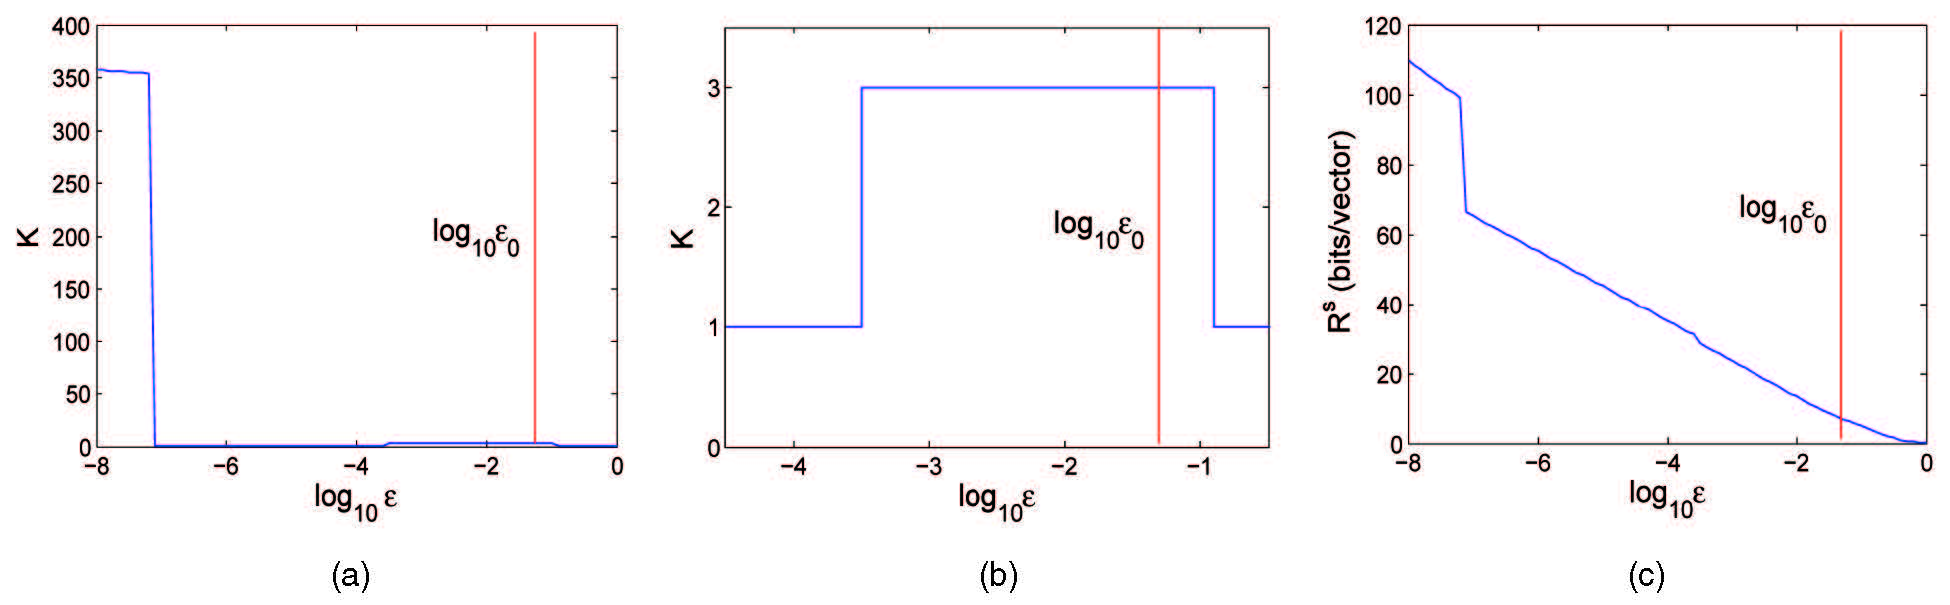
\includegraphics[width=0.9\linewidth]{\toplevelprefix/chapters/chapter3/figs/Coding-Rate.jpg}
		\caption{Sus: 358 eșantioane zgomotoase extrase din două linii și un plan în $\mathbb{R}^3$. Jos: efectul variației lui $\epsilon$ asupra rezultatului grupării și rata de codificare. Linia roșie marchează varianța $\epsilon_0$ a zgomotului Gaussian adăugat la eșantioane.}
		\label{fig:two-lines-and-plane}
		\label{fig:two-lines-and-plane-epsilon}
	\end{figure}
	\Cref{fig:two-lines-and-plane} arată un exemplu cu eșantioane zgomotoase extrase din două linii și un plan în $\mathbb{R}^3$. Așa cum observăm din graficul (c) din dreapta, rata optimă de codificare scade monoton pe măsură ce creștem $\epsilon$, așa cum era anticipat din proprietatea funcției ratei distorsiunii. Graficele (a) și (b) arată, când variază $\epsilon$ de la foarte mic (aproape de zero) la foarte mare (către infinit), numărul optim de clustere când rata de codificare este minimă. Putem vedea clar regimul leneș și regimul de memorare la cele două capete ale graficelor. Dar se poate observa și în graficul (b), când eroarea de cuantizare $\epsilon$ este aleasă să fie în jurul nivelului adevăratei varianțe a zgomotului $\epsilon_0$, numărul optim de clustere este numărul ``corect'' trei care reprezintă două plane și un subspațiu. Ne referim informal la acest regim de mijloc ca ``regimul de generalizare''. Observați că o tranziție de fază ascuțită are loc între aceste regimuri.\footnote{Până acum, din cunoștințele noastre, nu există o justificare teoretică riguroasă pentru aceste comportamente de tranziție de fază.}
\end{example}

Din discuția și exemplele de mai sus, vedem că, atunci când eroarea de cuantizare relativă la densitatea eșantionului\footnote{sau densitatea eșantionului relativă la eroarea de cuantizare} este într-un interval corespunzător, minimizarea ratei de codificare cu pierderi ne-ar permite să descoperim distribuția subiacentă (cu dimensiuni reduse) a datelor eșantionate. {\em Prin urmare, cuantizarea, începută ca o alegere de practicitate, pare să devină necesară pentru învățarea unei distribuții continue din distribuția sa empirică cu eșantioane finite.} Deși o teorie riguroasă pentru explicarea acestui fenomen rămâne evazivă, aici, pentru scopuri de învățare, ne pasă cum să exploatăm fenomenul pentru a proiecta algoritmi care pot găsi distribuția corectă.

Să folosim exemplul simplu arătat în \Cref{fig:two-subspaces} pentru a ilustra ideile de bază. Dacă cineva poate partiția toate eșantioanele din $\X$ în două clustere în $\X_1$ și $\X_2$, cu $N_1$ și $N_2$ eșantioane respectiv, atunci rata de codificare asociată ar fi\footnote{Ignorăm aici câțiva biți suplimentari necesari pentru a codifica apartenența pentru fiecare eșantion, să zicem prin codificarea Huffman.}
\begin{equation}
	R_{\epsilon}^c(\X\mid \boldsymbol{\Pi}) = \frac{N_1}{N}R_{\epsilon}(\X_1) + \frac{N_2}{N}R_{\epsilon}(\X_2),
\end{equation}
unde folosim $\boldsymbol{\Pi}$ pentru a indica apartenența partiției. Dacă partiția respectă structurile cu dimensiuni reduse ale distribuției, în acest caz $\X_1$ și $\X_2$ aparținând celor două subspații respectiv, atunci rata de codificare rezultată ar trebui să fie semnificativ mai mică decât cele două scheme de bază de mai sus:
\begin{equation}
	R_{\epsilon}^c(\X \mid \boldsymbol{\Pi}) \ll R_{\epsilon}(\X), \quad     R_{\epsilon}^c(\X \mid \boldsymbol{\Pi}) \ll R_0(\X).
\end{equation}
În general, putem formula problema de grupare într-o problemă de optimizare care minimizează rata de codificare:
\begin{equation}
	\min_{\boldsymbol{\Pi}}  \bc{ R_{\epsilon}^c(\X \mid \boldsymbol{\Pi})
	\doteq \sum_{k=1}^K \frac{N_k}{N}R_{\epsilon}(\X_k)}.
\end{equation}

\paragraph{Strategii de optimizare pentru grupare.}
Întrebarea rămasă este cum optimizăm obiectivul ratei de codificare de mai sus pentru a găsi clusterele optime. Există trei abordări naturale la acest obiectiv:
\begin{enumerate}
	\item Putem începe cu întregul set $\X$ ca un singur cluster (i.e.\ regimul leneș) și apoi căutăm (să zicem aleatoriu) să-l partițăm astfel încât să ducă la o rată de codificare mai mică.
	\item Invers, putem începe cu fiecare eșantion $\x_i$ ca propriul său cluster (i.e.\ regimul de memorare) și căutăm să îmbinăm clustere care ar rezulta într-o rată de codificare mai mică.
	\item Alternativ, dacă am putea reprezenta (sau aproxima) apartenența $\boldsymbol{\Pi}$ ca niște parametri continui, am putea folosi metode de optimizare precum coborârea gradientului (GD).
\end{enumerate}
Prima abordare nu este atât de atractivă computațional deoarece numărul de partiții posibile pe care trebuie să le încercăm este exponențial în numărul de eșantioane. De exemplu, numărul de partiții ale lui $\X$ în două subseturi de dimensiune egală este $N \choose N/2$ care explodează pe măsură ce $N$ devine mare. Vom explora a treia abordare în următorul \Cref{ch:representation}. Acolo, vom vedea cum rolul rețelelor neurale profunde, în special transformatoarelor, este conectat cu obiectivul ratei de codificare.

Dacă avem două clustere $\X_k$ și $\X_l$, dacă vrem să codificăm eșantioanele ca două clustere separate, lungimea biților binari necesari este
\begin{equation*}
	L^c(\X_k, \X_l) = N_k R_\epsilon(\X_k) + N_l R_\epsilon(\X_l) - N_k \log\frac{N_k}{N_k + N_l} - N_l \log\frac{N_l}{N_k + N_l}.
\end{equation*}
Ultimii doi termeni sunt numărul de biți necesari pentru a codifica apartenența eșantioanelor conform codului Huffman.

Apoi, date fiind oricare două clustere separate $\X_1$ și $\X_2$, putem decide dacă să le îmbinăm sau nu pe baza diferenței dintre cele două lungimi de codificare:
\begin{equation}
	L(\X_k \cup \X_l) - L^c(\X_k, \X_l)
\end{equation}
este pozitivă sau negativă și $\X_k \cup \X_l$ denotă reuniunea seturilor de eșantioane în $\bm X_k$ și $\bm X_l$. Dacă este negativă, înseamnă că lungimea de codificare ar deveni mai mică dacă îmbinăm cele două clustere într-unul singur. Acest fapt simplu duce la următorul algoritm de grupare propus de \cite{ma2007segmentation}:
\begin{algorithm}[!htbp]
	\caption{Descreștere Abruptă pe Perechi a Lungimii de Codificare}\label{alg:steepest_descent_coding_length}
	\begin{algorithmic}[1]
		\Require{\(N\) puncte de date \(\{\vx_{i}\}_{i = 1}^{N}\)}
		\Ensure{Un set \(\cC\) de clustere}

		\Procedure{DescreștereAbruptăPePerechiaLungimiiDeCodificare}{$\{\vx_{i}\}_{i = 1}^{N}$}
		\State{\(\cC \gets \{\{\bm x_{i}\}\}_{i = 1}^{N}\)} \Comment{Inițializează \(N\) clustere \(\vX_{k}\) cu câte un element fiecare}
		\While{\(\abs{\cC} > 1\)}
		\If{\(\displaystyle \min_{\vX_{k}, \vX_{l} \in \cC}[L(\vX_{k} \cup \vX_{l}) -L^{c}(\vX_{k}, \vX_{l})] \geq 0\)} \Comment{Dacă nu se salvează biți prin nicio îmbinare}
		\State{\Return{\(\cC\)}} \Comment{Returnează \(\cC\) și ieși}
		\Else
		\State{\(\displaystyle \vX_{k^{\ast}}, \vX_{l^{\ast}} \gets \argmin_{\vX_{k}, \vX_{l} \in \cC}[L(\vX_{k} \cup \vX_{l}) - L^{c}(\vX_{k}, \vX_{l})]\)} \Comment{Îmbină clusterele care salvează cei mai mulți biți}
		\State{\(\displaystyle \cC \gets [\cC \setminus \{\vX_{k^{\ast}}, \vX_{l^{\ast}}\}] \cup \{\vX_{k^{\ast}} \cup \vX_{l^{\ast}}\}\)} \Comment{Elimină clusterele neîmbinate și adaugă înapoi cel îmbinat}
		\EndIf
		\EndWhile
		\State{\Return{\(\cC\)}}  \Comment{Dacă toate îmbinările produc economii, returnează un cluster}
		\EndProcedure
	\end{algorithmic}
\end{algorithm}

Notați că acest algoritm este tractabil deoarece numărul total de comparații (pe perechi) și îmbinări este de aproximativ $O(N^2\log N)$. Cu toate acestea, datorită naturii sale lacome, nu există nicio garanție teoretică că procesul va converge la soluția de grupare optimă global. Cu toate acestea, după cum s-a raportat în \cite{ma2007segmentation}, în practică, acest algoritm aparent simplu funcționează extrem de bine. Rezultatele de grupare reprezentate în \Cref{fig:two-lines-and-plane} au fost de fapt calculate prin acest algoritm.

\begin{example}[Segmentarea Imaginilor]\label{eg:image-segmentation} Măsura de mai sus a lungimii de codificare și algoritmul de grupare asociat presupun că distribuția datelor este un amestec de Gaussiene (cu dimensiuni reduse). Deși aceasta pare oarecum idealistă, măsura și algoritmul pot fi deja foarte utile și chiar puternice în scenarii când modelul este (aproximativ) valid.

	De exemplu, o imagine naturală constă de obicei din mai multe regiuni cu texturi aproape omogene. Dacă luăm multe ferestre mici din fiecare regiune, ele ar trebui să semene cu eșantioane extrase dintr-o Gaussiană (cu dimensiuni reduse), așa cum este ilustrat în \Cref{fig:image-patch}. \Cref{fig:image-segmentation} arată rezultatele segmentării imaginii pe baza aplicării algoritmului de grupare de mai sus direct pe patch-urile de imagine. Mai multe detalii tehnice privind personalizarea algoritmului la problema segmentării imaginii pot fi găsite în \cite{Mobahi-IJCV2011}.
\end{example}

\begin{figure}
	\centering
	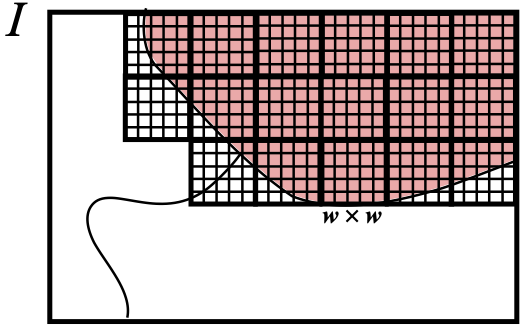
\includegraphics[width=0.4\linewidth]{\toplevelprefix/chapters/chapter3/figs/image-segmentation-tiles.png}
	\caption{Patch-uri de imagine cu o dimensiune de $w\times w$ pixeli.}
	\label{fig:image-patch}
\end{figure}

\begin{figure}[th]
	\centering
	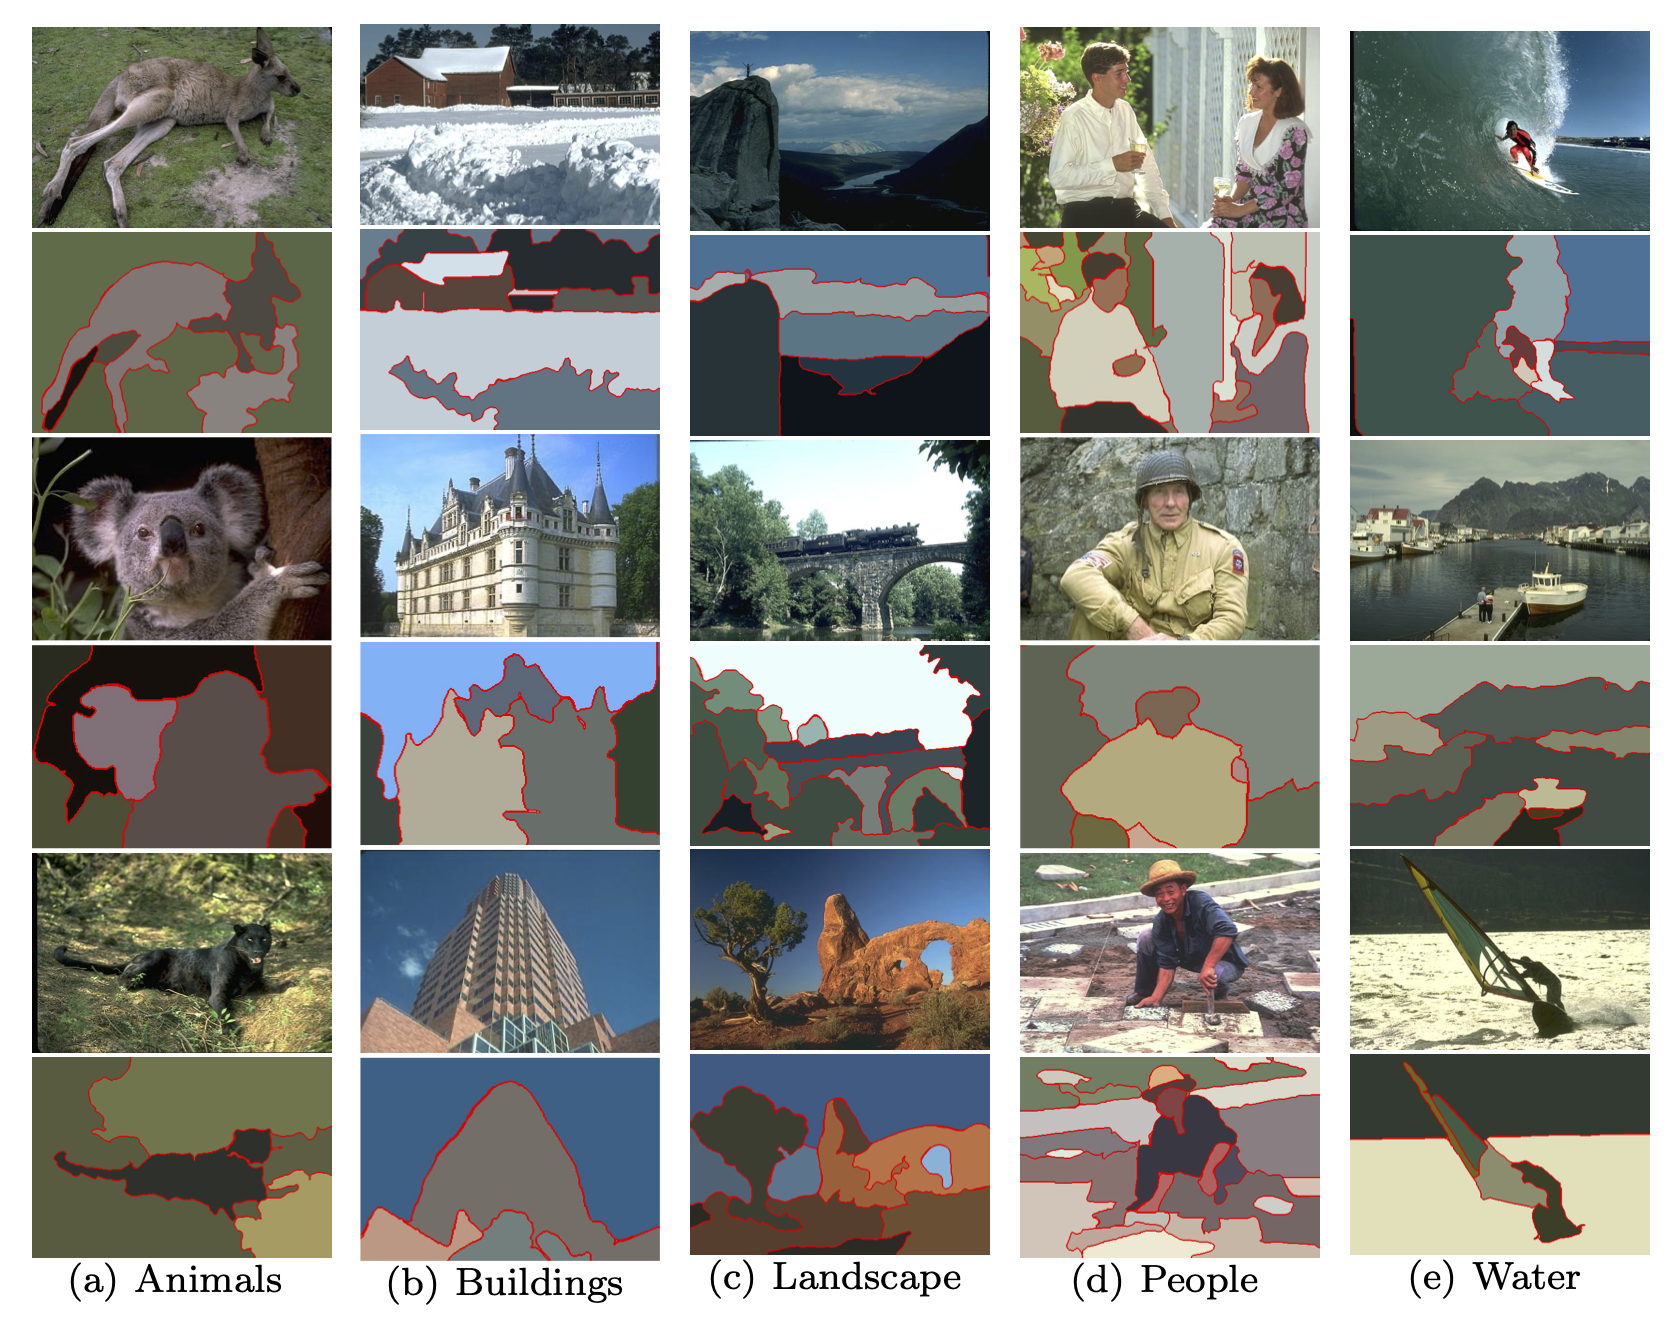
\includegraphics[width=1.0\linewidth]{\toplevelprefix/chapters/chapter3/figs/image-segmentation.png}
	\caption{Segmentarea imaginii bazată pe algoritmul de grupare a ratei de codificare.}
	\label{fig:image-segmentation}
\end{figure}

\section{Maximizarea Câștigului de Informație}
\label{sec:chap4-representation-learning-problem}

Până acum în acest capitol, am discutat cum să identificăm o distribuție cu structuri cu dimensiuni reduse prin principiul compresiei. După cum am văzut din secțiunile anterioare două, compresia computațională poate fi realizată fie prin operația de îndepărtare a zgomotului sau clustering. \Cref{fig:Gaussian-Subspaces} ilustrează acest concept cu exemplul nostru favorit.
\begin{figure}[t]
    \centering
    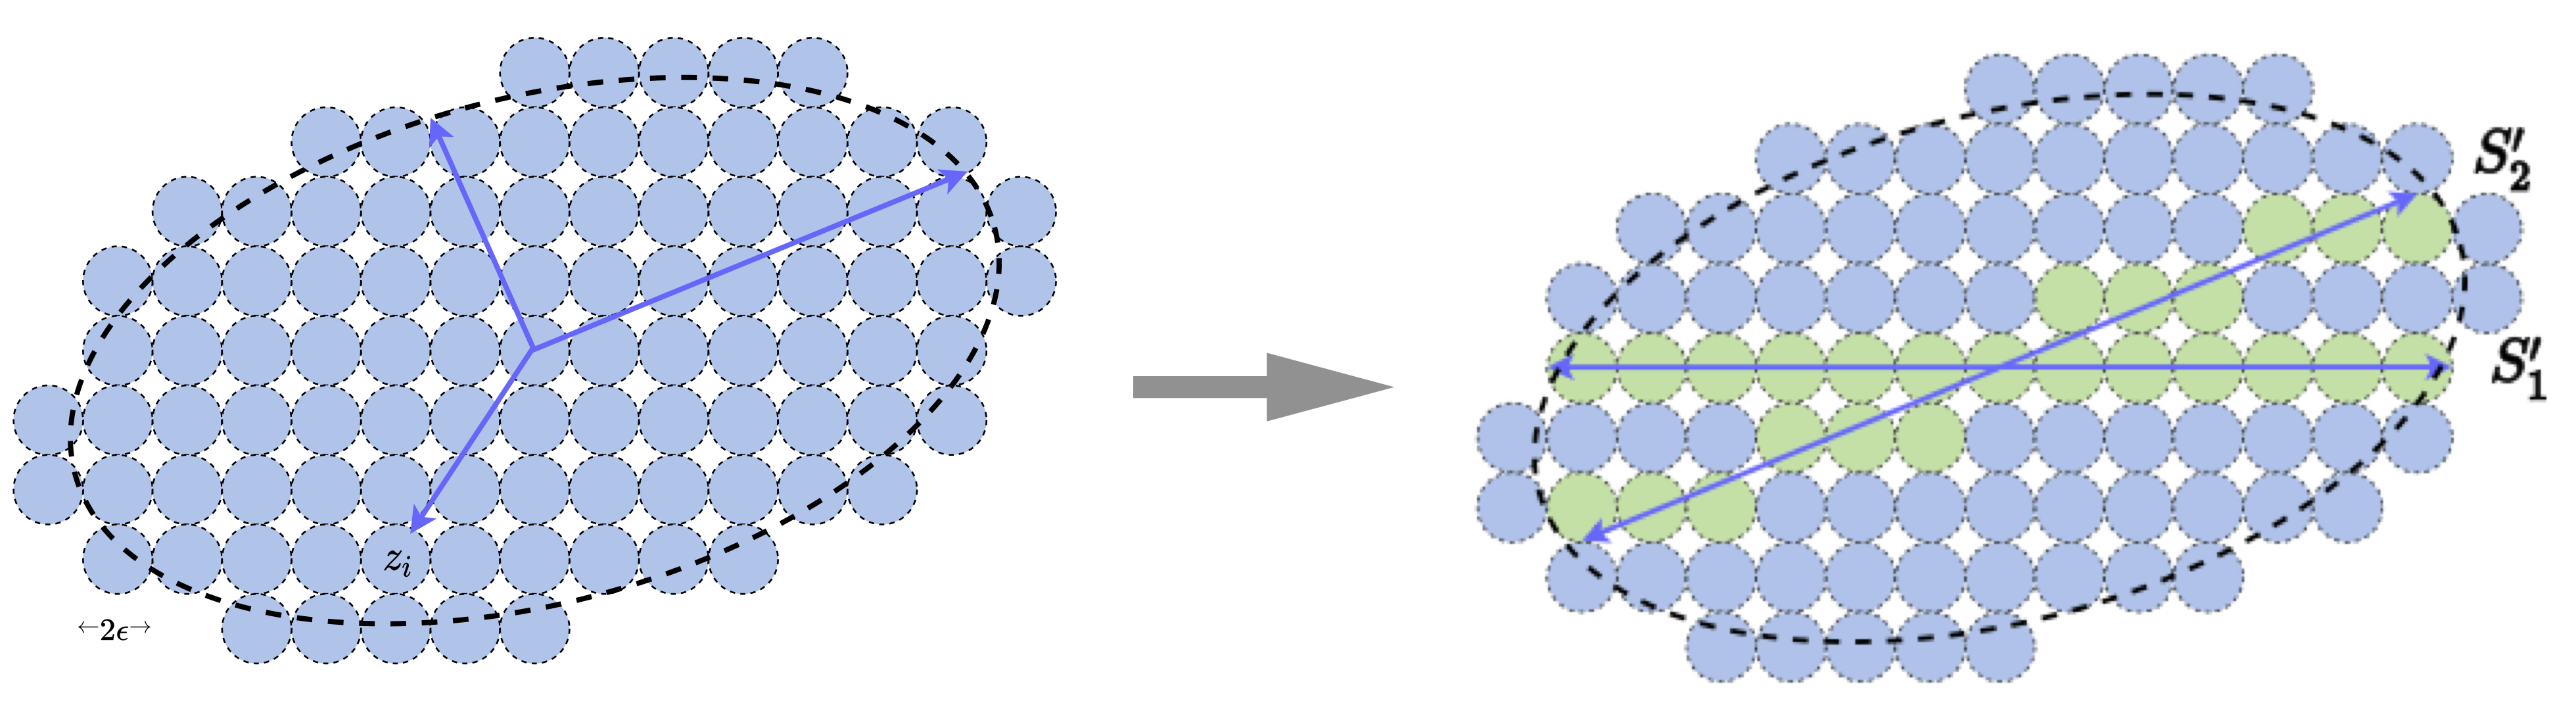
\includegraphics[width=0.8\linewidth]{\toplevelprefix/chapters/chapter3/figs/Gaussian-Subspaces.png}
    \caption{Identificarea unei distribuții cu dimensiuni reduse cu două subspații (stânga) prin îndepărtarea zgomotului sau clustering, pornind de la o distribuție Gaussiană aleatorie generică (dreapta).}
    \label{fig:Gaussian-Subspaces}
\end{figure}
Desigur, scopul final pentru identificarea unei distribuții de date este să o folosim pentru a facilita anumite sarcini ulterioare precum segmentarea, clasificarea sau generarea (de imagini). Prin urmare, modul în care distribuția rezultată este ``reprezentată'' contează enorm cu privire la modul în care informațiile legate de aceste sarcini ulterioare pot fi recuperate și utilizate eficient și efectiv. Aceasta ridică în mod natural o întrebare fundamentală: {\em ce face o reprezentare cu adevărat ``bună'' pentru utilizare ulterioară?} În cele ce urmează, vom explora proprietățile esențiale pe care o reprezentare semnificativă și utilă ar trebui să le posede și cum aceste proprietăți pot fi caracterizate și urmărite explicit prin maximizarea câștigului de informație.

\paragraph{Cum să măsurăm calitatea reprezentărilor.}
Se poate vedea un set de date dat ca eșantioane ale unui vector aleator $\x$ cu o anumită distribuție într-un spațiu cu dimensiuni înalte, să zicem $\mathbb{R}^D$. De obicei, distribuția lui $\x$ are o dimensiune intrinsecă mult mai mică decât spațiul ambiental. În general, {\em învățarea unei reprezentări} se referă la învățarea unei mapări continue, să zicem $f(\cdot)$, care transformă $\x$ într-un așa-numit {\em vector de caracteristici} $\z$ într-un alt spațiu (de obicei cu dimensiuni mai mici), să zicem $\mathbb{R}^d$, unde $d < D$. Se speră că prin o astfel de mapare
\begin{equation}
	\x \in \mathbb{R}^D \xrightarrow{\hspace{2mm} f(\x)\hspace{2mm}} \z  \in \mathbb{R}^d,
	\label{eqn:chap4-1-encoding}
\end{equation}
structurile intrinseci cu dimensiuni reduse ale lui $\x$ sunt identificate și reprezentate de $\z$ într-un mod mai compact și structurat pentru a facilita sarcinile ulterioare precum clasificarea sau generarea. Caracteristica $\z$ poate fi văzută ca un cod (învățat) compact pentru datele originale $\x$, astfel încât maparea $f$ este numită și \textit{codificator}.
Întrebarea fundamentală a învățării reprezentărilor este
\begin{center}
	\noindent{\em Care este o măsură principială și eficientă pentru calitatea reprezentărilor?}
\end{center}

Conceptual, calitatea unei reprezentări $\z$ depinde de cât de bine identifică informația cea mai relevantă și suficientă a lui $\x$ pentru sarcinile ulterioare și cât de eficient reprezintă această informație.
Pentru mult timp, s-a crezut și s-a argumentat că „suficiența" sau „calitatea" unei reprezentări de caracteristici învățate ar trebui să fie definită în termenii unei sarcini specifice. De exemplu, $\z$ trebuie doar să fie suficient pentru a prezice eticheta de clasă $\y$ într-o problemă de clasificare. Mai jos, să începem cu problema clasică a clasificării imaginilor și să argumentăm de ce o astfel de noțiune de „reprezentare" specifică sarcinii este limitată și trebuie să fie generalizată.

\subsection{Reprezentări Discriminative Liniare}\label{subsec:LDR}

Presupunem că $\bm{x} \in \mathbb{R}^D$ este un vector aleator extras dintr-un amestec de $K$ distribuții (componente) $\mathcal{D} = \{\mathcal{D}_k\}_{k=1}^K$. Dat un set finit de eșantioane i.i.d. $\X = [\x_1, \x_2, \ldots, \x_N] \in \Re^{D\times N}$ ale vectorului aleator $\bm x$, {\em căutăm o reprezentare bună} printr-o mapare continuă $f(\x): \mathbb{R}^D \rightarrow \mathbb{R}^d$ care captează structurile intrinseci ale lui $\x$ și facilitează cel mai bine sarcina ulterioară de clasificare.\footnote{Clasificarea este domeniul în care învățarea profundă a demonstrat succesul inițial, declanșând interesul exploziv pentru rețelele profunde. Deși studiul nostru se concentrează pe clasificare, credem că ideile și principiile pot fi generalizate natural la alte setări, cum ar fi regresia.} Pentru a ușura sarcina de învățare a distribuției $\mathcal{D}$, în setarea populară de clasificare supervizată, o etichetă de clasă adevărată (sau un cuvânt cod pentru fiecare clasă), reprezentată de obicei printr-un vector one-hot $\y_i \in \mathbb{R}^K$, este dată pentru fiecare eșantion $\x_i$.

\paragraph{Codificarea informației de clasă prin entropie încrucișată.} Studii extinse au arătat că pentru multe seturi de date practice (de exemplu, imagini, audio și limbaje naturale), maparea (de codificare) de la datele $\bm{x}$ la eticheta sa de clasă $\bm{y}$ poate fi modelată eficient prin antrenarea unei rețele profunde,\footnote{Aici să nu ne îngrijorăm încă despre ce rețea ar trebui să folosim aici și de ce. Scopul aici este să luăm în considerare orice rețea profundă testată empiric. Vom lăsa justificarea arhitecturilor de rețea pentru următorul capitol.} notată aici ca $$f(\x, \theta):\x \mapsto \y$$ cu parametrii rețelei $\theta \in \Theta$, unde $\Theta$ denotă spațiul parametrilor. Pentru ca ieșirea $f(\x, \theta)$ să se potrivească bine cu eticheta $\y$, dorim să minimizăm {\em pierderea de entropie încrucișată} pe un set de antrenare $\{(\x_i, \y_i)\}_{i=1}^N$:
\begin{equation}
   \min_{\theta \in \Theta} \; - \mathbb{E}[\langle \y, \log(f(\x, \theta)) \rangle] \, \approx - \frac{1}{N}\sum_{i=1}^N \langle \y_i, \log\left(f(\x_i, \theta)\right) \rangle.
   \label{chap4-eqn:cross-entropy}
\end{equation}
Parametrii optimi ai rețelei $\theta$ sunt găsiți de obicei prin optimizarea obiectivului de mai sus printr-o schemă eficientă de coborâre a gradientului, cu gradienții calculați prin propagare înapoi (BP), așa cum este descris în \Cref{app:BP-section} din \Cref{app:optimization}.

În ciuda eficacității și popularității sale enorme, există două limitări serioase cu această abordare: 1) Își propune doar să prezică etichetele $\y$ chiar dacă ar putea fi etichetate greșit. Studiile empirice arată că rețelele profunde, folosite ca o „cutie neagră", pot chiar să se potrivească cu etichete aleatoare~\cite{zhang2017understanding}.
2) Cu o astfel de potrivire a datelor de la capăt la capăt, în ciuda multor eforturi empirice în încercarea de a interpreta caracteristicile învățate astfel, nu este clar în ce măsură caracteristicile intermediare învățate de rețea captează structurile intrinseci ale datelor care fac posibilă clasificarea semnificativă în primul rând. Proprietățile geometrice și statistice precise ale caracteristicilor învățate sunt de asemenea adesea obscure, ceea ce duce la lipsa de interpretabilitate și garanții de performanță ulterioare (de exemplu, generalizabilitate, transferabilitate și robustețe etc.) în învățarea profundă.
Prin urmare, {\em unul dintre obiectivele acestei secțiuni este să abordeze astfel de limitări prin reformularea obiectivului către învățarea de reprezentări explicite semnificative și utile pentru datele $\x$, nu limitate la clasificare.}

\begin{figure}
	\centering
	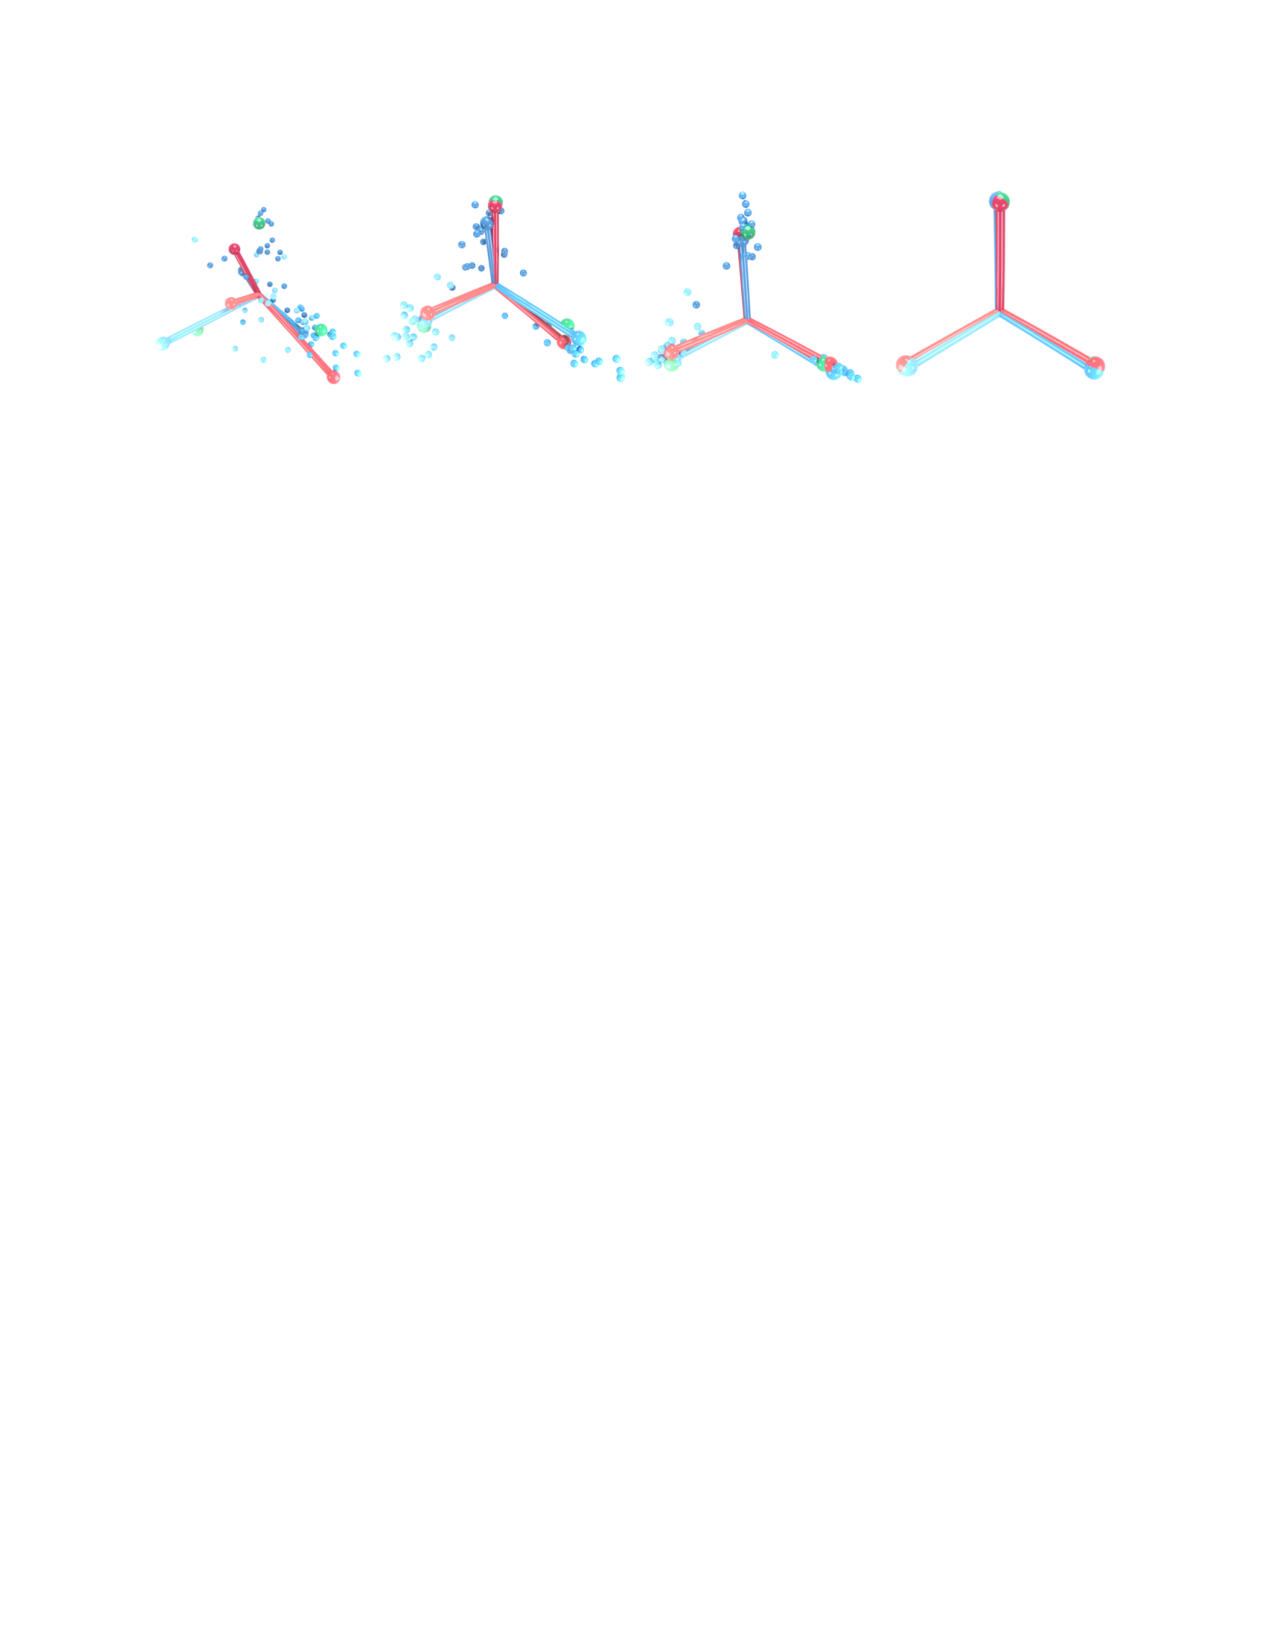
\includegraphics[width=0.95\linewidth]{\toplevelprefix/chapters/chapter3/figs/neural_collapse.pdf}
	\caption{Evoluția ieșirilor stratului penultim ale unei rețele neuronale VGG13 când este antrenată pe setul de date CIFAR10 cu 3 clase selectate aleatoriu. Figura din \cite{papyan2020prevalence}.}
	\label{chap4-fig:neural-collapse}
\end{figure}

\paragraph{Caracteristici discriminative minime prin gâtuire informațională.}
O abordare populară pentru a interpreta rolul rețelelor profunde este de a vedea ieșirile straturilor intermediare ale rețelei ca selectând anumite caracteristici latente $\z = f(\x, \theta) \in \Re^d$ ale datelor care sunt discriminative între mai multe clase. Reprezentările învățate $\z$ facilitează apoi sarcina ulterioară de clasificare pentru prezicerea etichetei de clasă $\y$ prin optimizarea unui clasificator $g(\z)$:
\begin{equation}
	\x   \xrightarrow{\hspace{2mm} f(\x, \theta)\hspace{2mm}} \z  \xrightarrow{\hspace{2mm} g(\z) \hspace{2mm}} \y.
\end{equation}
Știm din teoria informației~\cite{Cover-Thomas} că {\em informația mutuală} între două variabile aleatoare, să zicem $\x,\z$, este definită ca fiind
\begin{equation}
	I(\x; \z) = H(\x) - H(\x\mid \z),
\end{equation}
unde $H(\x \vert \z)$ este entropia condiționată a lui $\x$ dat $\z$. Informația mutuală este cunoscută și ca {\em câștigul de informație}: Măsoară cu cât poate fi redusă entropia variabilei aleatoare $\x$ odată ce $\z$ este dat. Sau echivalent, măsoară câtă informație conține $\z$ despre $\x$. Formularea {\em gâtuirii informaționale} (IB) \cite{Tishby-ITW2015} presupune în plus că rolul rețelei este să învețe $\z$ ca statistica minimă suficientă pentru prezicerea lui $\y$. Formal, caută să maximizeze informația mutuală $I(\z, \y)$ între $\z$ și $\y$ în timp ce minimizează informația mutuală $I(\x, \z)$ între $\x$ și $\z$:
\begin{equation}
	\max_{\theta\in \Theta}\; \mbox{IB}(\x, \y, \z) \doteq I(\z; \y) - \beta I(\x; \z) \quad\ \mathrm{s.t.}\ \z = f(\x, \theta),
	\label{chap4-eqn:information-bottleneck}
\end{equation}
unde $\beta >0$.

Având în vedere că se pot depăși unele avertismente asociate cu acest cadru \cite{kolchinsky2018caveats-ICLR2018}, cum ar fi modul de a evalua cu precizie informația mutuală cu eșantioane finite de distribuții degenerate, acest cadru poate fi util în explicarea anumitor comportamente ale rețelelor profunde.
De exemplu, lucrările recente \cite{papyan2020prevalence} arată într-adevăr că reprezentările învățate prin pierderea de entropie încrucișată \eqref{chap4-eqn:cross-entropy} prezintă un fenomen de \emph{colaps neural}.
Adică, caracteristicile fiecărei clase sunt mapate la un vector unidimensional, în timp ce toate celelalte informații ale clasei sunt suprimate, așa cum este ilustrat în \Cref{chap4-fig:neural-collapse}.
\begin{remark}
    Colapsul neural se referă la un fenomen observat în rețelele neuronale profunde antrenate pentru clasificare, unde reprezentările de caracteristici învățate și ponderile clasificatorului prezintă un comportament extrem de simetric și structurat în timpul fazei terminale de antrenare \cite{papyan2020prevalence,zhu2021geometric}. În mod specific, în cadrul fiecărei clase, caracteristicile colapsează la media lor de clasă, iar între clase, aceste medii devin maxim separate, formând o configurație echiangulară simplă. Clasificatorul liniar se aliniază cu media clasei până la rescalare. În plus, clasificatorul de ultim strat converge pentru a alege orice clasă are cea mai apropiată medie de clasă de antrenare. Colapsul neural dezvăluie conexiuni profunde între dinamica optimizării, generalizarea și structurile geometrice care apar în învățarea supervizată.
\end{remark}

Din exemplul de mai sus al clasificării, vedem că reprezentarea învățată astfel oferă un codificator foarte simplu care în esență mapează fiecare clasă de date la un singur cuvânt cod: vectorul one-hot reprezentând fiecare clasă. Din perspectiva compresiei cu pierderi, un astfel de codificator are prea multe pierderi pentru a păstra informații în distribuția datelor. Alte informații, cum ar fi cele utile pentru sarcini precum generarea de imagini, sunt pierdute sever într-un astfel de proces de învățare supervizată. Pentru a remedia această situație, dorim să învățăm o schemă de codificare diferită astfel încât reprezentarea de caracteristici rezultată să poată captura informații mult mai bogate despre distribuția datelor, nu limitate doar la cele utile pentru clasificare.

\begin{figure}[ht]
	\centering
	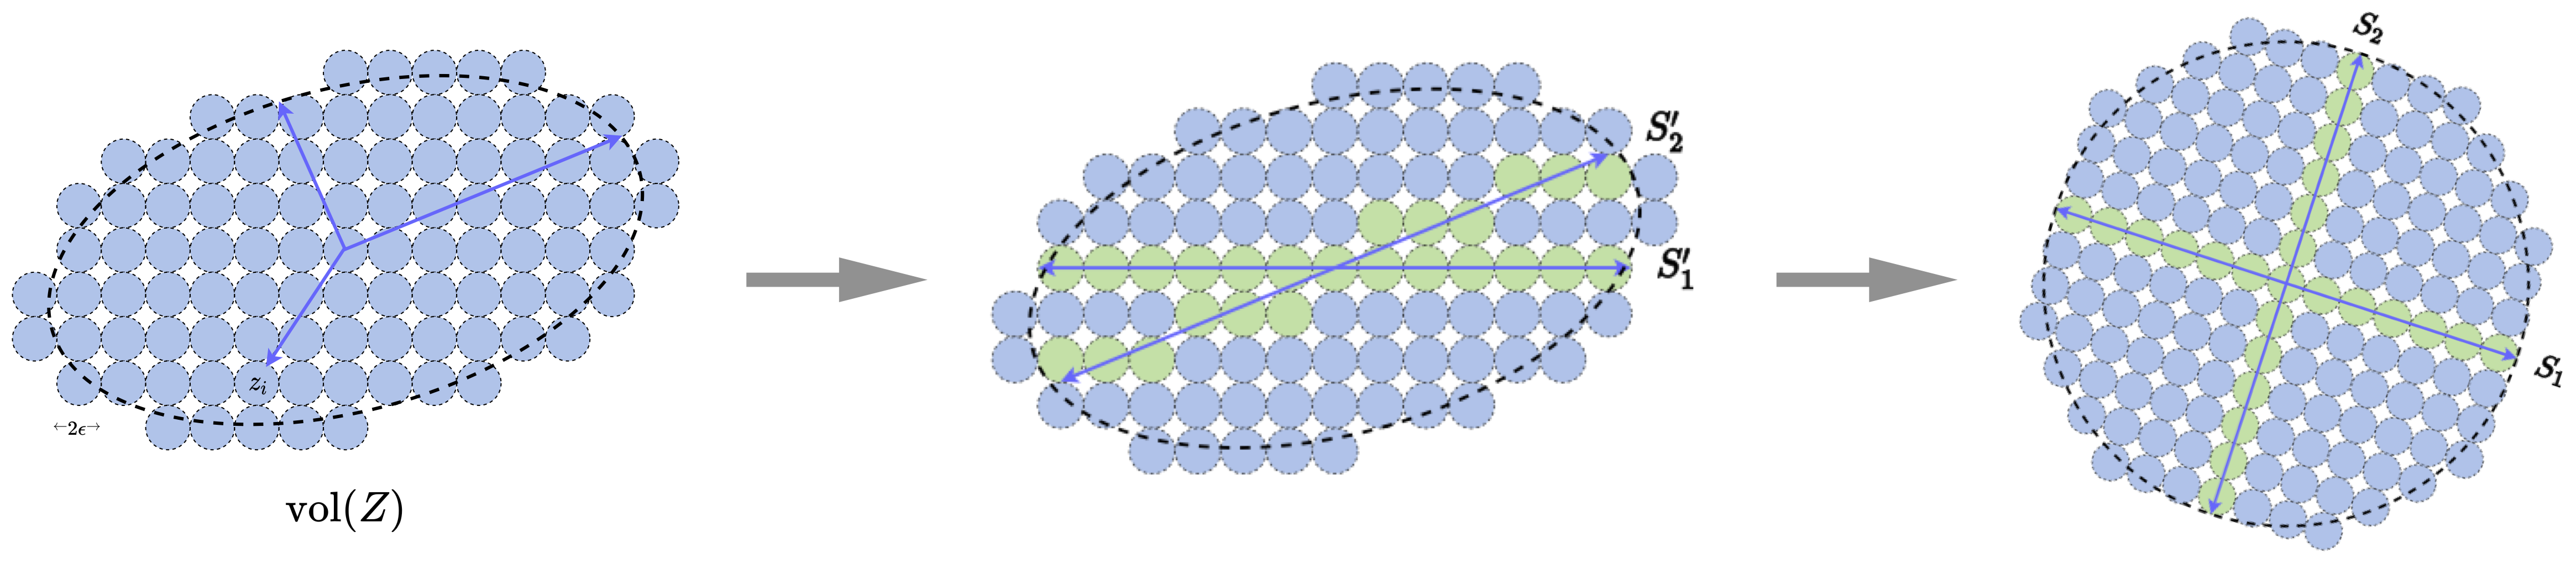
\includegraphics[width=0.99\linewidth]{\toplevelprefix/chapters/chapter3/figs/Expansion2.png}
	\caption{După identificarea distribuției de date cu dimensiuni reduse, am dori să transformăm în continuare distribuția datelor într-o reprezentare cu structură mai informativă: $R$ este numărul de bile de $\epsilon$ care acoperă întregul spațiu și $R^c$ este suma numerelor pentru toate subspațiile (bilele verzi). $\Delta R$ este diferența lor (numărul de bile albastre).}\label{fig:sphere-packing}
	\label{fig:informative-representation}
\end{figure}

\paragraph{Reprezentări discriminative liniare.}
Dacă datele date $\X$ ale unei distribuții mixte $\mathcal{D}$ pot fi clasificate sau grupate efectiv depinde de cât de separabile (sau discriminative) sunt (sau pot fi făcute) distribuțiile componente $\mathcal{D}_k$. O ipoteză de lucru populară este că distribuția fiecărei clase are structuri intrinseci relativ {\em cu dimensiuni reduse}. Prin urmare, putem presupune că distribuția $\mathcal{D}_k$ a fiecărei clase are un suport pe o subvarietate cu dimensiuni reduse, să zicem $\mathcal{M}_k$ cu dimensiunea $d_k \ll D$, iar distribuția $\mathcal D$ a lui $\x$ este suportată pe amestecul acelor subvarietăți, $\mathcal M = \cup_{k=1}^K \mathcal{M}_k$, în spațiul ambiental cu dimensiuni înalte $\Re^D$.

Nu numai că trebuie să identificăm distribuția cu dimensiuni reduse, dar vrem și să reprezentăm distribuția într-o formă care facilitează cel mai bine sarcinile ulterioare precum clasificarea, gruparea și generarea condiționată (cum vom vedea în viitor). Pentru a face acest lucru, cerem ca reprezentările noastre de caracteristici învățate să aibă următoarele proprietăți:
\begin{enumerate}
	\item {\em Compresibile în cadrul clasei:} Caracteristicile eșantioanelor din aceeași clasă ar trebui să fie puternic {\em corelate} în sensul că aparțin unui subspațiu liniar cu dimensiuni reduse.
	\item {\em Discriminative între clase:} Caracteristicile eșantioanelor din clase diferite ar trebui să fie foarte {\em necorelate} și să aparțină unor subspații liniare cu dimensiuni reduse diferite.
	\item {\em Reprezentare maxim diversă:} Dimensiunea (sau varianța) caracteristicilor fiecărei clase ar trebui să fie {\em cât mai mare posibil} atât timp cât sunt incoerente cu celelalte clase.
\end{enumerate}
Ne referim la o astfel de reprezentare ca {\em reprezentare discriminativă liniară} (LDR). Observați că prima proprietate se aliniază bine cu obiectivul clasicei {\em analize a componentelor principale} (PCA) pe care am discutat-o în \Cref{sub:pca}. A doua proprietate seamănă cu cea a clasicei {\em analize discriminante liniare} (LDA)~\cite{HastieTiFr09}. Figura \ref{fig:informative-representation} ilustrează aceste proprietăți cu un exemplu simplu când distribuția datelor este de fapt un amestec de două subspații. Prin compresie (denoising sau grupare), identificăm mai întâi că distribuția adevărată a datelor este un amestec de două subspații cu dimensiuni reduse (mijloc) în loc de o distribuție gaussiană generică (stânga). Apoi am dori să transformăm distribuția astfel încât cele două subspații să devină în cele din urmă mutual incoerente/independente (dreapta).

\begin{remark}
    Analiza discriminantă liniară (LDA)~\cite{HastieTiFr09} este o tehnică de reducere a dimensionalității supervizată care își propune să găsească o proiecție liniară a datelor care maximizează separabilitatea claselor. În mod specific, date fiind date etichetate, LDA caută o transformare liniară care proiectează intrările cu dimensiuni înalte pe un spațiu cu dimensiuni mai mici unde clasele sunt maxim separate. Rețineți că PCA este o metodă nesupervizată care proiectează datele pe direcțiile de varianță maximă fără a lua în considerare etichetele de clasă. În timp ce PCA se concentrează pur pe păstrarea structurii de varianță globală, LDA exploatează explicit informațiile etichetei pentru a îmbunătăți puterea discriminativă; vezi comparația din \Cref{fig:LDA}.
\end{remark}

\begin{figure}
	\centering
	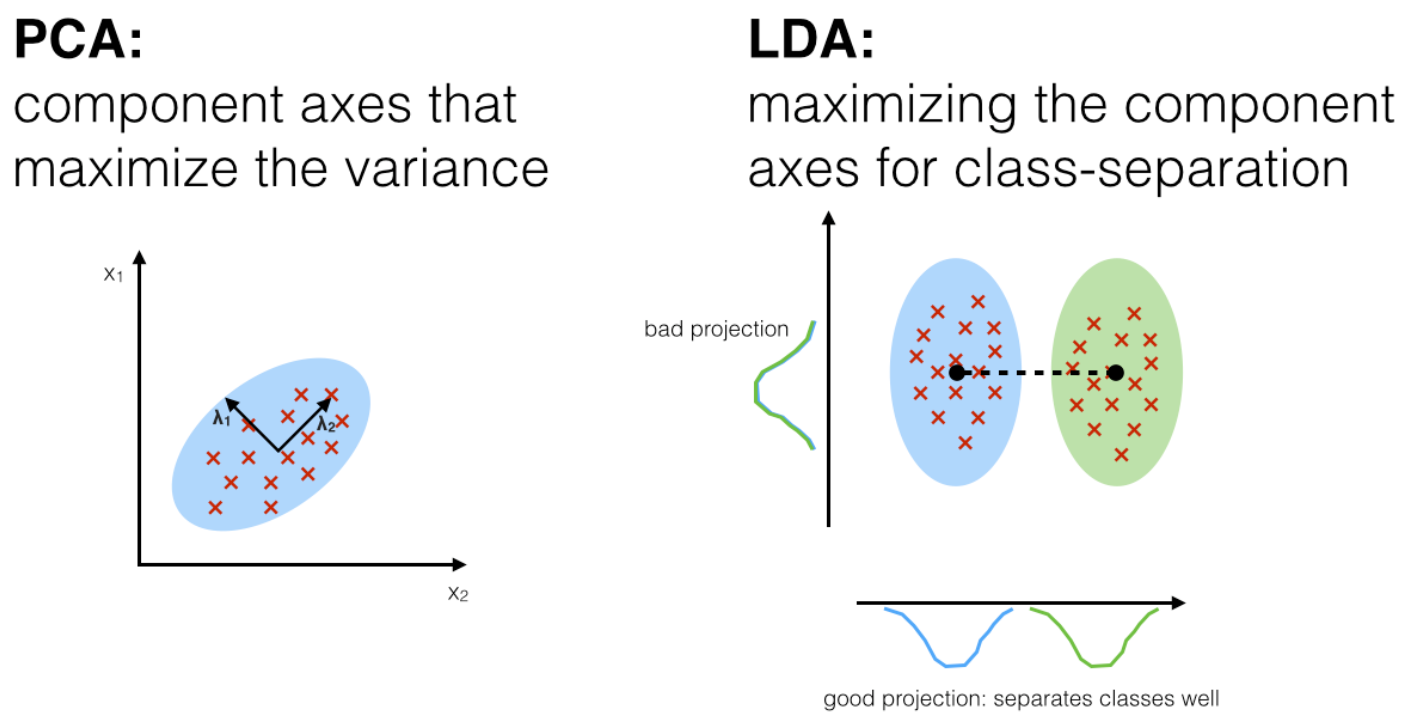
\includegraphics[width=0.7\linewidth]{\toplevelprefix/chapters/chapter3/figs/LDA.png}\vspace{-0.1in}
	\caption{Comparație între PCA și LDA. Figuri adoptate de la \url{https://sebastianraschka.com/Articles/2014_python_lda.html}.}
	\label{fig:LDA}
\end{figure}

A treia proprietate este de asemenea importantă deoarece dorim ca caracteristicile învățate să dezvăluie toate cauzele posibile pentru care o clasă este diferită de toate celelalte clase. De exemplu, pentru a distinge „măr" de „portocală", ne pasă nu doar de culoare, ci și de formă și frunze. În mod ideal, dimensiunea fiecărui subspațiu $\{\mathcal{S}_k\}$ ar trebui să fie egală cu cea a subvarietății corespunzătoare $\mathcal{M}_k$. Această proprietate va fi importantă dacă am dori ca harta $f(\x,\theta)$ să fie {\em inversabilă} pentru sarcini precum generarea de imagini. De exemplu, dacă extragem diferite puncte de eșantion din subspațiul de caracteristici pentru „măr", ar trebui să putem să le decodificăm pentru a genera imagini diverse de mere. Caracteristica învățată din minimizarea entropiei încrucișate \eqref{chap4-eqn:cross-entropy} clar nu are această proprietate.

În general, deși structurile intrinseci ale fiecărei clase/cluster pot fi cu dimensiuni reduse, ele nu sunt în niciun caz pur și simplu liniare (sau gaussiene) în reprezentarea lor originală $\x$ și trebuie să fie făcute liniare mai întâi, printr-o transformare neliniară.\footnote{Vom discuta cum se poate face acest lucru explicit în \Cref{ch:autoencoding}.} Prin urmare, în general, folosim transformarea neliniară $f(\x,\theta)$ pentru a căuta o reprezentare a datelor astfel încât subspațiile care reprezintă toate clasele să fie subspații liniare maxim incoerente. Pentru a fi mai preciși, vrem să învățăm o mapare {$\z = f(\x,\theta)$} care mapează fiecare dintre subvarietățile $\mathcal{M}_k \subset \Re^D$ (\Cref{chap4-fig:mcr-diagram} stânga) la un subspațiu {\em liniar} $\mathcal{S}_k \subset \Re^d$ (\Cref{chap4-fig:mcr-diagram} dreapta). Într-o anumită măsură, subspațiile multiple rezultate $\{\mathcal{S}_k\}$ pot fi văzute ca {\em componente principale generalizate} discriminative \cite{GPCA} sau, dacă sunt ortogonale, {\em componente independente} \cite{hyvarinen2000independent} ale caracteristicilor rezultate $\z$ pentru datele originale $\bm x$.
După cum vom vedea în următorul \Cref{ch:representation}, rețelele profunde joacă exact rolul de modelare și realizare a acestei transformări neliniare de la distribuția datelor la reprezentări discriminative liniare.

\subsection{Principiul Reducerii Maxime a Ratei de Codare}\label{subsec:MCR2}

Deși cele trei proprietăți---{\em discriminative între clase}, {\em compresibile în cadrul clasei} și {\em reprezentare maxim diversă}---pentru reprezentările discriminative liniare (LDR) sunt toate proprietăți foarte dorite ale reprezentării învățate $\z$, ele nu sunt în niciun caz ușor de obținut: Sunt aceste proprietăți compatibile astfel încât să ne putem aștepta să le obținem pe toate odată? Dacă da, există un obiectiv {\em simplu dar principial} care poate măsura calitatea reprezentărilor rezultate în termenii tuturor acestor proprietăți? Cheia acestor întrebări {este să găsim} o „măsură principială de compactitate" sau „câștig de informație" pentru distribuția unei variabile aleatoare $\z$ sau din eșantioanele sale finite $\{\bm z_i\}_{i=1}^N$. O astfel de măsură ar trebui să caracterizeze direct și precis proprietățile geometrice sau statistice intrinseci ale distribuției, în termenii dimensiunii sau {volumului} său intrinsec. Spre deosebire de entropia încrucișată \eqref{chap4-eqn:cross-entropy} sau gâtuirea informațională \eqref{chap4-eqn:information-bottleneck}, o astfel de măsură nu ar trebui să depindă exclusiv de etichetele de clasă, astfel încât să poată funcționa în setări mai generale precum setări supervizate, auto-supervizate, semi-supervizate și nesupervizate.

\begin{figure}
	\centering
	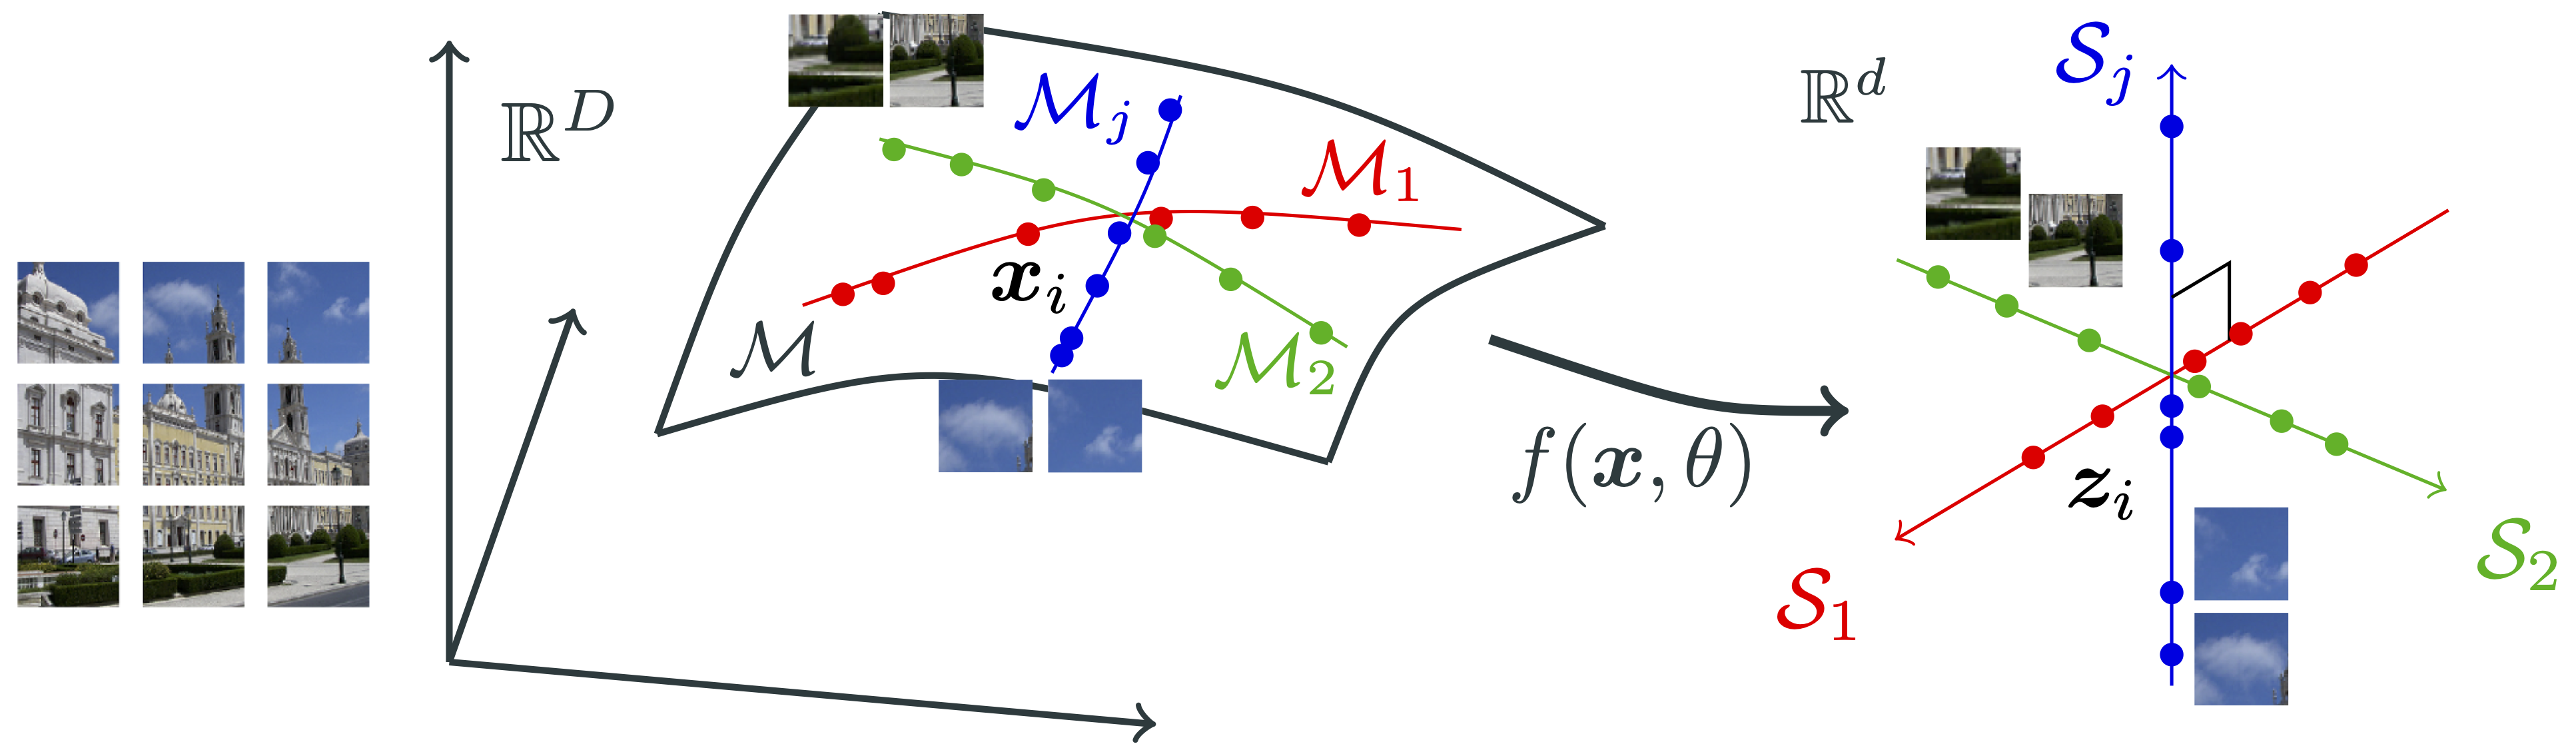
\includegraphics[width=0.8\linewidth]{\toplevelprefix/chapters/chapter3/figs/mcr_diagram.png}
	\caption{Distribuția $\mathcal D$ a datelor cu dimensiuni înalte $\x\in \Re^D$ este suportată pe o varietate $\mathcal{M}$ și clasele sale pe subvarietăți cu dimensiuni reduse $\mathcal{M}_k$. Ne propunem să învățăm o mapare $f(\x, \theta)$ parametrizată de $\theta$ astfel încât $\z_i = f(\x_i, \theta)$ să se afle pe o uniune de subspații maxim necorelatși $\{\mathcal{S}_k\}$.}
	\label{chap4-fig:mcr-diagram}
\end{figure}

Fără pierdere de generalitate, presupunem că distribuția $\mathcal D$ a vectorului aleator $\x$ este suportată pe un amestec de distribuții, adică $\mathcal D = \cup_{k=1}^K \mathcal{D}_k$, unde fiecare $\mathcal{D}_k \subset \Re^D$ are o dimensiune intrinsecă scăzută în spațiul ambiental cu dimensiuni înalte $\Re^D$. Fie $\bm X_k \in \Re^{D\times N_k}$ matricea de date ale cărei coloane sunt eșantioane extrase din distribuția $\mathcal{D}_k$, unde $N_k$ denotă numărul de eșantioane pentru fiecare $k=1,\dots,K$. Apoi, folosim $\bm X=[\bm X_1,\dots,\bm X_K] \in \Re^{D\times N}$ pentru a denota toate eșantioanele, unde $N=\sum_{k=1}^K N_k$.
Amintim că folosim și $\vx_i$ pentru a denota al $i$-lea eșantion al lui $\X$, adică $\X=[\vx_1,\dots,\vx_N]$. Sub o mapare de codificare:
\begin{equation}
	\x   \xrightarrow{\hspace{2mm} f(\x)\hspace{2mm}} \z,
\end{equation}
eșantioanele de intrare sunt mapate la $\vz_i = f(\vx_i)$ pentru fiecare $i=1,\dots,N$. Cu un abuz de notație, scriem și $\Z_k = f(\X_k)$ și $\Z = f(\X)$. Prin urmare, avem $\Z = [\bm Z_1,\dots,\bm Z_K]$ și $\Z = [\vz_1,\dots\vz_N]$.

Pe de o parte, pentru ca caracteristicile învățate să fie discriminative, caracteristicile diferitelor clase/clustere sunt preferate să fie {\em maxim incoerente} între ele. Prin urmare, împreună ar trebui să acopere un spațiu cu cel mai mare volum posibil (sau dimensiune) și rata de codare a întregului set $\Z$ ar trebui să fie cât mai mare posibil. Pe de altă parte, caracteristicile învățate ale aceleiași clase/cluster ar trebui să fie foarte corelate și coerente. Prin urmare, fiecare clasă/cluster ar trebui să acopere doar un spațiu (sau subspațiu) cu un volum foarte mic și rata de codare ar trebui să fie cât mai mică posibil. Acum, vom introduce cum să măsurăm rata de codare a caracteristicilor învățate.

\paragraph{Rata de codare a caracteristicilor.} În mod notabil, o provocare practică în evaluarea ratei de codare este că distribuția de bază a reprezentărilor de caracteristici $\Z$ este de obicei necunoscută. Pentru a aborda acest lucru, putem aproxima caracteristicile $\Z = [\z_1, \ldots, \z_N]$ ca eșantioane extrase dintr-o distribuție gaussiană multivariată. Sub această ipoteză, așa cum s-a discutat în \Cref{subsec:lossy DR}, compactitatea caracteristicilor $\Z$ {\em ca întreg} poate fi măsurată în termenii lungimii medii de codare pe eșantion, denumită {\em rata de codare}, supusă unui nivel de precizie $\epsilon > 0$ (vezi \eqref{eqn:rate-Gaussian}) definită după cum urmează:
\begin{equation}
	R_{\epsilon}(\Z) = \frac{1}{2}\log\det\left(\I + \frac{d}{N\epsilon^{2}}\Z\Z^{\top}\right).
	\label{chap4-eqn:coding-length-eval}
\end{equation}

Pe de altă parte, sperăm că o transformare neliniară $f(\x)$ mapează fiecare subvarietate specifică clasei $\mathcal{M}_k \subset \mathbb{R}^D$ la un subspațiu liniar maxim incoerent $\mathcal{S}_k \subset \mathbb{R}^d$ astfel încât caracteristicile învățate $\Z$ să se afle într-o uniune de subspații cu dimensiuni reduse. Această structură permite o evaluare mai precisă a ratei de codare prin analizarea fiecărui subspațiu separat.
Amintim că coloanele lui $\Z_k$ denotă caracteristicile eșantioanelor din $\X_k$ pentru fiecare $k=1,\dots,K$. Rata de codare pentru caracteristicile din $\bm Z_k$ poate fi calculată după cum urmează:
\begin{align}
    R_{\epsilon}(\Z_k) = \frac{N_k}{2N}\log\det\left(\I + \frac{d}{N_k\epsilon^{2}}\Z_k\Z_k^{\top}\right)
\end{align}
Apoi, suma ratelor medii de codare ale caracteristicilor din fiecare clasă este
\begin{equation}
	 R_{\epsilon}^c(\Z) \doteq \sum_{k=1}^K R_{\epsilon}(\Z_k),
	\label{chap4-eqn:compress-loss-eval}
\end{equation}

Prin urmare, o reprezentare bună $\Z$ a lui $\X$ este cea care realizează o diferență mare între rata de codare pentru întreg și cea pentru toate clasele:
\begin{equation}
	\Delta R_{\epsilon}(\Z) \doteq R_{\epsilon}(\Z) - R_{\epsilon}^c(\Z).
	\label{chap4-eqn:coding-length-reduction}
\end{equation}
Observați că, conform discuțiilor noastre anterioare din acest capitol, această diferență poate fi interpretată ca cantitatea de „informație câștigată" prin identificarea clusterelor corecte cu dimensiuni reduse $\Z_k$ în cadrul setului general $\Z$.

Dacă alegem maparea noastră de caracteristici $f(\cdot)$ să fie o rețea neuronală profundă $f(\cdot,\theta)$ cu parametrii rețelei $\theta$, procesul general al reprezentării caracteristicilor și reducerea ratei rezultată pot fi ilustrate prin următoarea diagramă:
\begin{equation}
	\X
	\xrightarrow{\hspace{2mm} f(\x, \theta)\hspace{2mm}} \Z  \xrightarrow{\hspace{2mm} \epsilon \hspace{2mm}} \Delta R_{\epsilon}(\Z).
	\label{chap4-eqn:flow}
\end{equation}
Rețineți că $\Delta R_{\epsilon}$ este {\em monotonă} în scala caracteristicilor $\Z$. Pentru a asigura o comparație corectă între diferite reprezentări, este esențial să {\em normalizăm scala} caracteristicilor învățate. Aceasta poate fi realizată fie prin impunerea normei Frobenius a fiecărei clase $\Z_k$ să scaleze cu numărul de caracteristici din $\Z_k \in \mathbb R^{d \times N_k}$, adică $\|\Z_k\|_F^2 = N_k$, sau prin normalizarea fiecărei caracteristici să fie pe sfera unitară, adică $\z_i \in \mathbb{S}^{d-1}$, unde $N_k=\mathrm{tr}(\bm \Pi_k)$ denotă numărul de eșantioane din clasa $k$. Această formulare oferă o justificare naturală pentru necesitatea „normalizării pe loturi" în practica antrenării rețelelor neuronale profunde \cite{ioffe2015batch}.

Odată ce reprezentările sunt comparabile, obiectivul devine să învățăm un set de caracteristici $\Z = f(\X, \theta)$ astfel încât să maximizeze reducerea între rata de codare a tuturor caracteristicilor și cea a sumei caracteristicilor în raport cu clasele lor:
\begin{equation}
	\begin{aligned}
		\max_{\theta } & \;  \Delta R_{\epsilon}\big(\Z \big) \doteq R_{\epsilon}(\Z) - R_{\epsilon}^c(\Z ), \\
		\mbox{s.c.} & \ \ \, \Z = f(\bm X, \theta),\  \|\Z_k\|_F^2 = N_k,\ k=1,\dots,K. 
	\end{aligned}
	\label{eqn:maximal-rate-reduction}
\end{equation}
Ne referim la aceasta ca principiul {\em reducerii maxime a ratei de codare} (MCR$^2$), o întruchipare adevărată a celebrului citat al lui Aristotel:
\begin{quote}
	\centering
	„{\em Întregul este mai mare decât suma părților sale.}"
\end{quote}
Pentru a învăța cea mai bună reprezentare, cerem ca {\em întregul să fie maxim mai mare decât suma părților sale}. Să examinăm din nou exemplul arătat în \Cref{fig:informative-representation}. Din perspectiva compresiei, reprezentarea din dreapta este {\em cea mai compactă} în sensul că diferența dintre rata de codare când toate caracteristicile sunt codificate ca o singură gaussiană (albastru) și cea când caracteristicile sunt grupate corespunzător și codificate ca două subspații separate (verde) este maximă.\footnote{Intuitiv, raportul dintre „volumul" întregului spațiu acoperit de toate caracteristicile și cel efectiv ocupat de caracteristici este maxim.}

Rețineți că principiul MCR$^2$ de mai sus este proiectat pentru probleme de învățare supervizată, unde apartenența la grup (sau etichetele de clasă) sunt cunoscute. Cu toate acestea, acest principiu poate fi extins natural la probleme de învățare nesupervizată prin introducerea unei matrici de apartenență, care codifică atribuirea (potențial slabă) a fiecărui punct de date la grupuri sau clustere latente. În mod specific, fie $\bm \Pi = \{\bm \Pi_k\}_{k=1}^K \subset \R^{N\times N}$ un set de matrici diagonale ale căror intrări diagonale codifică apartenența celor $N$ eșantioane în $K$ clase. Adică, $\bm \Pi$ se află într-un simplex $\Omega \doteq \{\bm \Pi: \bm \Pi_k \ge \bm 0: \sum_{k=1}^K \bm \Pi_k = \bm I_N\}$. Apoi, putem defini rata medie de codare în raport cu partiția $\bm \Pi$ ca
\begin{align}\label{eq:MCRc}
    R_{\epsilon}^c(\Z \mid \bm \Pi) \doteq \sum_{k=1}^K \frac{\mathrm{tr}(\bm \Pi_k)}{2N}\log\det\left(\bm I + \frac{d}{\mathrm{tr}(\bm \Pi_k)\epsilon^2}\bm Z\bm \Pi_k \bm Z^\top \right).
\end{align}
Când $\bm Z$ este dat, $R_{\epsilon}^c(\Z \vert \bm \Pi)$ este o funcție concavă a lui $\bm \Pi$. Atunci principiul MCR$^2$ pentru probleme de învățare nesupervizată devine următorul:
\begin{align}\label{eq:MCR-pi}
    \max_{\bm \Pi, \theta} & \  \Delta R_{\epsilon}\big(\Z  \mid \bm \Pi) \doteq R_{\epsilon}(\bm Z) - R_{\epsilon}^c(\Z \mid \bm \Pi) \notag \\ 
   \mathrm{s.c.}  & \ \ \ \bm Z = f(\bm X, \theta),\ \|\bm Z \bm \Pi_k\|_F^2 = N_k,\ k = 1,\dots,K,\ \bm\Pi \in \Omega.

\end{align}
Comparativ cu \eqref{eqn:maximal-rate-reduction}, formularea de aici permite optimizarea comună atât a apartenenței la grup, cât și a parametrilor rețelei. În special, când $\bm \Pi$ este fixat la o matrice de apartenență la grup care atribuie $N$ puncte de date în $K$ grupuri, această problemă poate recupera Problema \eqref{eqn:maximal-rate-reduction}.

\begin{figure}[t]
	\centering
	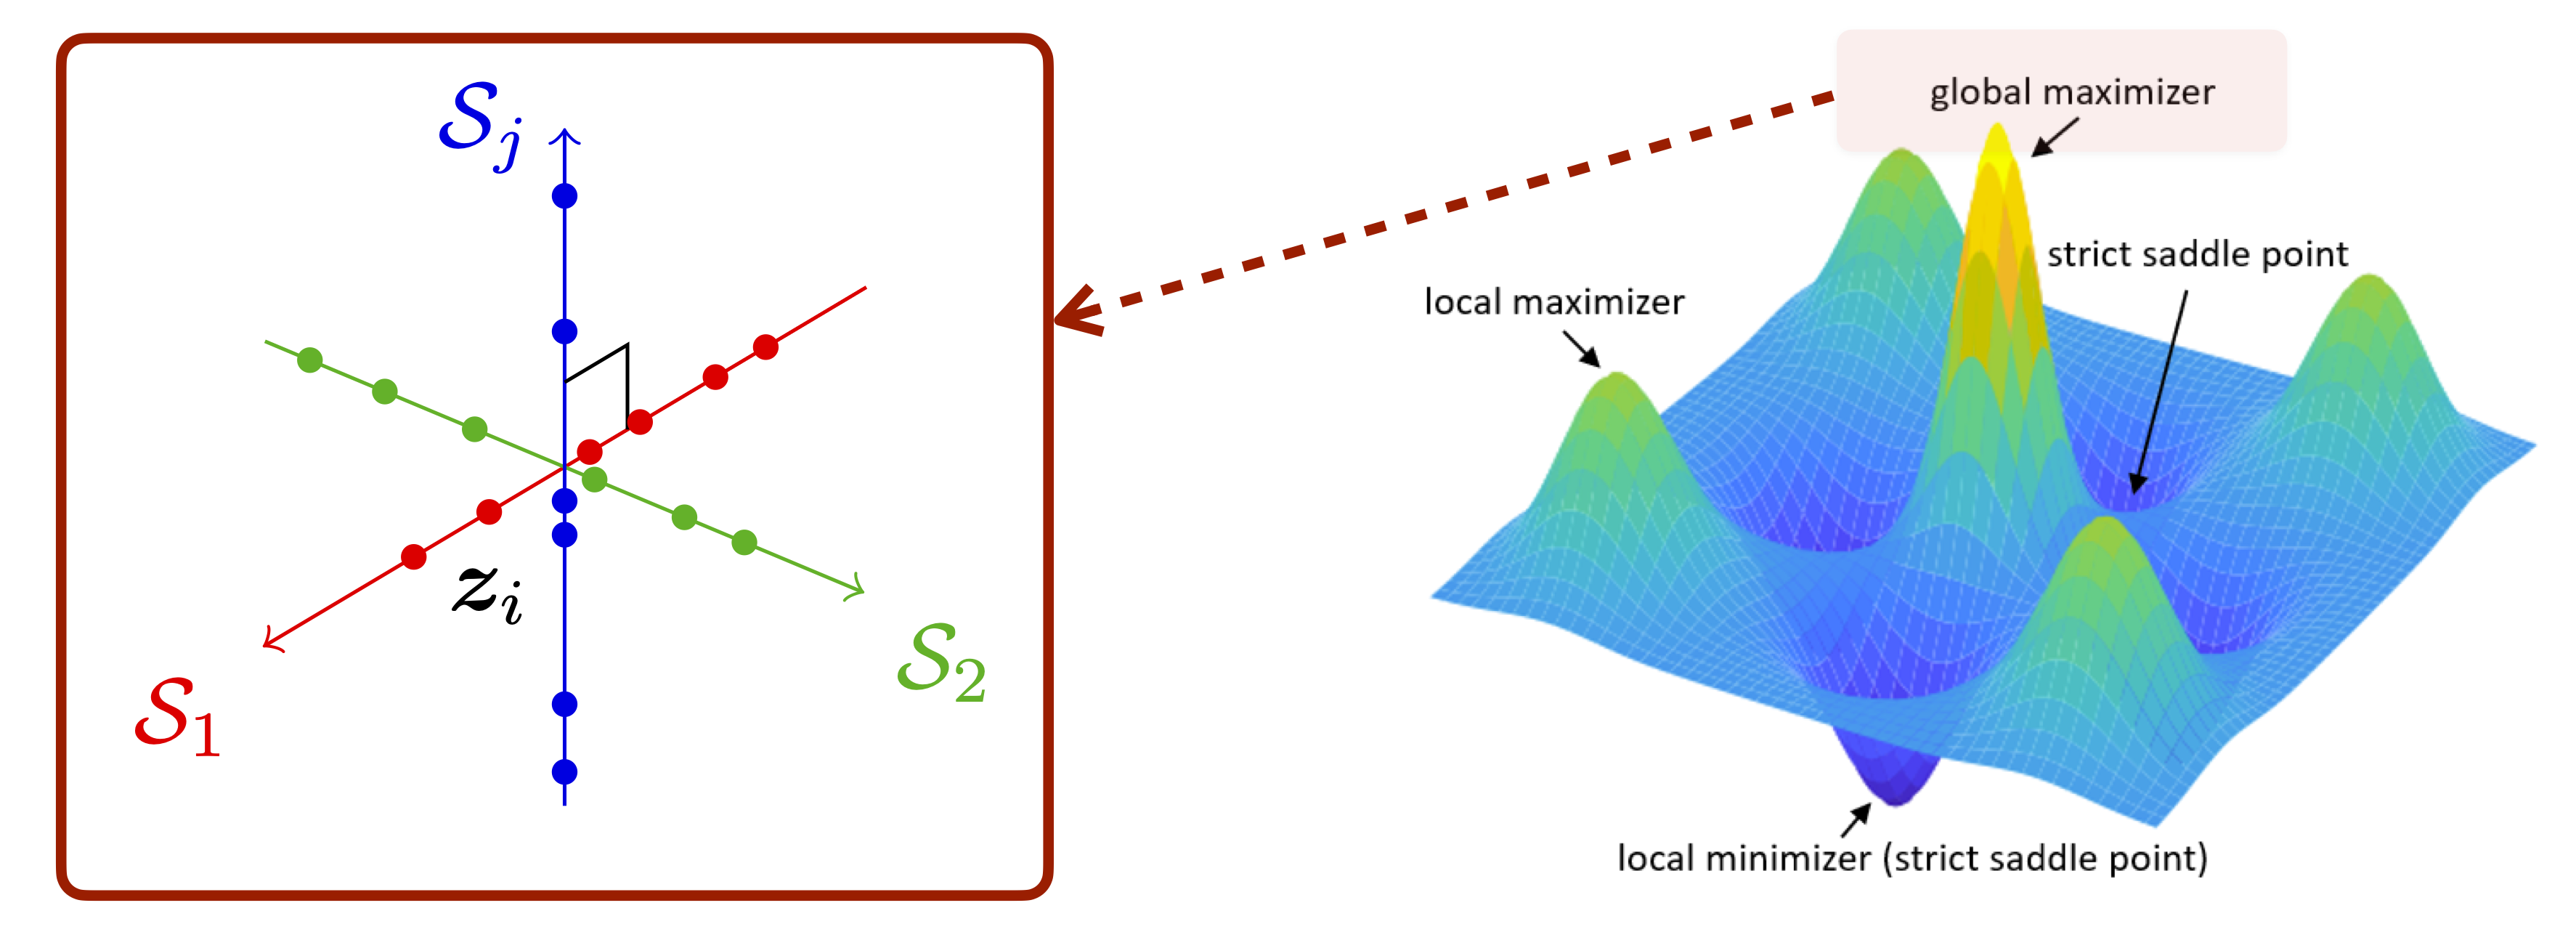
\includegraphics[width=0.8\linewidth]{\toplevelprefix/chapters/chapter3/figs/mcr2-global.png}
	\caption{{\bf Peisaj local de optimizare:} Conform Teoremei \ref{thm:MCR2-properties}, maximul global al obiectivului de reducere a ratei corespunde unei soluții cu subspații mutual incoerente.}
	\label{fig:mcr-global}
\end{figure}

\vspace{-0.1in}

\subsection{Proprietăți de Optimizare ale Reducerii Ratei de Codare}
\label{sec:MCR-landscape}

În această subsecțiune, studiem proprietățile de optimizare ale funcției MCR$^2$ prin analizarea soluțiilor sale optime și a structurii peisajului său de optimizare. Pentru a evita dificultatea tehnică introdusă de rețelele neuronale, considerăm o versiune simplificată a Problemei \eqref{eqn:maximal-rate-reduction} după cum urmează:
\begin{align}\label{eqn1:maximal-rate-reduction}
    \max_{\bm Z}\ R_{\epsilon}(\Z) - R_{\epsilon}^c(\Z)\qquad \mathrm{s.c.}\quad \|\bm Z_k\|_F^2 = N_k,\ k =1,\dots,K. 
\end{align}
În teorie, principiul MCR$^2$ \eqref{eqn1:maximal-rate-reduction} beneficiază de o mare generalizabilitate și poate fi aplicat reprezentărilor $\Z$ ale {\em oricăror} distribuții atâta timp cât ratele $R_\epsilon$ și $R^c_\epsilon$ pentru distribuții pot fi evaluate precis și eficient. Reprezentarea optimă $\Z^{\ast}$ ar trebui să aibă unele proprietăți geometrice și statistice interesante. Aici dezvăluim proprietăți frumoase ale reprezentării optime cu cazul special al subspațiilor, care au multe cazuri de utilizare importante în învățarea automată. Când reprezentarea dorită pentru $\Z$ este mai multe subspații, ratele $R_\epsilon$ și $R^c_\epsilon$ în \eqref{eqn1:maximal-rate-reduction} sunt date de \eqref{chap4-eqn:coding-length-eval} și \eqref{chap4-eqn:compress-loss-eval}, respectiv. La reducerea maximă a ratei, MCR$^2$ își atinge reprezentările optime, notate ca $\Z^{\ast} = [\Z_1^*,\dots,\Z_K^*]$ cu $\rank{(\Z_{k}^*)}\le d_k$. Se poate arăta că $\Z^{\ast}$ are următoarele proprietăți dorite (vezi \cite{yu2020learning} pentru o declarație formală și demonstrații detaliate).

\begin{theorem}[\bf Caracterizarea Soluțiilor Optime Globale]
	Presupunem că $\Z^{\ast} = [\Z_1^*,\dots,\Z_K^*]$ este o soluție optimă globală a Problemei~\eqref{eqn1:maximal-rate-reduction}. Următoarele afirmații sunt valabile:
	\begin{itemize}
		\item {\em Discriminativă între clase}: Atâta timp cât spațiul ambiental este adecvat de mare ($d \ge \sum_{k=1}^{K} d_k$), subspațiile sunt toate ortogonale între ele, {\em adică}, $(\Z_{k}^*)^{\top} \Z_{l}^* = \bm{0}$ pentru $k \not= l$.
		\item {\em Reprezentare maxim diversă}:
		      Atâta timp cât precizia de codare este adecvat de înaltă, adică $\epsilon ^4 < c\cdot \min_{k}\left\{ \frac{N_k}{N}\frac{d^2}{d_k^2}\right\}$, unde $c>0$ este o constantă. Fiecare subspațiu își atinge dimensiunea maximă, adică $\mathrm{rank}{(\Z_{k}^*)}= d_k$. În plus, cele mai mari $d_k-1$ valori singulare ale lui $\Z_{k}^*$ sunt egale.
		      \label{thm:MCR2-properties}
	\end{itemize}
\end{theorem}

Această teoremă indică faptul că principiul MCR$^2$ promovează încorporarea datelor în mai multe subspații independente (așa cum este ilustrat în \Cref{fig:mcr-global}), cu caracteristici distribuite {\em izotropic} în fiecare subspațiu (cu excepția posibil a unei dimensiuni). În mod notabil, această teoremă confirmă, de asemenea, că caracteristicile învățate prin principiul MCR$^2$ prezintă proprietățile discriminative cu dimensiuni reduse dorite discutate în \Cref{subsec:LDR}. În plus, dintre toate aceste reprezentări discriminative, preferă pe cea cu cele mai mari dimensiuni în spațiul ambiental. Aceasta este substanțial diferită de obiectivul gâtuirii informaționale~\eqref{chap4-eqn:information-bottleneck}.

\begin{example}[Clasificarea Imaginilor pe CIFAR-10]
	Aici prezentăm cum obiectivul MCR$^2$ ajută la învățarea unor reprezentări mai bune decât entropia încrucișată \eqref{chap4-eqn:cross-entropy} pentru clasificarea imaginilor. Aici adoptăm arhitectura populară de rețea neuronală, ResNet-18~\cite{he2016deep}, pentru a modela maparea de caracteristici $\z = f(\x,\theta)$. Optimizăm parametrii rețelei neuronale $\theta$ pentru a maximiza reducerea ratei de codare. Evaluăm performanța cu setul de date de clasificare a imaginilor CIFAR10~\cite{krizhevsky2009learning}.

	\begin{figure}[t]
		\begin{subfigure}[t]{0.42\textwidth}
			\centering
			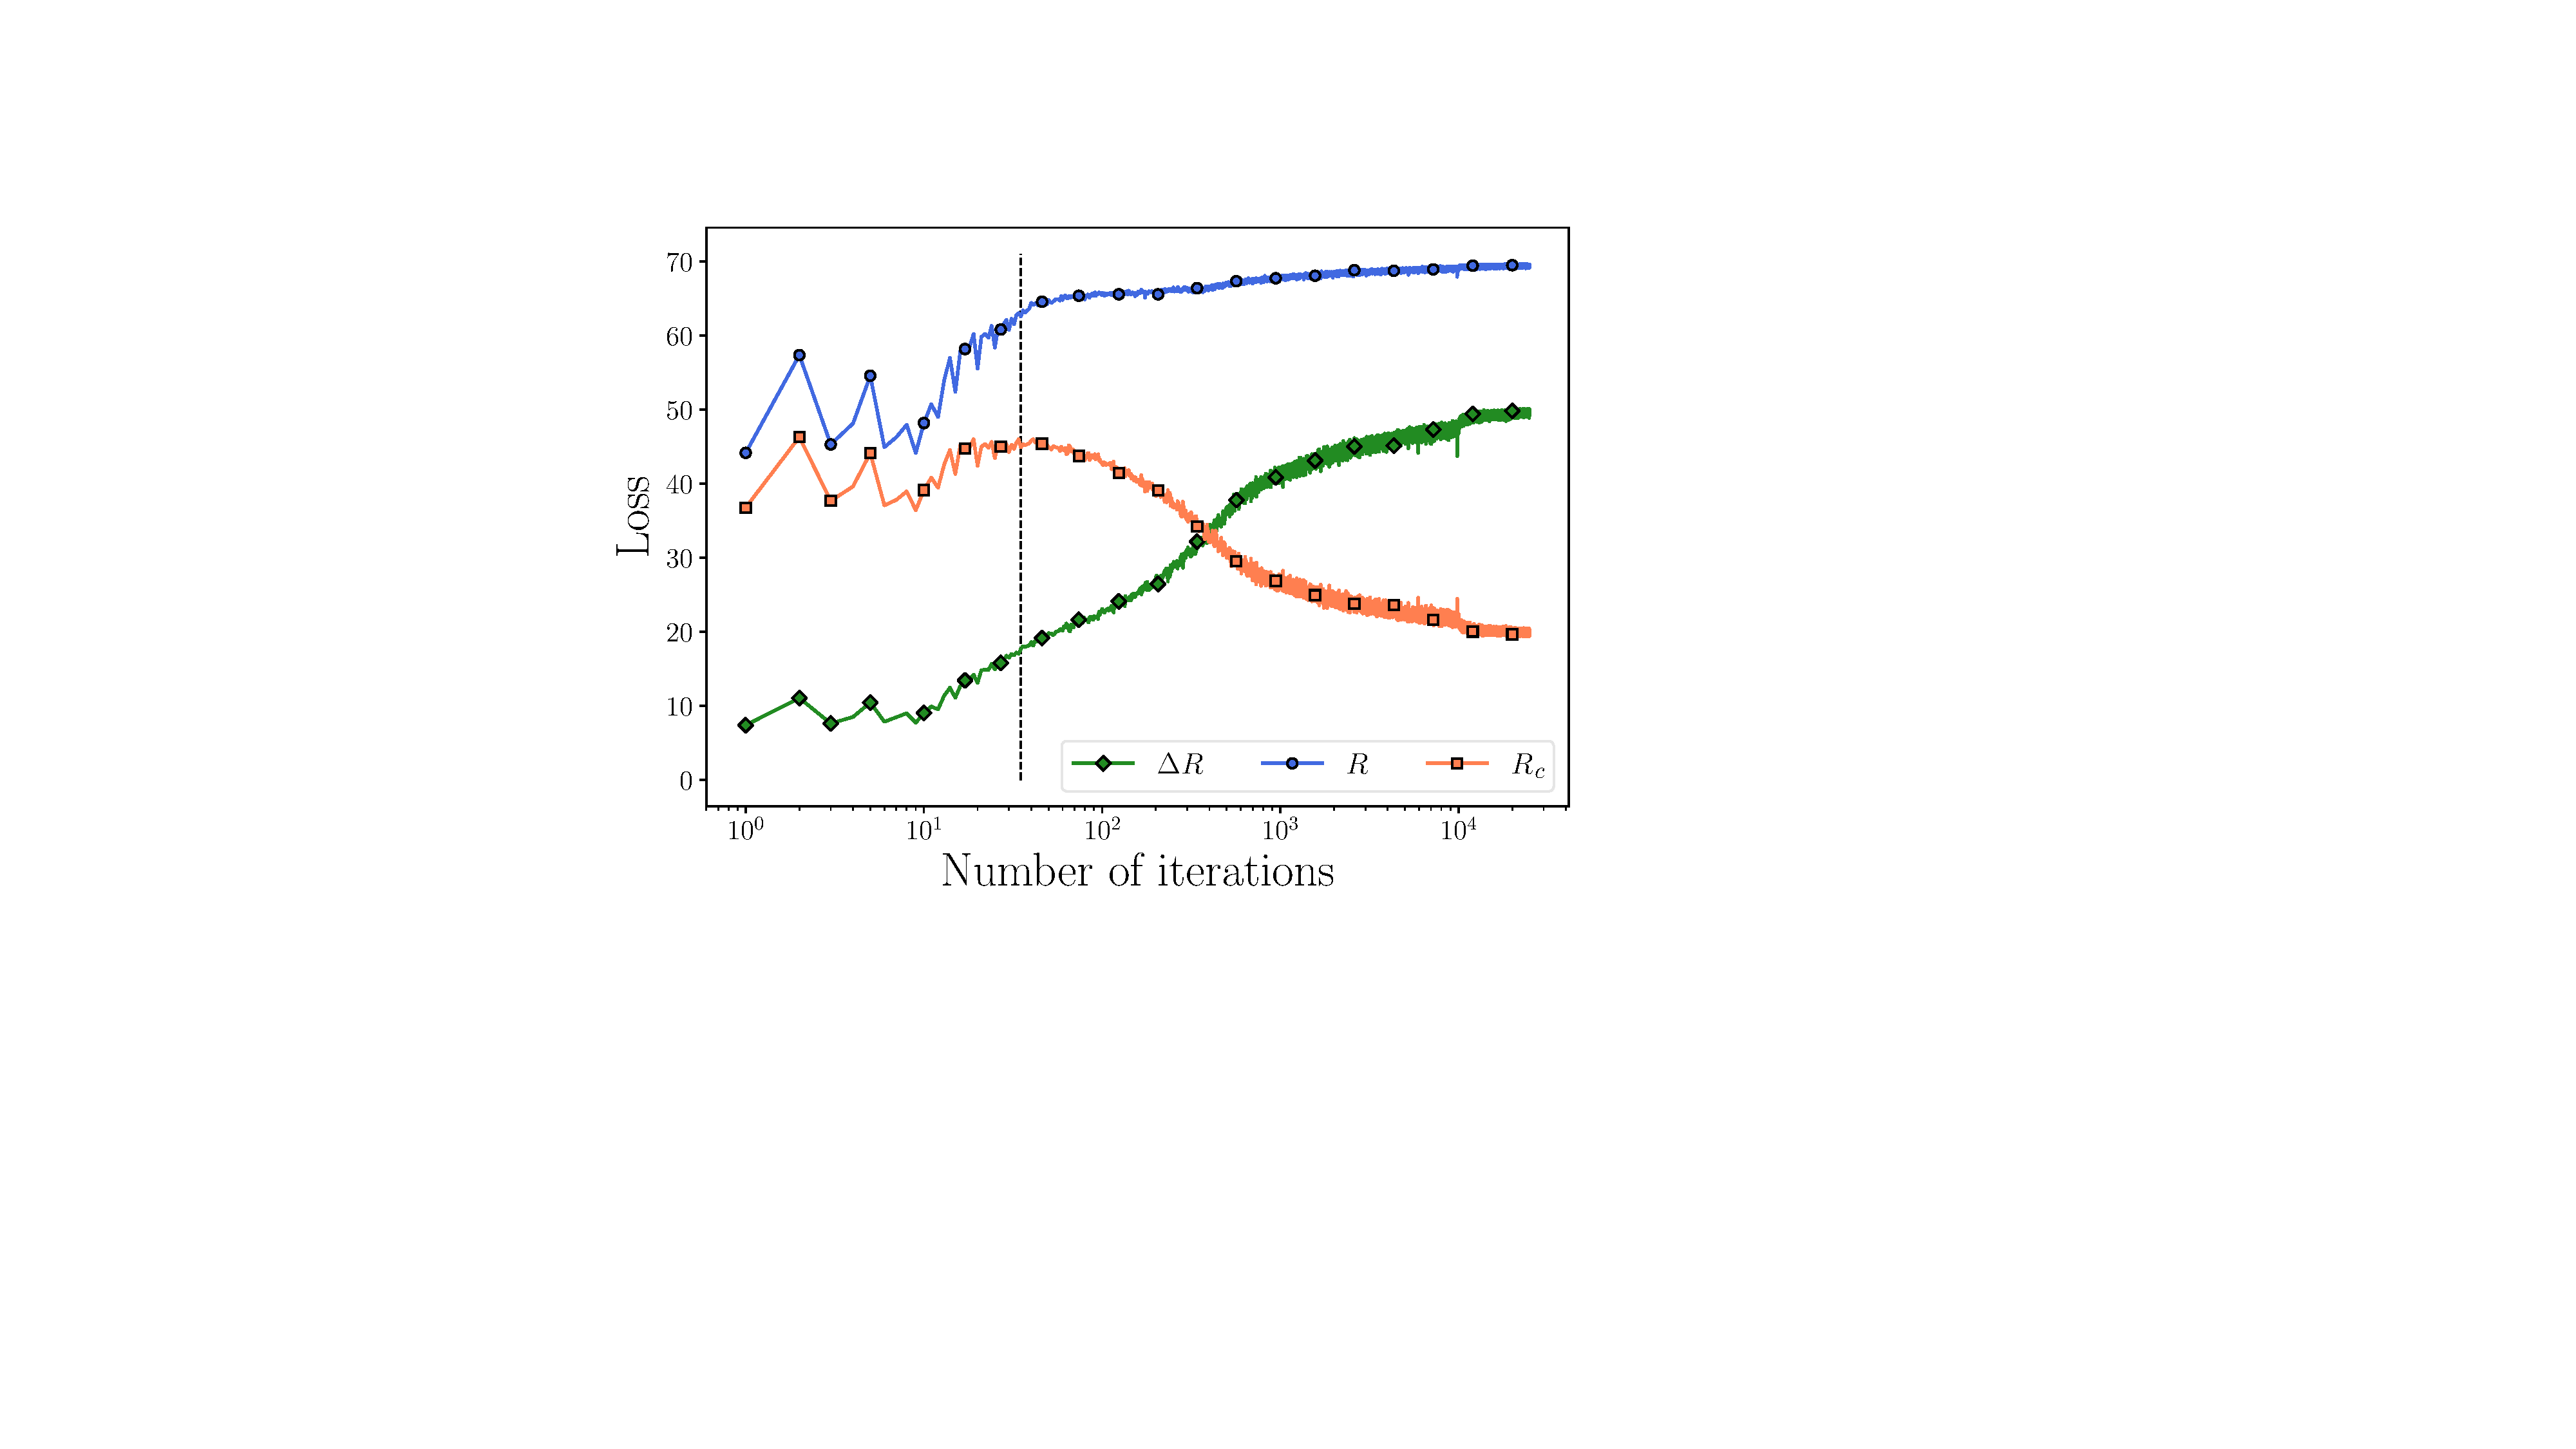
\includegraphics[width=\textwidth]{\toplevelprefix/chapters/chapter3/figs/loss_log.pdf}
			\caption{Evoluția lui $R_\epsilon$, $R^c_\epsilon$, $\Delta R_\epsilon$ în timpul procesului de antrenare.}
			\label{fig:train-test-loss-pca-1}
		\end{subfigure}
		\hfill
		\begin{subfigure}[t]{0.42\textwidth}
			\centering
			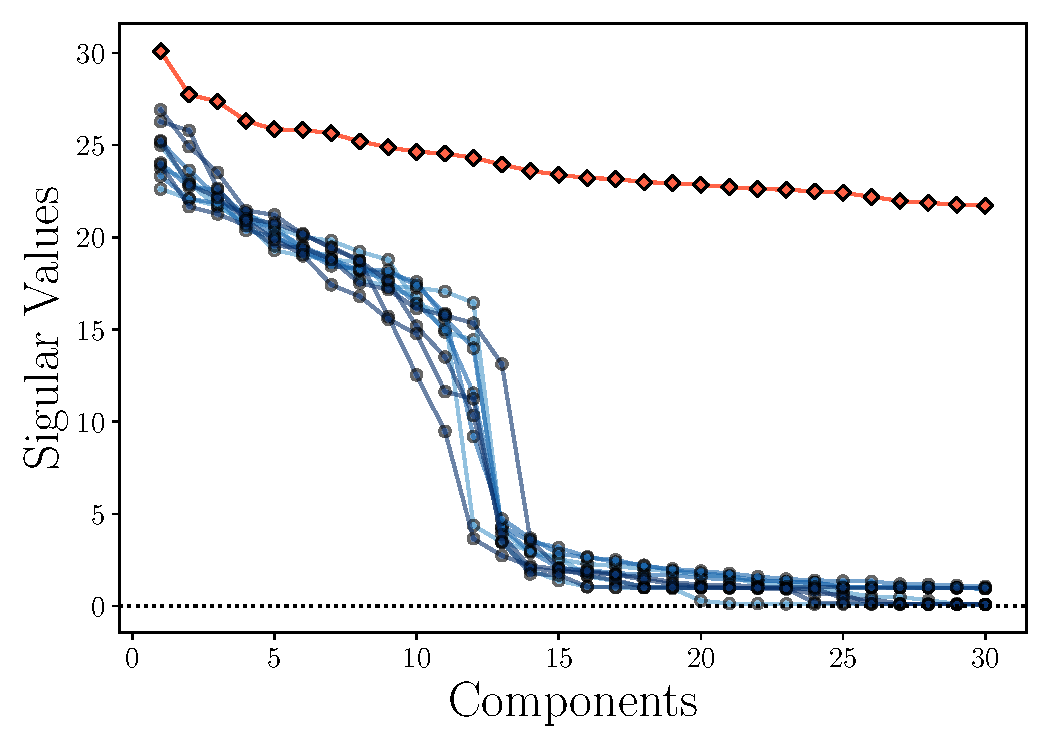
\includegraphics[width=\textwidth]{\toplevelprefix/chapters/chapter3/figs/pca_mainline.pdf}
			\caption{PCA: {\small (\textbf{roșu}) date generale; (\textbf{albastru}) clase individuale}.}
			\label{fig:train-test-loss-pca-3}
		\end{subfigure}
		\caption{\small Evoluția ratelor MCR$^2$ în procesul de antrenare, componentele principale ale caracteristicilor învățate.}
		\label{fig:train-test-loss-pca}
	\end{figure}

	\begin{figure*}[b]
		\begin{center}
			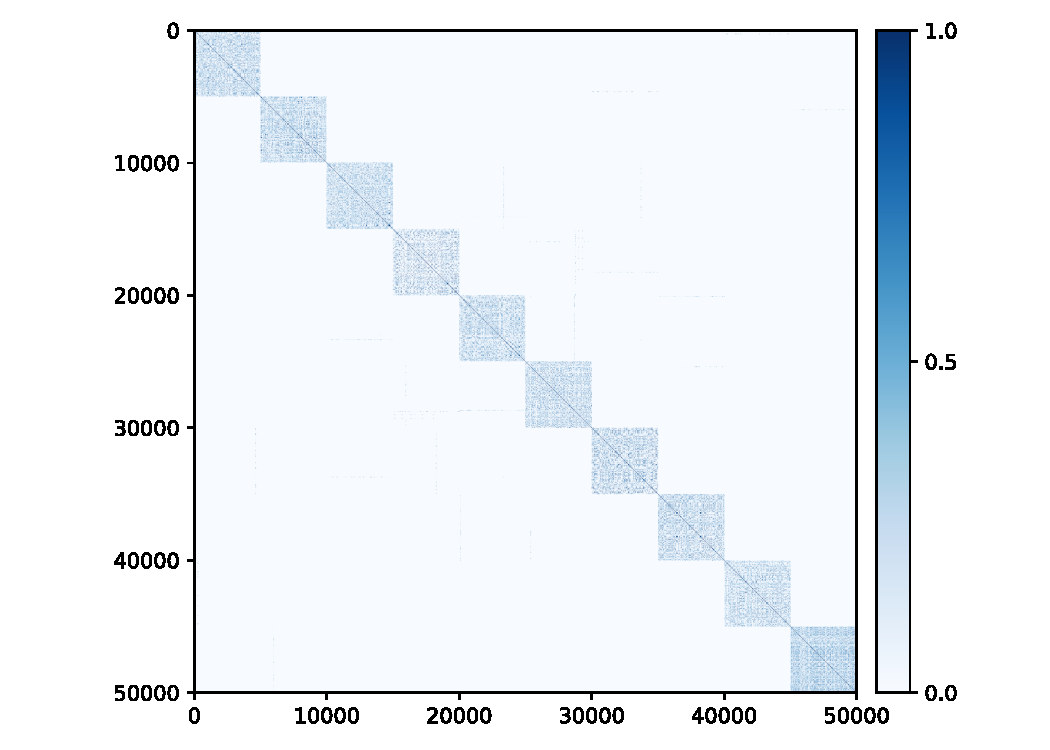
\includegraphics[width=0.42\textwidth]{\toplevelprefix/chapters/chapter3/figs/heatmap_mcr2.pdf}
			\hspace{0.25cm}
			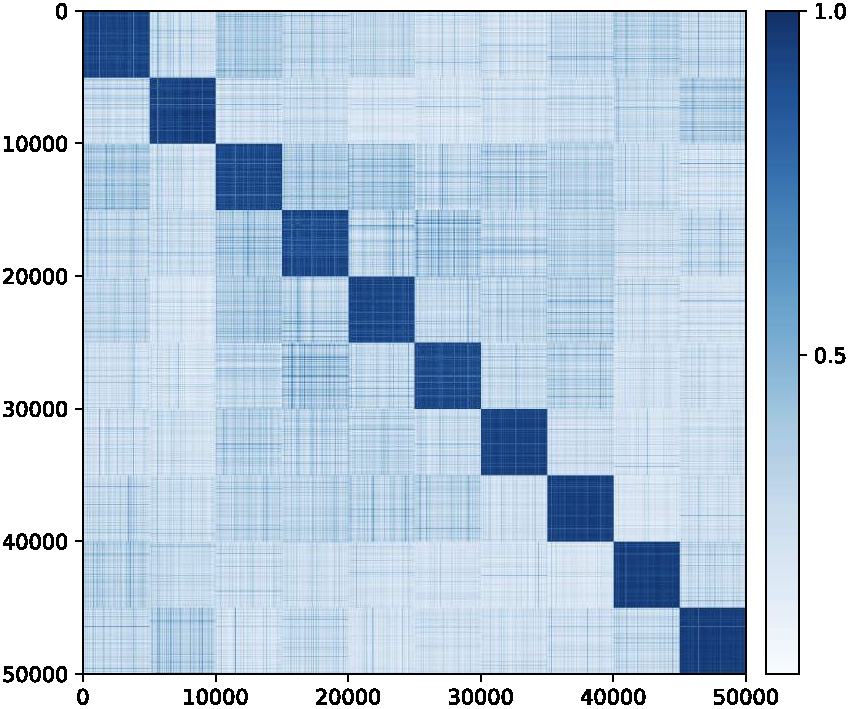
\includegraphics[width=0.42\textwidth]{\toplevelprefix/chapters/chapter3/figs/heatmap_ce.png}
			\caption{\small Similaritate cosinus între caracteristicile învățate folosind obiectivul MCR$^2$ (\textbf{stânga}) și pierderea CE (\textbf{dreapta}).}
			\label{fig:heatmap-plot}
		\end{center}
		\vskip -0.1in
	\end{figure*}

	\Cref{fig:train-test-loss-pca-1} ilustrează cum cele două rate și diferența lor (atât pentru datele de antrenare, cât și pentru cele de test) evoluează pe parcursul epocilor de antrenare: După o fază inițială, $R_\epsilon$ crește treptat în timp ce $R^c_\epsilon$ scade, indicând că caracteristicile $\bm Z$ se extind ca întreg în timp ce fiecare clasă $\bm Z_k$ este comprimată.
	\Cref{fig:train-test-loss-pca-3} arată distribuția valorilor singulare pe $\Z_k$. \Cref{fig:heatmap-plot} arată similaritățile cosinus între caracteristicile învățate sortate pe clasă. Comparăm similaritățile caracteristicilor învățate folosind entropia încrucișată \eqref{chap4-eqn:cross-entropy} și obiectivul MCR$^2$ \eqref{eqn:maximal-rate-reduction}. Din grafice, se poate vedea clar că reprezentările învățate folosind pierderea MCR$^2$ sunt mult mai diverse decât cele învățate folosind pierderea de entropie încrucișată. Mai multe detalii ale acestui experiment pot fi găsite în \cite{chan2021redunet}.
	\label{eg:Rate-Reduction-CIFAR10}
\end{example}

Cu toate acestea, a existat o lipsă aparentă de justificare a arhitecturilor de rețea folosite în experimentele de mai sus. Nu este încă clar de ce rețeaua adoptată aici (ResNet-18) este potrivită pentru reprezentarea hărții $f(\x, \theta)$, cu atât mai puțin pentru interpretarea operatorilor de strat și a parametrilor $\theta$ învățați în interior. În următorul capitol, {\em vom arăta cum să derivăm arhitecturile și componentele de rețea în întregime ca o „cutie albă" din obiectivul dorit (să zicem reducerea ratei)}.

\paragraph{MCR$^2$ regularizat.}
Teorema de mai sus caracterizează proprietățile optimelor globale ale obiectivelor de reducere a ratei. Dar ce se întâmplă cu alte optime, cum ar fi cele locale? Din cauza constrângerilor normei Frobenius, este o sarcină dificilă să analizăm Problema \eqref{eqn1:maximal-rate-reduction} dintr-o perspectivă teoretică de optimizare. Prin urmare, considerăm formularea Lagrangiană a \eqref{eqn1:maximal-rate-reduction}. Aceasta poate fi văzută ca o relaxare strânsă sau chiar o problemă echivalentă a \eqref{eqn1:maximal-rate-reduction} ale cărei soluții optime sunt de acord în setări specifice ale parametrului de regularizare; vezi \cite[Propozițiunea 1]{wang2024global}.
În mod specific, formularea pe care o studiem, denumită de acum înainte ca {\textit{problema MCR$^2$ regularizată}}, este următoarea:
\begin{align}\label{eq:MCR-reg}
	\max_{\bm Z}\ R_{\epsilon}(\Z) - R_{\epsilon}^c(\Z) - \frac{\lambda}{2}\|\bm Z\|_F^2,
\end{align}
unde $\lambda > 0$ este parametrul de regularizare. Deși programul \eqref{eq:MCR-reg} este extrem de neconcav și implică inverse de matrice în calculul gradientului său, putem totuși caracteriza explicit optimele sale locale și globale după cum urmează.

\begin{theorem}[\bf Optime Locale și Globale]\label{thm:mcr-global-opt}
	Fie $N_k$ numărul de eșantioane de antrenare din clasa $k$ pentru fiecare $k \in \{1,\dots,K\}$, $N_{\max} \doteq \max\{N_1,\dots,N_K\}$, $\alpha=d/(N\epsilon^2)$, și $\alpha_{k} = d/(N_k\epsilon^2)$ pentru fiecare $k \in \{1,\dots,K\}$. Dată fiind o precizie de codare $\epsilon > 0$, dacă parametrul de regularizare satisface
	\begin{align}\label{eq:lambda}
		\lambda \in \left(0, \frac{d(\sqrt{N/N_{\max}}-1)}{N(\sqrt{N/N_{\max}}+1)\epsilon^2} \right],
	\end{align}
	atunci următoarele afirmații sunt valabile: \\
	(i) ({\bf Maximizatori locali}) $\bm Z^* = \left[\bm Z_1^*,\dots,\bm Z_K^* \right]$ este un maximizator local al Problemei \eqref{eq:MCR-reg} dacă și numai dacă blocul $k$ admite următoarea descompunere
	\begin{align}\label{eq:Zk opti}
		\bm Z_k^* = \left(\frac{ \eta_k + \sqrt{\eta_k^2 - 4\lambda^2N/N_k}}{2\lambda \alpha_{k}}\right)^{1/2} \bm U_k \bm V_k^\top,
	\end{align}
	unde (a) $r_k = \mathrm{rank}(\bm Z_k^*)$ satisface $r_k \in [0,\min\{N_k,d\})$ și $\sum_{k=1}^K r_k \le \min\{N,d\}$, (b) $\bm U_k \in \mathcal{O}^{d \times r_k}$ satisface $\bm U_k^{\top}\bm U_l = \bm 0$ pentru toți $k \neq l$, $\bm V_k \in \mathcal{O}^{N_k \times r_k}$, și (c) $\eta_k=(\alpha_k-\alpha) - \lambda(N/N_k+1)$ pentru fiecare $k\in \{1,\dots,K\}$.
	\\
	(ii) ({\bf Maximizatori globali}) $\bm Z^* = \left[\bm Z_1^*,\dots,\bm Z_K^* \right]$ este un maximizator global al Problemei \eqref{eq:MCR-reg} dacă și numai dacă (a) satisface toate condițiile de mai sus și $\sum_{k=1}^K r_k = \min\{m,d\}$, și (b) pentru toți $k \neq l \in [K]$ satisfăcând $N_k < N_l$ și $r_l > 0$, avem $r_k = \min\{N_k,d\}$.
\end{theorem}

\begin{figure}[t]
	\centering
	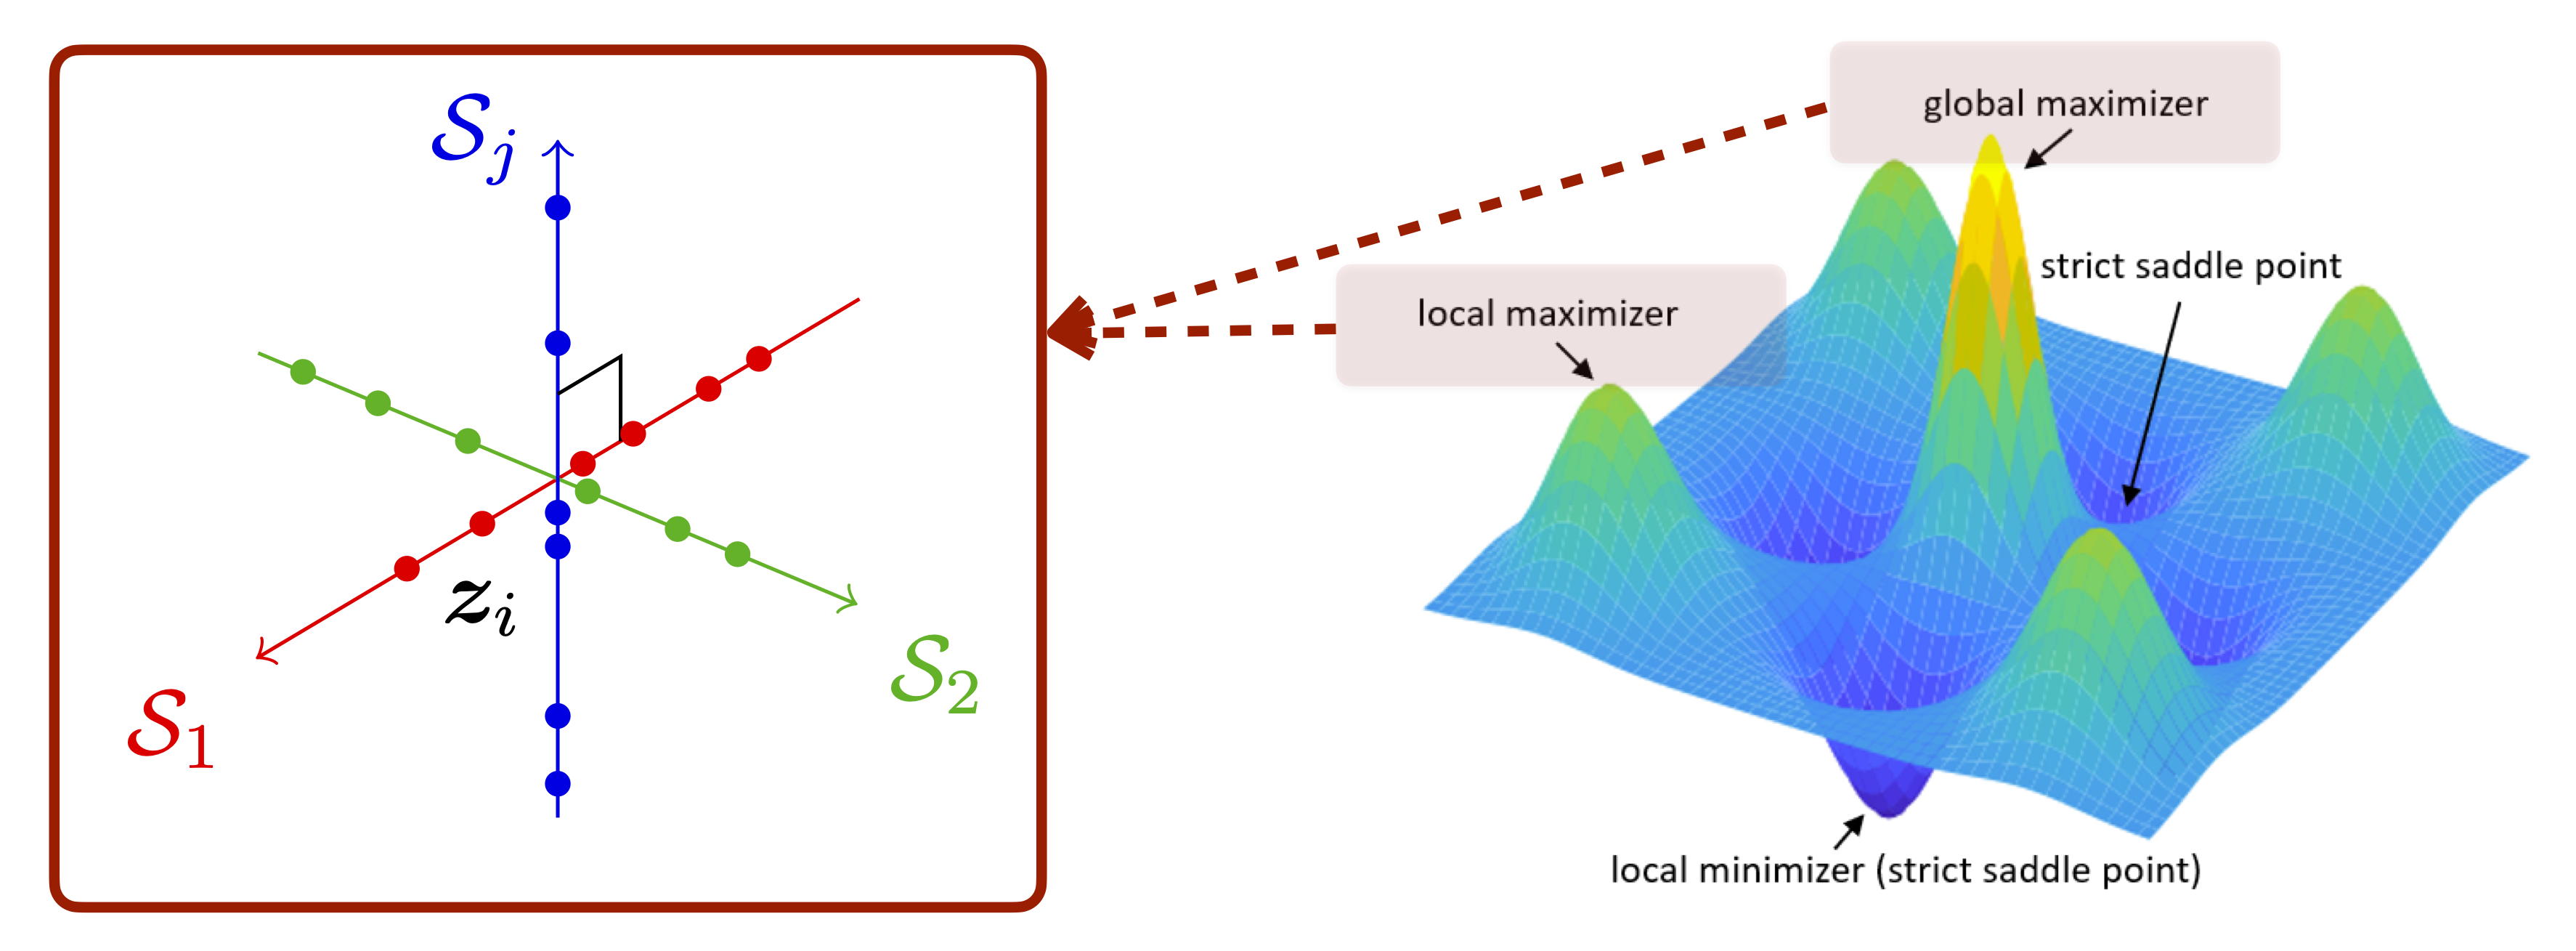
\includegraphics[width=0.8\linewidth]{\toplevelprefix/chapters/chapter3/figs/mcr2-global-local.png}
	\caption{{\bf Peisaj global de optimizare:} Conform \cite{sun2015nonconvex,lee2016gradient}, \Cref{thm:mcr-global-opt,thm:mcr-benign-opt-landscape}, atât maximele globale, cât și cele locale ale obiectivului (regularizat) de reducere a ratei corespund unei soluții cu subspații mutual incoerente. Toate celelalte puncte critice sunt puncte de șa stricte.}
	\label{fig:mcr-global-local}
\end{figure}

Această teoremă caracterizează explicit optimele locale și globale ale problemei \eqref{eq:MCR-reg}. Intuitiv, aceasta arată că caracteristicile reprezentate de fiecare maximizator local al Problemei \eqref{eq:MCR-reg} sunt cu dimensiuni reduse și discriminative. Deși am caracterizat soluțiile optime locale și globale în Teorema~\ref{thm:mcr-global-opt}, rămâne necunoscut dacă aceste soluții pot fi calculate eficient folosind GD pentru a rezolva problema \eqref{eq:MCR-reg}, deoarece GD se poate bloca la alte puncte critice, cum ar fi un punct de șa.
Din fericire, \cite{sun2015nonconvex,lee2016gradient} au arătat că dacă o funcție este de două ori continuu diferențiabilă și satisface {\em proprietatea de șa strictă}, adică fiecare punct critic este fie un minimizator local, fie un punct de șa strict\footnote{Spunem că un punct critic este un punct de șa strict al Problemei \eqref{eq:MCR-reg} dacă are o direcție cu curbură strict pozitivă~\cite{sun2015nonconvex}. Aceasta include puncte de șa clasice cu curbură strict pozitivă, precum și minimizatori locali.}, GD converge la minimizatorul său local aproape sigur cu inițializare aleatorie. Investigăm peisajul global de optimizare al problemei \eqref{eq:MCR-reg} prin caracterizarea tuturor punctelor sale critice după cum urmează.

\begin{theorem}[\bf Peisaj Global de Optimizare Benign]\label{thm:mcr-benign-opt-landscape}
	Dată fiind o precizie de codare $\epsilon > 0$, dacă parametrul de regularizare satisface \eqref{eq:lambda}, se susține că orice punct critic $\bm Z$ al problemei \eqref{eq:MCR-reg} este fie un maximizator local, fie un punct de șa strict.
\end{theorem}
Împreună, cele două teoreme de mai sus arată că caracteristicile învățate asociate cu fiecare maximizator local al obiectivului de reducere a ratei---nu doar maximizatorii globali---sunt structurate ca subspații incoerente cu dimensiuni reduse. Mai mult, obiectivul (regularizat) de reducere a ratei \eqref{eqn:maximal-rate-reduction} are un peisaj foarte benign cu doar maxime locale și șei stricte ca puncte critice, așa cum este ilustrat în \Cref{fig:mcr-global-local}.
Conform \cite{sun2015nonconvex,lee2016gradient}, \Cref{thm:mcr-global-opt,thm:mcr-benign-opt-landscape} implică faptul că reprezentările cu dimensiuni reduse și discriminative (LDR) pot fi găsite eficient prin aplicarea coborârii gradientului (stochastic) la obiectivul de reducere a ratei \eqref{eqn:maximal-rate-reduction} din inițializare aleatorie. Aceste rezultate explică, de asemenea, indirect de ce în \Cref{eg:Rate-Reduction-CIFAR10}, dacă rețeaua aleasă este suficient de expresivă și antrenată bine, reprezentarea rezultată oferă de obicei o reprezentare liniară incoerentă care corespunde probabil soluției optime globale.
Cititorii interesați sunt referiți la \cite{wang2024global} pentru demonstrații.

\section{Rezumat și Note}

Utilizarea denoising-ului și difuziei pentru eșantionare are o istorie bogată. Prima lucrare care este clar despre un model de difuzie este probabil \cite{Sohl-Dickstein2015}, dar înainte de aceasta există multe lucrări despre denoising ca problemă computațională și statistică. Cea mai relevantă dintre acestea este probabil \cite{hyvarinen05a}, care folosește explicit funcția de scor pentru denoising (precum și pentru a efectua analiza componentelor independente). Cele mai populare urmări sunt practic co-apărute: \cite{ho2020denoising,song2019}. De atunci, mii de lucrări s-au bazat pe modele de difuzie; vom revizita acest subiect în \Cref{ch:autoencoding}.

Multe dintre aceste lucrări folosesc un proces stochastic diferit de combinația liniară simplă \eqref{eq:gen_additive_gaussian_noise_model}. De fapt, toate lucrările enumerate mai sus subliniază necesitatea de a adăuga zgomot gaussian \textit{independent} la începutul fiecărui pas al procesului înainte. Lucrarea orientată teoretic folosește de fapt mișcarea browniană sau ecuații diferențiale stochastice pentru a formula procesul înainte \cite{song2020score}. Cu toate acestea, deoarece combinațiile liniare de gaussiene rezultă tot în gaussiene, \textit{distribuțiile marginale} ale acestor procese iau încă forma \eqref{eq:gen_additive_gaussian_noise_model}. Cea mai mare parte a discuției noastre necesită doar ca distribuțiile marginale să fie ceea ce sunt, și prin urmare modelul nostru excesiv de simplist este de fapt destul pentru aproape totul. De fapt, singura dată când distribuțiile marginale nu sunt suficiente este când derivăm o expresie pentru \(\Ex[\vx_{s} \mid \vx_{t}]\) în termenii lui \(\Ex[\vx \mid \vx_{t}]\). Diferite procese (de zgomot) dau diferite astfel de expresii, care pot fi folosite pentru eșantionare (și desigur există și alte moduri de a deriva eșantionatoare eficiente, cum ar fi mereu popularul eșantionator DDPM). Procesul din \eqref{eq:gen_additive_gaussian_noise_model} este, totuși, un proces stochastic de bună credință, a cărui iterație de denoising „naturală" ia forma popularului algoritm DDIM \cite{song2020denoising}. (Chiar și această echivalență nu este trivială; cităm \cite{de2025distributional} ca justificare.)

Pe lângă lucrarea teoretică \citep{li2024d} acoperită în \Cref{sec:denoising-intro}, și linia de lucrări pe care o construiește, care studiază eficiența de \textit{eșantionare} a modelelor de difuzie când datele au structură cu dimensiuni reduse, există un corp mare de lucrări care studiază eficiența de \textit{antrenare} a modelelor de difuzie când datele au structură cu dimensiuni reduse. În mod specific, \citet{chen2023score} și \citep{wang2024diffusion} au caracterizat eroarea de aproximare și estimare a denoiserilor când datele aparțin unui amestec de gaussiene de rang redus, arătând că numărul de eșantioane de antrenare necesare pentru a învăța cu precizie distribuția scalează cu dimensiunea intrinsecă a datelor mai degrabă decât cu distribuția ambientală. Există o lucrare \textit{metodologică} considerabilă care încearcă să utilizeze structura cu dimensiuni reduse a datelor pentru a face diverse lucruri cu modele de difuzie. Evidențiem trei aici: editarea imaginii \citep{chen2024exploring}, filigranul \citep{li2024shallow} și dezînvățarea \citep{chen2025dual}, deși, ca întotdeauna, aceasta este o listă neexhaustivă.

\section{Exerciții și Extensii}

\begin{exercise}
    Vă rugăm să arătați că \eqref{eq:optimal_denoiser} este soluția optimă a Problemei \eqref{eq:denoising_loss}.
\end{exercise}

\begin{exercise}\label{exercise:conditional_gaussian}
  Considerați vectorii aleatori $\vx \in \bR^D$ și $\vy \in \bR^d$, astfel încât perechea $(\vx, \vy) \in \bR^{D + d}$ este în comun gaussiană. Aceasta înseamnă că
  \begin{equation*}
    \begin{bmatrix}
      \vx \\
      \vy
    \end{bmatrix}
    \sim
    \cN \left(
      \begin{bmatrix}
        \vmu_{\vx} \\
        \vmu_{\vy}
      \end{bmatrix}
      ,
      \begin{bmatrix}
        \vSigma_{\vx} & \vSigma_{\vx\vy} \\
        \vSigma_{\vx\vy}^\top & \vSigma_{\vy}
      \end{bmatrix}
    \right),
  \end{equation*}
  unde parametrii de medie și covarianță sunt dați de
  \begin{equation*}
    \vmu_{\vx} = \bE[\vx],\quad \vmu_{\vy} = \bE[\vy],\quad
    \begin{bmatrix}
      \vSigma_{\vx} & \vSigma_{\vx\vy} \\
      \vSigma_{\vx\vy}^\top & \vSigma_{\vy}
    \end{bmatrix}
    =
    \bE\left[
      \begin{bmatrix}
        \vx - \bE[\vx] \\
        \vy - \bE[\vy]
      \end{bmatrix}
      \begin{bmatrix}
        \vx - \bE[\vx] \\
        \vy - \bE[\vy]
      \end{bmatrix}^\top
      \right]
  \end{equation*}
  Presupunem că $\vSigma_{\vy}$ este pozitiv definită (prin urmare inversabilă); atunci semipozitivitatea matricei de covarianță este echivalentă cu condiția complementului Schur $\vSigma_{\vx} - \vSigma_{\vx\vy} \vSigma_{\vy}^{-1} \vSigma_{\vx\vy}^\top \succeq \Zero$.

  În acest exercițiu, vom demonstra că distribuția condiționată $p_{\vx \mid \vy}$ este gaussiană: și anume,
  \begin{equation}\label{eq:gaussian-conditional-eqn}
    p_{\vx \mid \vy} \sim \cN\left(
      \vmu_{\vx} + \vSigma_{\vx\vy} \vSigma_{\vy}^{-1} (\vy - \vmu_{\vy}),
      \vSigma_{\vx} - \vSigma_{\vx\vy} \vSigma_{\vy}^{-1}
      \vSigma_{\vx\vy}^{\top}
    \right).
  \end{equation}
  O cale directă pentru a demonstra acest rezultat manipulează raportul definitor al densităților $p_{\vx, \vy} / p_{\vy}$. Schițăm un argument algebric concis de această formă mai jos.

  \begin{enumerate}
    \item Verificați următoarea identitate matriceală pentru covarianță:
      \begin{equation}\label{eq:gaussian-conditional-covariance-block}
        \begin{bmatrix}
          \vSigma_{\vx} & \vSigma_{\vx\vy} \\
          \vSigma_{\vx\vy}^\top & \vSigma_{\vy}
        \end{bmatrix}
        =
        \begin{bmatrix}
          \vI_D & \vSigma_{\vx\vy}\vSigma_{\vy}^{-1} \\
          \Zero & \vI_d
        \end{bmatrix}
        \begin{bmatrix}
          \vSigma_{\vx} - \vSigma_{\vx\vy} \vSigma_{\vy}^{-1}
          \vSigma_{\vx\vy}^{\top} & \Zero \\
          \Zero & \vSigma_{\vy}
        \end{bmatrix}
        \begin{bmatrix}
          \vI_D & \Zero\\
          \vSigma_{\vy}^{-1}\vSigma_{\vx\vy}^\top & \vI_d
        \end{bmatrix}.
      \end{equation}
      Se ajunge la această identitate efectuând două runde de eliminare gaussiană (pe blocuri) pe matricea de covarianță.
    \item Pe baza identității anterioare, arătați că
      \begin{equation}\label{eq:gaussian-conditional-covariance-inverse-block}
        \begin{bmatrix}
          \vSigma_{\vx} & \vSigma_{\vx\vy} \\
          \vSigma_{\vx\vy}^\top & \vSigma_{\vy}
        \end{bmatrix}^{-1}
        =
        \begin{bmatrix}
          \vI_D & \Zero\\
          -\vSigma_{\vy}^{-1}\vSigma_{\vx\vy}^\top & \vI_d
        \end{bmatrix}
        \begin{bmatrix}
          \left(\vSigma_{\vx} - \vSigma_{\vx\vy} \vSigma_{\vy}^{-1}
          \vSigma_{\vx\vy}^{\top}\right)^{-1} & \Zero \\
          \Zero & \vSigma_{\vy}^{-1}
        \end{bmatrix}
        \begin{bmatrix}
          \vI_D & -\vSigma_{\vx\vy}\vSigma_{\vy}^{-1} \\
          \Zero & \vI_d
        \end{bmatrix}
      \end{equation}
      ori de câte ori inversele relevante sunt definite.\footnote{În cazurile în care termenul complement Schur nu este inversabil, același rezultat este valabil cu inversa sa înlocuită de pseudoinversa Moore-Penrose. În special, distribuția condiționată \eqref{eq:gaussian-conditional-eqn} devine o distribuție gaussiană degenerată.}
      Concluzionați că
      \begin{align}
        &\begin{bmatrix}
          \vx-\vmu_{\vx} \\
          \vy-\vmu_{\vy}
        \end{bmatrix}^{\top}
        \begin{bmatrix}
          \vSigma_{\vx} & \vSigma_{\vx\vy} \\
          \vSigma_{\vx\vy}^\top & \vSigma_{\vy}
        \end{bmatrix}^{-1}
        \begin{bmatrix}
          \vx-\vmu_{\vx} \\
          \vy-\vmu_{\vy}
        \end{bmatrix}
        \\
        &\qquad=
        \begin{bmatrix}
          \vx - \left(\vmu_{\vx} + \vSigma_{\vx\vy}\vSigma_{\vy}^{-1}(\vy
          - \vmu_{\vy})\right) \\
          \vy - \vmu_{\vy}
        \end{bmatrix}^\top
        \begin{bmatrix}
          \left(\vSigma_{\vx} - \vSigma_{\vx\vy} \vSigma_{\vy}^{-1}
          \vSigma_{\vx\vy}^{\top}\right)^{-1} & \Zero \\
          \Zero & \vSigma_{\vy}^{-1}
        \end{bmatrix}
        \begin{bmatrix}
          \vx - \left(\vmu_{\vx} + \vSigma_{\vx\vy}\vSigma_{\vy}^{-1}(\vy
          - \vmu_{\vy})\right) \\
          \vy - \vmu_{\vy}
        \end{bmatrix}.
      \end{align}
      (\textit{Indicație: Pentru a economisi manipulări algebrice, rețineți că prima și ultima matrice din partea dreaptă a \Cref{eq:gaussian-conditional-covariance-block} sunt transpuse una a celeilalte.})
    \item Împărțind $p_{\vx, \vy} / p_{\vy}$, demonstrați \Cref{eq:gaussian-conditional-eqn}. (\textit{Indicație: Folosind identitățile anterioare, ar trebui să fie necesară doar algebră minimă. Pentru constanta de normalizare, folosiți \Cref{eq:gaussian-conditional-covariance-inverse-block} pentru a factoriza determinantul în mod similar.})
  \end{enumerate}
\end{exercise}

\begin{exercise}\label{exercise:sherman_morrison_woodbury_identity}
    Arătați identitatea Sherman-Morrison-Woodbury, adică pentru matricele \(\vA\), \(\vC\), \(\vU\), \(\vV\) astfel încât \(\vA\), \(\vC\) și \(\vA + \vU\vC\vV\) sunt inversabile,
    \begin{equation}
        (\vA + \vU\vC\vV)^{-1} = \vA^{-1} - \vA^{-1}\vU(\vC^{-1} + \vV\vA^{-1}\vU)^{-1}\vV\vA^{-1}
    \end{equation}
\end{exercise}

\begin{exercise}\label{exercise:generalizing_results_to_different_noise_models}
    Rederivați următoarele, presupunând că \(\vx_{t}\) urmează modelul de zgomot generalizat \eqref{eq:gen_additive_gaussian_noise_model}.
    \begin{itemize}
        \item Formula lui Tweedie: \eqref{eq:gen_tweedie}.
        \item Iterația DDIM: \eqref{eq:gen_denoising_iteration}.
        \item Denoiserul optim Bayes pentru un model de amestec gaussian: \eqref{eq:gen_gmm_bayes_optimal_denoiser}.
    \end{itemize}
\end{exercise}

\begin{exercise}\label{exercise:implement_denoising_processes}
\begin{enumerate}
    \item Implementați formulele derivate în \Cref{exercise:generalizing_results_to_different_noise_models}, construind un eșantionator pentru amestecuri gaussiene.
    \item Reproduceți \Cref{fig:ve_forward_denoising} și \Cref{fig:vp_gmm_denoising}.
    \item Introducem acum un proces separat numit \textit{Potrivirea Fluxului (FM)}, după cum urmează:
    \begin{equation}
        \alpha_{t} = 1 - t, \qquad \sigma_{t} = t.
    \end{equation}
    Implementați acest proces folosind același cadru și testați-l pentru eșantionare în dimensiuni înalte. Care proces pare să dea rezultate mai bune sau mai stabile?
\end{enumerate}
\end{exercise}

\begin{exercise}
	Vă rugăm să arătați următoarele proprietăți ale funcției $\log\det(\cdot)$.
	\begin{enumerate}
		\item Arătați că
		      \begin{align*}
			      f(\vX) = \log\det\left(\vX\right)
		      \end{align*}
		      este o funcție concavă. ({\bf Indicație:} Funcția $f(\vx)$ este convexă dacă și numai dacă funcția $f(\vx+t\vh)$ pentru toți $\vx$ și $\vh$.)

		\item Arătați că:
		      \begin{align*}
			      \log\det(\vI + \vX^\top\vX) = \log\det(\vI + \vX\vX^\top)
		      \end{align*}

		\item Fie $\vA \in \R^{n\times n}$ o matrice pozitiv definită. Vă rugăm să arătați că:
		      \begin{align}
			      \log\det\left(\vA \right) = \sum_{i=1}^n \log(\lambda_i),
		      \end{align}
		      unde $\lambda_1,\lambda_2,\dots,\lambda_n$ sunt valorile proprii ale lui $\vA$.
	\end{enumerate}
\end{exercise}

\end{document}